%\documentclass[spanish]{beamer}
\documentclass[handout]{beamer} %ignorar overlays para imprimir
\usepackage{pgfpages}
%

% esto me setea la variable pdf dependiendo del valor de \pdfoutput, que es >0
% sólo cuando estoy usando pdflatex para compilar el documento
\newif\ifpdf
\ifnum\pdfoutput<0
\pdffalse\fi
\ifnum\pdfoutput=0
\pdffalse\fi
\ifnum\pdfoutput>0
\pdftrue\fi

%\makeatletter
%\def\markboth#1#2{\def\leftmark{\@IEEEcompsoconly{\sffamily}\MakeUppercase{\protect#1}}%
%\def\rightmark{\@IEEEcompsoconly{\sffamily}\MakeUppercase{\protect#2}}}
%\makeatother

%
% ===
% === I18n / L10n
% ===
%
% babel me da separación de sílabas para palabras en el idioma que le paso como
%       argumento opcional. <-- Éste hay que pasarlo en \documentclass
\usepackage[spanish]{babel}
%
% inputenc define la codificación de caracteres del código fuente, acá utf8.
\usepackage[utf8]{inputenc}
%
% ===
% === Gráficos
% ===
% 
% pst-pdf me permite usar PSTricks con pdflatex. Necesito cargarlo sólo si está
%         definida la variable pdf, por eso está entre \ifpdf ... \fi
%\ifpdf\usepackage{pst-pdf}\fi
%
% color me permite usar colores en el documento.
\usepackage{color}
%
% graphicx me da el comando \includegraphics para insertar imágenes (?)
\usepackage{graphicx}
%
% pstricks es un conjunto de macros basadas en PostScript para TeX, en
%          castellano, me da un entorno pstricks y comandos que uso dentro de
%          éste, que me sirven para dibujar figuras/diagramas/etc de manera
%          relativamente simple.
%\usepackage{pstricks}
%
% pst-circ me da macros para pstricks que me dibujan elementos de circuitos
%\usepackage{pst-circ}
%
% 
%\usepackage{pst-plot}		%Para dibujar una curva a partir de un archivo
%\usepackage{pst-2dplot}		%Para plotear. entorno pstaxes
%
% ===
% === Verbatims
% ===
%
% verbatim es una reimplementación de los entornos verbatim[*]
%          provee el comando \verbatiminput{archivo} y el entorno comment, que
%          hace que LaTeX ignore directamente todo lo que está adentro
%\usepackage{verbatim}
%
% moreverb implementa el entorno verbatimtab indentando los tabs que encuentre,
%          y también el entorno listing, que pone números de línea al verbatim.
%          Para cambiar el ancho de la tabulacion, uso
%          \renewcommand\verbatimtabsize{<ancho del tab>\relax}
%          También define el entorno boxedverbatim.
%\usepackage{moreverb}
%
% listings me da el entorno lstlisting con resaltado de sintaxis.
%          Para setear el lenguaje del código, hago \lstset{language=<lang>}
%\usepackage{listings}
%
% url es un verbatim para escribir URL's que permite linebreaks dentro de ésta.
%     para usarlo, \url{<URL>}
\usepackage{url}
%
% ===
% === Estilos, etc..
% ===
%
% ulem me da comandos para subrayar y tachar. Por defecto, modifica el
%      comportamiento del comando \emph, haciendo que subraye en vez de poner
%      el texto en cursiva. Este comportamiento se revierte con el arg opcional
%      normalem.
\usepackage[normalem]{ulem}
%
%
%\usepackage{mdwlist}		%Para listas mas compactas
%\usepackage{textcomp}		%Para algunos símbolos
%\usepackage{colortbl}		%Para celdas de colores en tablas
%\usepackage{fancyhdr}		%Para encabezados/pie
%\usepackage{bbold}		%Fuente bb para modo math: \mathbb{R} = reales
%\usepackage{dsfont}		%Fuente ds para modo math: \mathds{R} = reales
\usepackage{multirow}		%Para "combinar" celdas en tablas
%\usepackage{float}		%Para cuadros, figuras, etc copadas
%\usepackage{fancybox}		%Para recuardos de texto con bordes "fancy"
%\usepackage{dingbat}		%Para dingbats
%%\usepackage{marginal}		%Para notas al margen que no puedo hacer andar
\usepackage{amsmath}		%Para enornos matemáticos mas flexibles
%\usepackage{varwidth}		%varwidth es un minipage que se ajusta al ancho mínimo
\usepackage{pslatex}            % setea fuentes Times, Helvetica y Courier ``angosta''
\usepackage{latexsym}



%Estilos de texto
\newcommand{\resalt}{\colorbox{green}}	%Resaltado - Fondo verde
\newcommand{\sfbf}{\bfseries\textsf}	%Slanted + Bold
\newcommand{\eng}{\textit}			%Palabra en inglés - Itálica
\newcommand{\mean}{\textsl}			%Significado de una sigla - Slanted
\newcommand{\defin}{\textbf}			%Definición - Negrita
\newcommand{\R}{\mathds}			%Para escribir R de Reales, N de Nat
\newcommand{\N}{\mathbf}			%Para escribir R de Reales, N de Nat
\newcommand{\lil}[1]{\footnotesize #1}
\newcommand{\mono}[1]{{\tt #1}}         % Monoespaciado


%Símbolos
\newcommand{\y}{\wedge}			%Y (Lógica)
\newcommand{\ve}{\vee}			%O (Lógica)
\newcommand{\ent}{\supset}		%Entonces (Lógica)
\newcommand{\dimp}{\leftrightarrow}	%Doble implicativo, equivalencia (Lógica)
\newcommand{\sii}{\leftrightarrow}	%Si y sólo si (Lógica)
\newcommand{\equi}{\equiv}		%Equivalencia (Lógica)
\newcommand{\portanto}{\vdash}	%Por lo tanto (Lógica)
\newcommand{\por}{\cdot}		%Producto punto

%Configuraciones del documento
%\selectlanguage{spanish}		%Elijo idioma español

%Tweaks
%\setlength{\parindent}{0mm}		%Sangría de 1a. línea
%\setlength{\hoffset}{-5.4mm}		%
%\setlength{\voffset}{-5.4mm}		%
%\setlength{\topmargin}{0mm}		%
%\setlength{\oddsidemargin}{5mm}	%
%\setlength{\evensidemargin}{5mm}	%
%\setlength{\marginparsep}{5mm}	%
%\setlength{\headheight}{12.5mm}	%
%\setlength{\headsep}{2.5mm}		%
%\setlength{\footskip}{10mm}		%
%\setlength{\textwidth}{15cm}		%
%\setlength{\textheight}{232mm}	%
%\setlength{\fboxrule}{.1pt}
%\setlength{\parskip}{.5\baselineskip}
%Colores
\definecolor{negro}	{cmyk}{0,0,0,1}
\definecolor{marron}	{cmyk}{0,.5,1,.41}
\definecolor{rojo}	{cmyk}{0,1,1,0}
\definecolor{naranja}	{cmyk}{0,.35,1,0}
\definecolor{amarillo}	{cmyk}{0,0,1,0}
\definecolor{verde}	{cmyk}{1,0,1,0}
\definecolor{azul}	{cmyk}{1,1,0,0}
\definecolor{violeta}	{cmyk}{.45,1,0,0}
\definecolor{gris}	{cmyk}{0,0,0,.5}
\definecolor{blanco}	{cmyk}{0,0,0,0}
\definecolor{dorado}	{cmyk}{0,.16,1,0}
\definecolor{plateado}	{cmyk}{0,0,0,.25}

%Comandos personalizados
\newcommand{\T}{\textrm}%Para escribir texto común cuando en modo math

% Remarca un ``texto insertado'' en rojo. Necesita el backage color.
\newenvironment{ins}{\color{red}$>$}{$<$}
\newcommand{\iins}[1]{{\color{red}$>$#1$<$}}

% Tacha un texto. Depende del package ulem.
\newcommand{\tachar}{\sout}

% Tacha doble
\newcommand{\Tachar}[1]{\sout{\sout{#1}}}

%\newcommand{\}

%\begin{pspicture}
%\def\tierra(#1){%Para dibujar el símbolo de tierra en el entorno PSTricks
%	\rput(#1){
%		\psdot(0,0)
%		\psline(0,0)(0,-0.45)
%		\psline(-0.5,-0.45)(0.5,-0.45)
%		\psline(-0.35,-0.6)(0.35,-0.6)
%		\psline(-0.2,-0.75)(0.2,-0.75)
%	}%
%}
%\end{pspicture}

%\newcommand{\codigo}[2]{%Para generar un recuadro con código
%	%\setlength{\hrulewidth}{0.1pt}
%	\begin{flushleft}
%	\underline{#1}
%	\begin{tabular}{@{\quad}|l}
%		\begin{minipage}{.85\textwidth}\smallskip{#2}
%	\end{minipage}\end{tabular}\end{flushleft}%
%}

%\newcommand{\filecodigo}[1]{%Insertar código verbatim desde un archivo
%\codigo{#1}{\verbatiminput{#1}}}%Requiere el paquete verbatim
%\newcommand{\filecodigobis}[1]{{\verbatiminput{#1}}}%Requiere el paquete verbatim

%\newcommand{\grafico}[3][1]{%Para generar un plot de un archivo con coords.
%%\def\deequis=#1
%\begin{minipage}{0.5\textwidth}\begin{center}
%\begin{pspicture}(6,5)
%	\psgrid[subgriddiv=1,gridlabels=0pt,gridwidth=.1pt](1,3)(1,1)(6,5)
%	\psset{xunit=5cm,yunit=2cm}
%	\fileplot[linewidth=1pt,linecolor=blue,origin={0.2,1.5}]{#2}
%	\psset{xunit=1cm,yunit=1cm}
%	\psaxes[Dx=#1,dx=5,Oy=-1,Dy=1,dy=2]{-}(0.9,1)(6,5)
%	\rput(4,0.4){\textsl{#3}}
%\end{pspicture}\end{center}\end{minipage}}

%\newcommand{\aclaracion}[1]{%Dibuja un recuadrito aclaratorio
%\smallpencil\ \begin{minipage}{0.9\textwidth}
%\vspace*{6pt}{#1}\smallskip\end{minipage}}

%\newcommand{\consigna}[1]{%Consigna - Slanted
%\leftpointright\ \parbox[t]{0.9\textwidth}{\textsl{#1}\vspace{8pt}}}

%\newcommand{\pinterno}[2]{%Consigna - Slanted
%\left\langle #1 , #2 \right\rangle}

%\newcommand{\eqncode}[2]{%
%\begin{center}
%\begin{tabular}{l@{\hspace{0.5cm}}r}
%\begin{minipage}{.4\textwidth}
%\begin{equation*}
%#1
%\end{equation*}
%\end{minipage}
%&
%\fbox{\begin{minipage}{.4\textwidth}
%%\setlength{\parskip}{4mm}
%\filecodigobis{#2}
%\end{minipage}}
%\end{tabular}
%\end{center}
%}

%\newcommand{\eqncodeb}[2]{%
%\begin{center}\begin{tabular}{l@{\hspace{0.5cm}}r}
%\begin{minipage}{.4\textwidth}#1\end{minipage} &
%\fbox{\begin{minipage}{.4\textwidth}\filecodigobis{#2}\end{minipage}}
%\end{tabular}\end{center}}

%\newenvironment{matemcode}[1]{\newline
%\begin{tabular}{l@{\hspace{0.5cm}}r}
%\begin{minipage}{.4\textwidth}
%\parbox[t]{.4\textwidth}{\begin{equation*}#1\end{equation*}}\end{minipage}
%&\begin{Sbox}\begin{minipage}{.4\textwidth}}
%{\end{minipage}\end{Sbox}\fbox{\TheSbox}\end{tabular}\newline}

%\newenvironment{encuadrar}[1]{\begin{Sbox}\begin{varwidth}{#1\textwidth}}
%{\end{varwidth}\end{Sbox}\fbox{\TheSbox}}

%\newenvironment{enunciado}
%{\leftpointright\ \begin{varwidth}[t]{0.9\textwidth}\textsl}
%{\end{varwidth}\vspace{8pt}}

%\newenvironment{parboxenv}{\begin{Sbox}}
%{\end{Sbox}\parbox[t]{.9\textwidth}{\TheSbox}}

%\newenvironment{pvi}{\begin{equation*}\begin{cases}}
%{\end{cases}\end{equation*}}

% Escribe el texto que le paso como parámetro con letra de ancho fijo.
%\newcommand{\mono}[1]{{\tt #1}}

%\title{\titulo}
%\author{\autor}
%\date{\fecha}

%% si uso pdflatex, me setea las propiedades del pdf de salida
%\ifpdf\pdfinfo{/Title    (\tituloPDF)
%               /Author   (\autorPDF)
%               /Subject  (\asuntoPDF)
%               /Keywords (\clavesPDF)}\fi

\include{beamerconf}
%
\usepackage{multimedia}
\usepackage{hyperref}
\usepackage{subfig}
\usepackage{float}
%\usetheme{Warsaw}
\usepackage[font=scriptsize]{caption}
%\usetheme{Marburg}
%\usetheme{Antibes}
%\usetheme{Berlin}
%\usetheme{classic}
\usetheme{Darmstadt}
%\usetheme{Montpellier}
%\usetheme{Goettingen}
\usecolortheme{orchid}
%
%-----------------------------------------
% Definiciï¿œn de comandos ï¿œtiles
%-----------------------------------------
\newcommand{\RR}{{\mathbb{R}}}
\newcommand{\NN}{{\mathbb{N}}}
\newcommand{\ZZ}{{\mathbb{Z}}}
\newcommand{\vs}{{\vspace{5mm}}}
\newcommand{\vts}{{\vspace{15mm}}}
\newcommand{\hs}{{\hspace{5mm}}}
\newcommand{\hts}{{\hspace{15mm}}}
\newcommand{\vv}[1]{{\mathbf{#1}}}
\newcommand{\expected}[2][\!]{\:\mathop{\mathcal{E}}\limits_{#1}\!\left[{#2}\right]}
\renewcommand{\vec}[1]{\boldsymbol{\mathbf{#1}}}
%
\AtBeginSection[]{\frame{\frametitle{Contenido}\tableofcontents[current]}}

%
%\setbeameroption{show only notes}
%\setbeameroption{show notes} %un-comment to see the notes
%\setbeameroption{show notes on second screen=right}
%\setbeameroption{second mode text on second screen=right}
%
\title[Método para detección de objetos]{Método para detección y seguimiento de objetos con aplicaciones en Realidad Aumentada}
\author[Christian Nicolás Pfarher]{
  \footnotesize \emph{Christian Nicolás Pfarher}\\
    \emph{Director: Enrique Marcelo Albornoz} \\
    \emph{Co-Director: Cesar Martínez}
  }
%
\institute[sinc($i$)-UNL]{
  {\rmfamily
  \textbf{Proyecto Final de Carrera}
  \\
  \textbf{Ingeniería en Informática}\\
%     {\small Centro de {\textcolor{red}{I}}nvestigaci\'on en} {\normalsize {\textcolor{blue}{\bfseries s}}e\~{n}ales}\\[1mm]
%     {\normalsize sistemas e {\bfseries in}teligencia {\bfseries c}omputacional} \\
  }
  \vs
{\scriptsize 
\emph{Facultad de Ingeniería y Ciencias Hídricas} \\
\emph{Universidad Nacional del Litoral}\\
\vs
}\hspace{2mm}
\includegraphics[height=5.8mm]{imagenes/fichunl}\hs
\includegraphics[height=6.5mm]{imagenes/sinc}\\
  \vspace{1mm}
}

\date{\tiny 02 de Agosto de 2013}
\setbeamerfont{page number in head/foot}{size=\tiny}
\setbeamertemplate{footline}[frame number]
\begin{document}
\frame{
  \thispagestyle{empty}
\titlepage
}
\note[item]{La detección ha tenido y tiene gran cantidad de desarrollos en diversas áreas (robótica, control de calidad, interactividad, vigilancia, etc. Si bien las personas reconocemos los objetos facilmente indpendiente de.... en un algoritmo computacional la tarea no resulta trivial. La detección de objetos junto a realidad aumentada son 2 de los temas principales que se tratarán en esta presentación.}
\note[item]{Marcelo: no repetir lo que dice gastón martín al iniciar la presnetaicón.. directamente empezar...}
\note[item]{Marcelo: Explicar la motivación del proyecto.. Las personas reconocemos los objetos fácilmente independientemente de la perspectiva en que se los mire, la iluminación, si los mismos estan rotados obtruidos por otros etc.}
\note[item]{Marcelo: En este trabajo el problema de reocnocer objetos resulta de gran importancia para poder aplicar realidad aumetnada.}
\note[item]{En este trabajo la detección de objetos forma parte principal del método combinado con AR..}
\begin{frame}{Contenido}
\setcounter{framenumber}{1}
  \tableofcontents
\end{frame}
\captionsetup[subfigure]{labelformat=empty} %label para subfiguras
\captionsetup[figure]{labelformat=empty} %label para figuras
%
     \section{Introducción}
\subsection*{Realidad aumentada}
\begin{frame}{Realidad aumentada}
\small{Un sistema de realidad aumentada (RA) reemplaza parte del mundo real con objetos virtuales, los cuales parecen coexistir en el mismo espacio que el ambiente real.}
\note[item]{$\rightarrow$ se crea una realidad mixta en tiempo real.}
  \begin{itemize}
    \item<1-> Introduce elementos virtuales en una escena captada de un entorno real.
    \item<2-> Trabaja interactivamente y en tiempo real.
    \item<3-> Detecta y realiza un ``seguimiento'' de objetos reales y virtuales entre sí.
    \item<4-> Realidad Aumentada no es Realidad Virtual.
    \item<5-> Según el grado de realismo o artificialidad:
    \begin{figure}[tbhp]
      \begin{centering}
	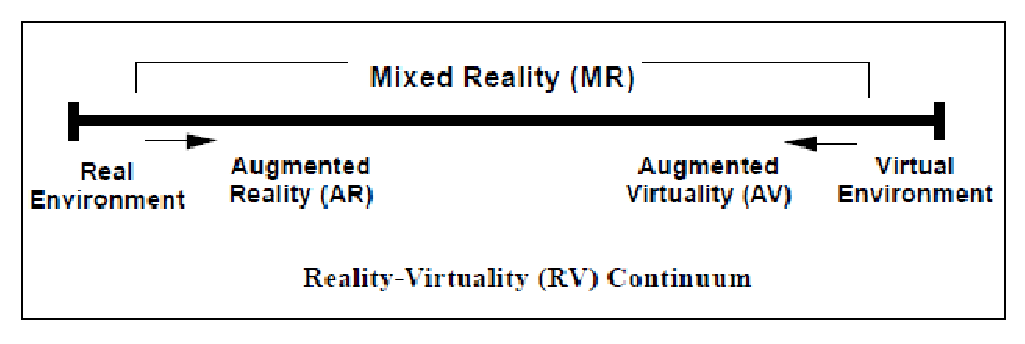
\includegraphics[width=6cm]{../../../img_ent1/reality_virtual.eps}
	\caption*{\tiny{Diagrama continuo de Realidad-Virtualidad. Milgram et al.}}
      \end{centering}
    \end{figure}
  \end{itemize}
\end{frame}

\begin{frame}{Sistemas y métodos para detección en RA}
    \begin{block}{Tipos de sistemas}
      \begin{itemize}
	    \item Basada en marcadores. \note[item]{es una imagen sintetica que altera el ambiente}
	    \item \textbf{No basada en marcadores} $\rightarrow$ características naturales de los objetos.
	      \note[item]{Marcelo: las características son de los objetos y NO DE LAS IMÁGENES}
      \end{itemize}
    \end{block}
   
     \begin{block}{Métodos para detección y seguimiento de objetos}
	\begin{itemize}
		\item Seguimiento basado en localización (GPS, acelerómetros, giroscopios, etc.)
		\item \textbf{Seguimiento óptico} $\rightarrow$ análisis e identificación de características a partir de la imagen.
		\item Una combinación de los dos anteriores.
	\end{itemize}
     \end{block}
\end{frame}

\begin{frame}{Aplicaciones - Ejemplos}
    \note[item]{Decir "marcadores" y  no patrónes!}
	\begin{center}{Aplicaciones - Ejemplos}
	  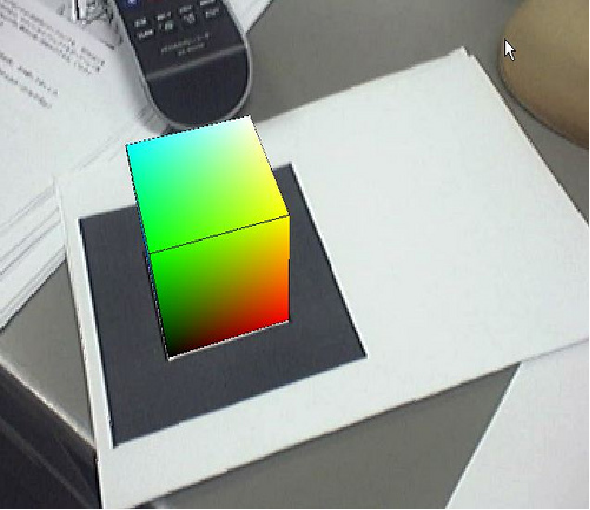
\includegraphics[width=7cm]{./img1/objeto_y_patron}
  	  
\includegraphics[width=7cm]{./img1/patrones}
	\end{center}
\end{frame}

\begin{frame}{Aplicaciones - Ejemplos}
      \note[item]{Decir "marcadores" y  no patrónes!}
	\begin{center}
	  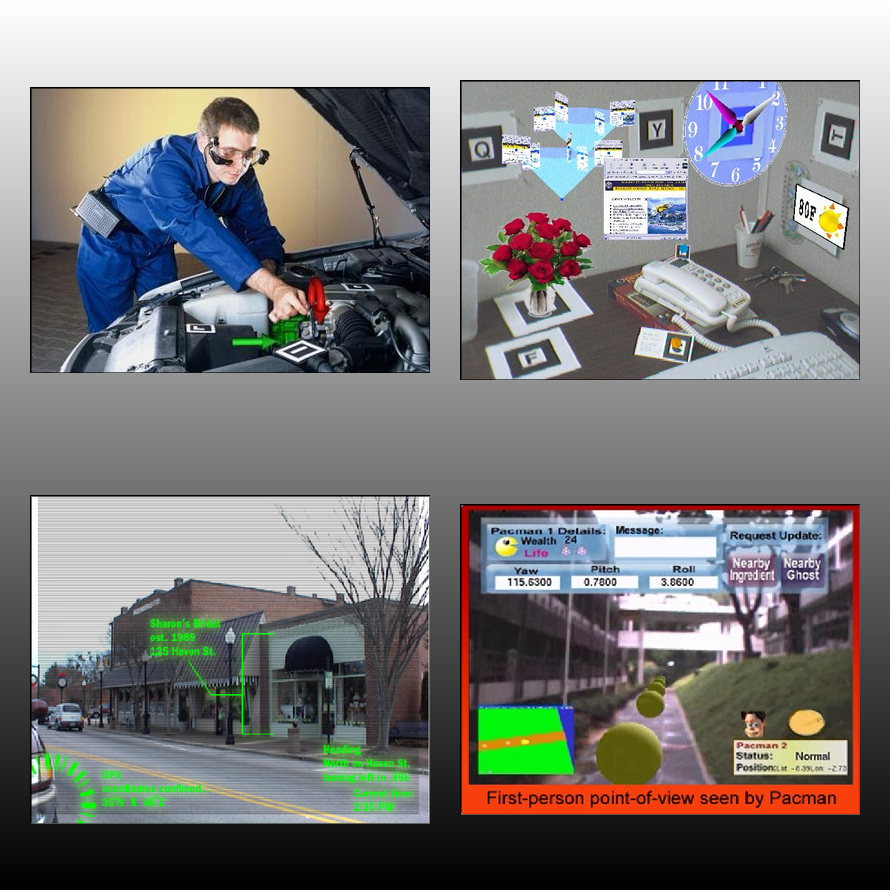
\includegraphics[width=7cm]{./img1/aplic1}
	\end{center}
\end{frame}
%%%%%%%%%%%%%%%%%%%%%%%%%%%%%%%%%%%%%%%%%%%%%%%%%%%%%%%%%
\subsection*{}
\begin{frame}{Motivación}
  \begin{itemize}
  \note[item]{Construir un método que permita reconocer objetos planos e identificar su posición en la imagen, en un ambiente controlado, para la posterior aplicación de realidad aumentada.}
  \item Desarrollo de un software propio de RA adaptable a aplicaciones específicas (comerciales, educativas, lúdicas, etc.)\footnote{SINC: Centro de Investigación en señales, sistemas e inteligencia computacional}
  \item No todas las aplicaciones trabajan en tiempo real.
  \item Muchos utilizan marcadores artificiales.
  \item Distribuidos bajo licencias privativas o costosos.
  \item Se trabaja con una tecnología que se encuentra en auge en estos tiempos.
      \note[item]{A cobrado gran imulso en el marketing, educación y e-commerce}
  \item El reconocimiento de objetos puede ser aplicado a diversidad de temáticas.
  \end{itemize}
\end{frame}

% \begin{frame}{Objetivos generales}
%   \begin{itemize}
%       \item Desarrollar un método para reconocer y seguir objetos en una secuencia de video digital y desarrollar un prototipo que haga uso del mismo aplicándolo a realidad aumentada.
%       \item Afianzar y extender los conocimientos adquiridos en el cursado de la carrera Ingeniería en Informática.
%   \end{itemize}
% \end{frame}
\subsection*{}
\begin{frame}
  \frametitle{Objetivos}
    \begin{itemize}
% 	\item Realizar el relevamiento del estado del arte en métodos utilizados para la detección y seguimiento de objetos en el Procesamiento Digital de imágenes.
	\item Diseñar y desarrollar un método reconocedor y seguidor de objetos planos en el flujo de video tomado por una cámara web estándar, sobre un ambiente controlado.
	\item Implementar el método en un algoritmo computacional que sea multiplataforma.
	%\item Optimizar el procesamiento llevado a cabo para lograr método desarrollado para que sea aplicable en tiempo real (\textbf{procesamiento}). 
	\item Optimizar el procesamiento para aplicarlo en tiempo real. 
	\item Implementar una aplicación prototipo específica (en el área de turismo, educación, publicidad, juegos u otros).
    \end{itemize}
\end{frame}

% \begin{frame}
% \frametitle{Alcances}
% \begin{itemize}
%   \item Se enmarcará en un sistema del tipo \textbf{sin marcadores} con método de reconocimiento del tipo \textbf{seguimiento óptico}.
%   \item El proyecto involucra el desarrollo de un prototipo para ser utilizado en una computadora con una cámara web estándar. Cabe aclarar, que no se pretende realizar una aplicación final específica y completa (estudio y diseño de interfaz amigable al usuario, introducción amigable de parámetros, etc.) orientada al uso de un usuario final.
%   \item Aunque no es un objetivo la implementación de varios métodos y su comparación, en una etapa previa se revisarán las características de algunos métodos para poder seleccionar alguno que se adecue a los requerimientos.
% \end{itemize}
% \end{frame}
%%
     \section{Método propuesto}
\subsection*{}
\begin{frame}{Detección de objetos} % o puntos característicos y descriptores?
  \begin{itemize}
  \item Buscar en una imagen o un video (secuencia de imágenes) un objeto particular dado.
      \note[item]{El reconocimiento de objetos se puede resumir en el objetivo de }
      \note[item]{de forma que estos permitan distinguirla de otras sin la necesidad de tener que analizar la totalidad de la imagen.}
  \item Seleccionar algunos puntos como características distintivas del objeto en la imagen.
    \note[item]{Marcelo: Una de las formas de hacer esto es mediante la detección de puntos claves....* OJO EXISTEN OTRAS FORMAS DE DETECTAR LOS OBJETOS NO SOLO MEDIANTE PUNTUALES... UNA FORMA....}
    \note[item]{(una cantidad suficiente) que sean distinguibles, estables, posean repetibilidad y puedan localizarse.}
    \note[item]{Cuando se tienen imágenes de una misma escena, las correspondencias 2D pueden ser extraídas en cada fotograma para estimar la posición del objeto buscado mediante la identificación de puntos característicos naturales,}
    \note[item]{Una característica local puede ser interpretada como un patrón de imagen que difiere de su vecindad}
    \note[item]{puede venir representada por ejemplo por un punto, un borde o pequeños trozos de la imagen}
  \item La búsqueda de estos puntos, se puede realizar mediante detectores de puntos claves.
  \item Se representa la vecindad de cada punto de interés detectado mediante un vector descriptor.
      \note[item]{Es común la realización de ciertos cálculos sobre una región alrededor de la característica local detectada y su resultado se convierte en un vector numérico el cual recibe el nombre de descriptor}
      \note[item]{Idealmente, este descriptor debe ser distintivo, robusto al ruido, a la detección de desplazamientos y a las deformaciones geométricas o fotométricas de la imagen.}
  \item Se buscan las correspondencias entre los vectores descriptores de las imágenes. 
    \note[item]{La dimensión del descriptor impacta directamente en el tiempo de cálculo y distintividad.}
    \note[item] {Estos detectores son la base de gran cantidad de herramientas basadas en visión computacional(reconocimiento de objetos, vigilancia por video, imágenes médicas, la realidad aumentada, etc.)} 

\note[item]{Características locales: Cuando se trabaja con características locales uno de los primeros inconvenientes a resolver es obtener un alto nivel de invarianza: esto depende de las deformaciones geométricas y fotométricas que pueda sufrir la imagen.
 \begin{itemize}
  \item Nos centraremos en: cambios de escala, la rotación en el plano,
  \item Se asume que los efectos de segundo orden: inclinación, perspectiva y anisotropía son cubiertos en cierto grado por la robustez global del descriptor utilizado
  \item En cuanto a las deformaciones fotométricas, se asume un modelo lineal simple con un desplazamiento y un cambio de contraste (factor de escala).
 \end{itemize}
}
% \subsection{Realidad Aumentada}
  \end{itemize}
\end{frame}
\subsection*{Método}
\subsubsection*{Etapas}
\begin{frame}{Etapas}
\note[item]{El método propuesto posee 2 etapas}
  \begin{block}{Configuración}
   \begin{itemize}
    \item Se realiza una sola vez al inicio del algoritmo.
    \item Se registra la imagen que posteriormente se detectará en el flujo de video.
   \end{itemize}
  \end{block}
  \begin{block}{Ejecución}
	\note[item]{Marcelo: 
	  aplique condicionales
	  se resuelven incongruencias en transformaciones
	  aumenta la velocidad de procesamiento
	  resulta sin flickering
	}
   \begin{itemize}
    \item Captura de un frame del flujo de video proporcionado por la cámara web.
    \item Procesamiento para detectar el objeto registrado en la Configuración.
    \item Superposición de un objeto virtual para enriquecer la realidad.
   \end{itemize}
  \end{block}
\end{frame}
%
\begin{frame}{Etapa de configuración}
	\begin{center}
  	  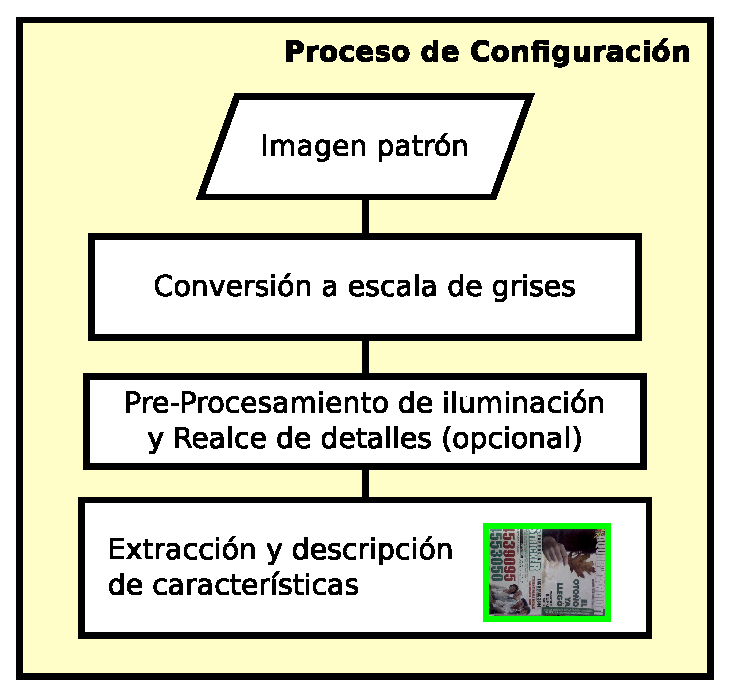
\includegraphics[scale=0.5]{../../figs/proceso_completo_entrenamiento_presentacion}
	\end{center}
\end{frame}
%
\begin{frame}{Etapa de ejecución}
	\note[item]{Marcelo: antes de explicar etapa 2: decir que hace el método estandar. Existe un método.. o algo asi...}
	\begin{center}
  	  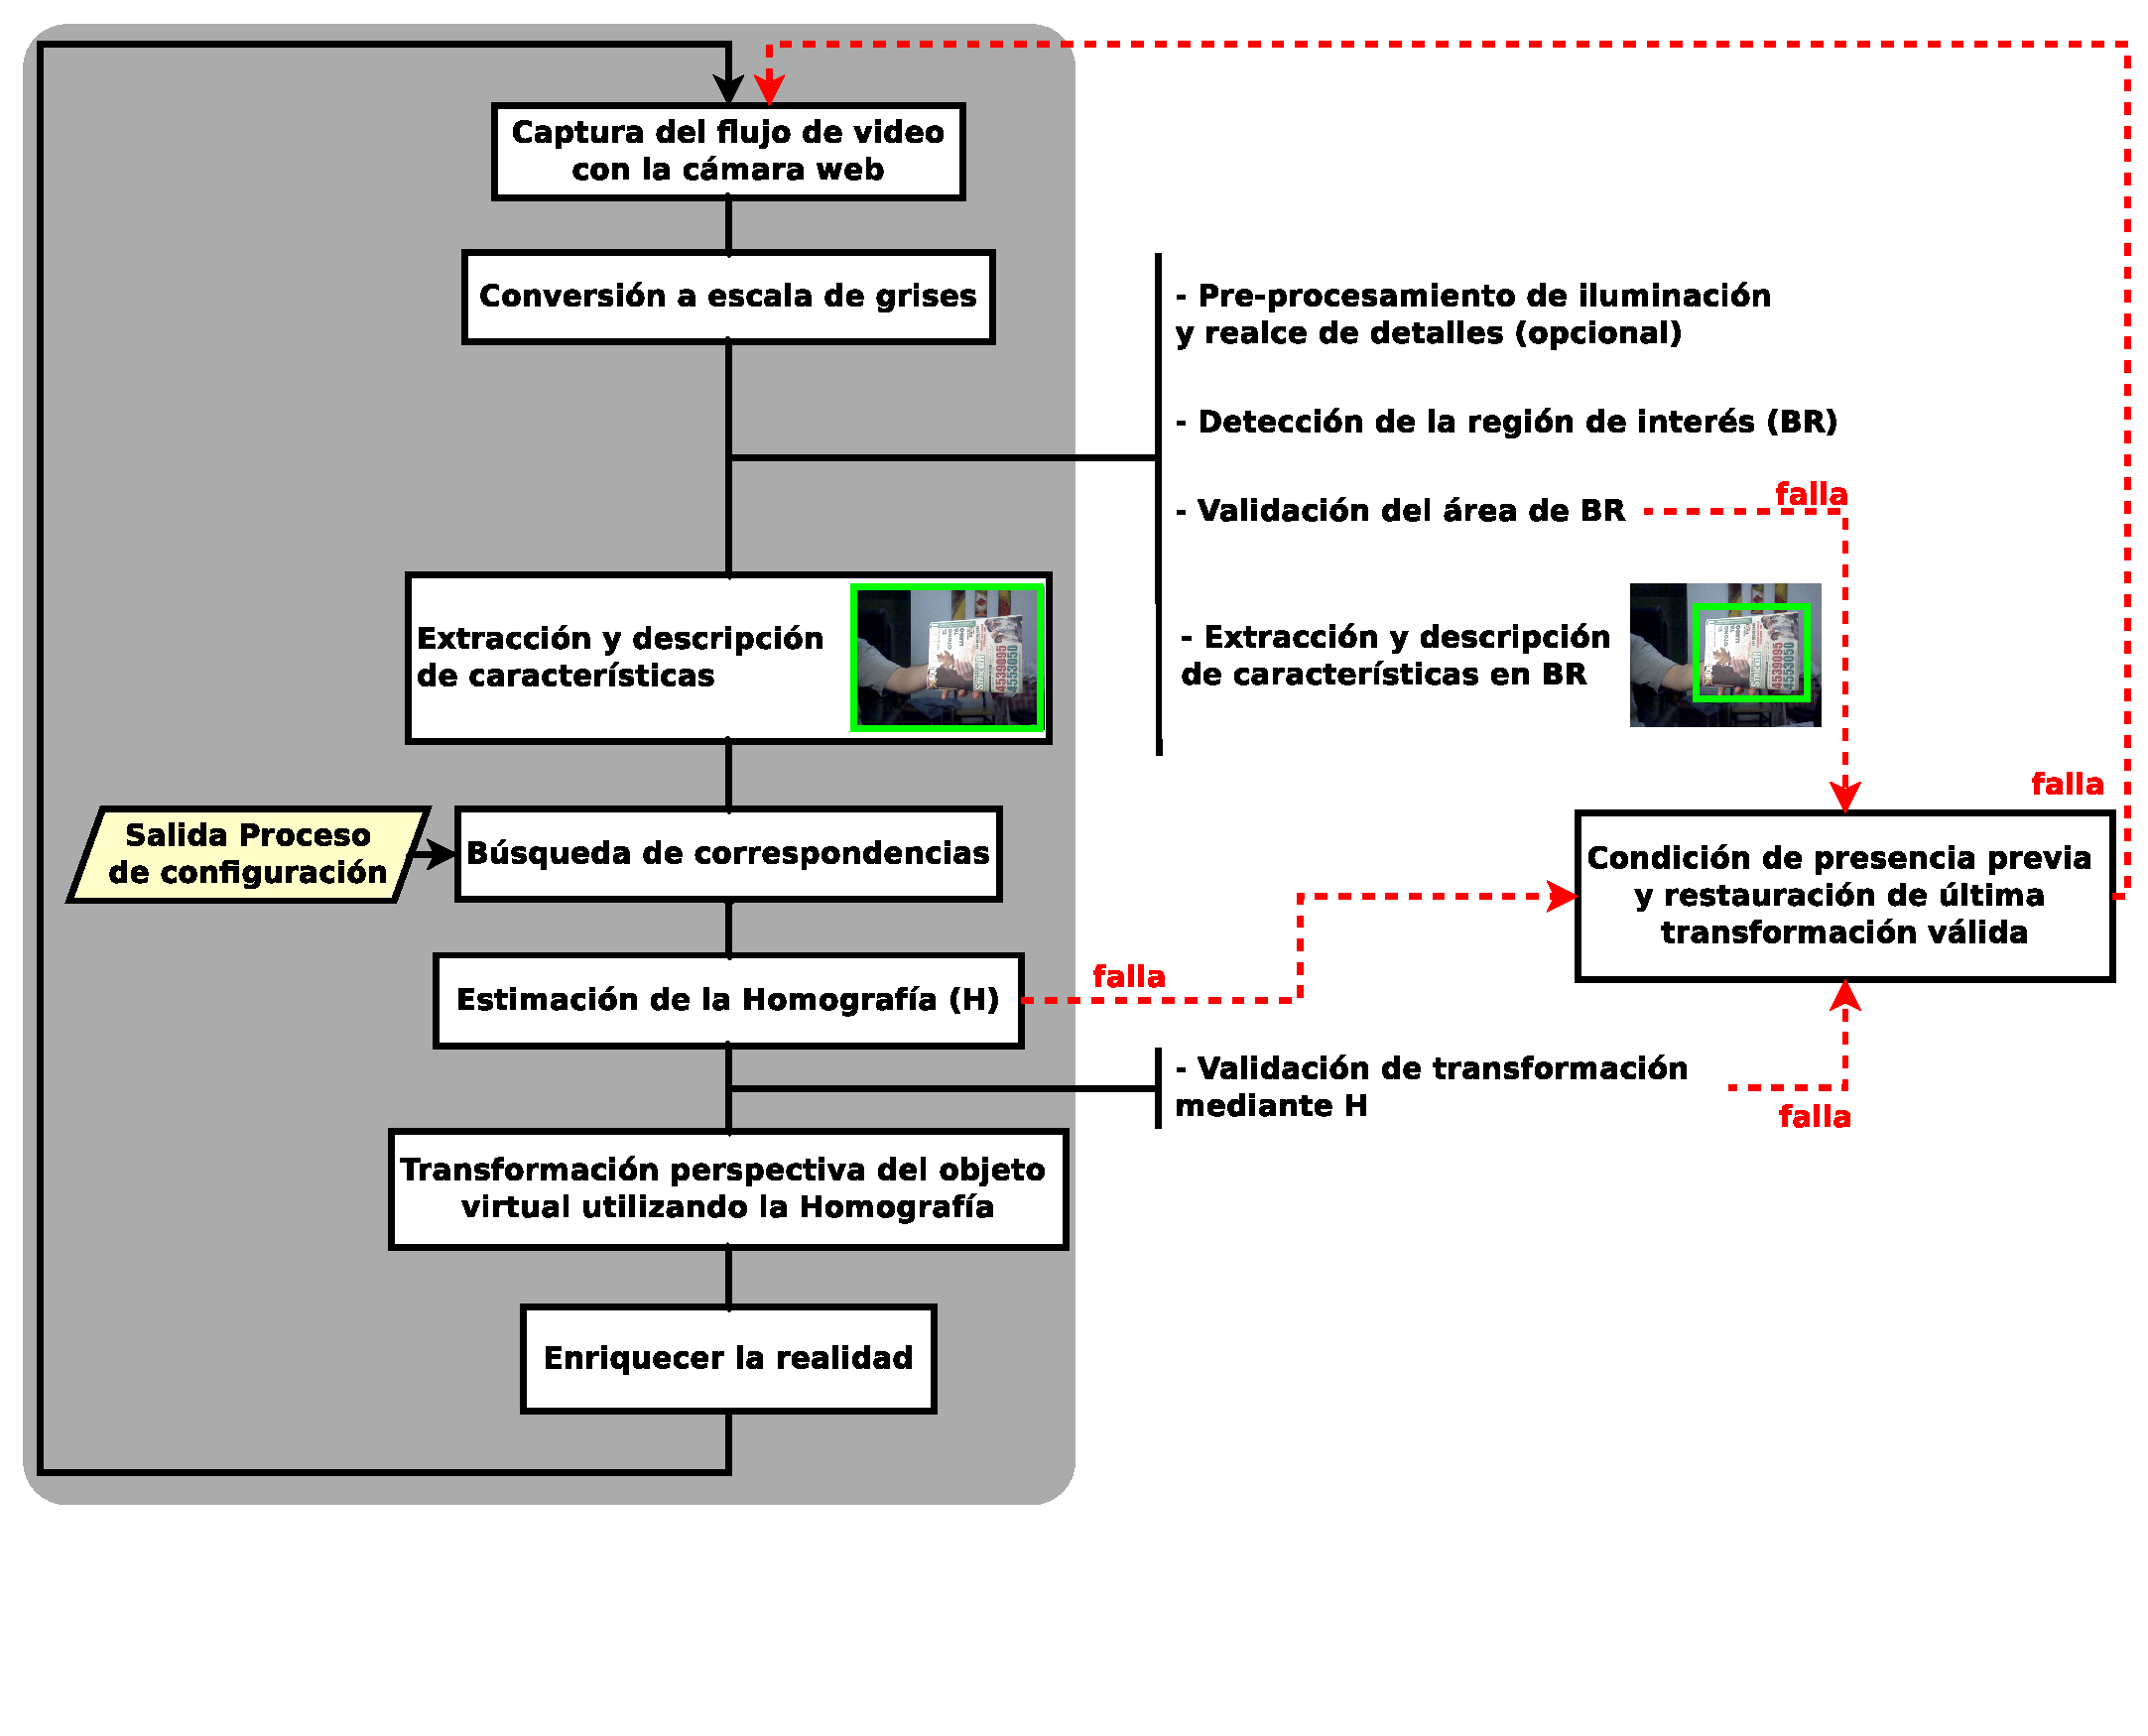
\includegraphics[scale=0.29]{../../figs/proceso_completo_presentacion_negrita} %proceso_completo_presentacion1
	\end{center}
\end{frame}

% \begin{frame}{Etapa de ejecución}
%     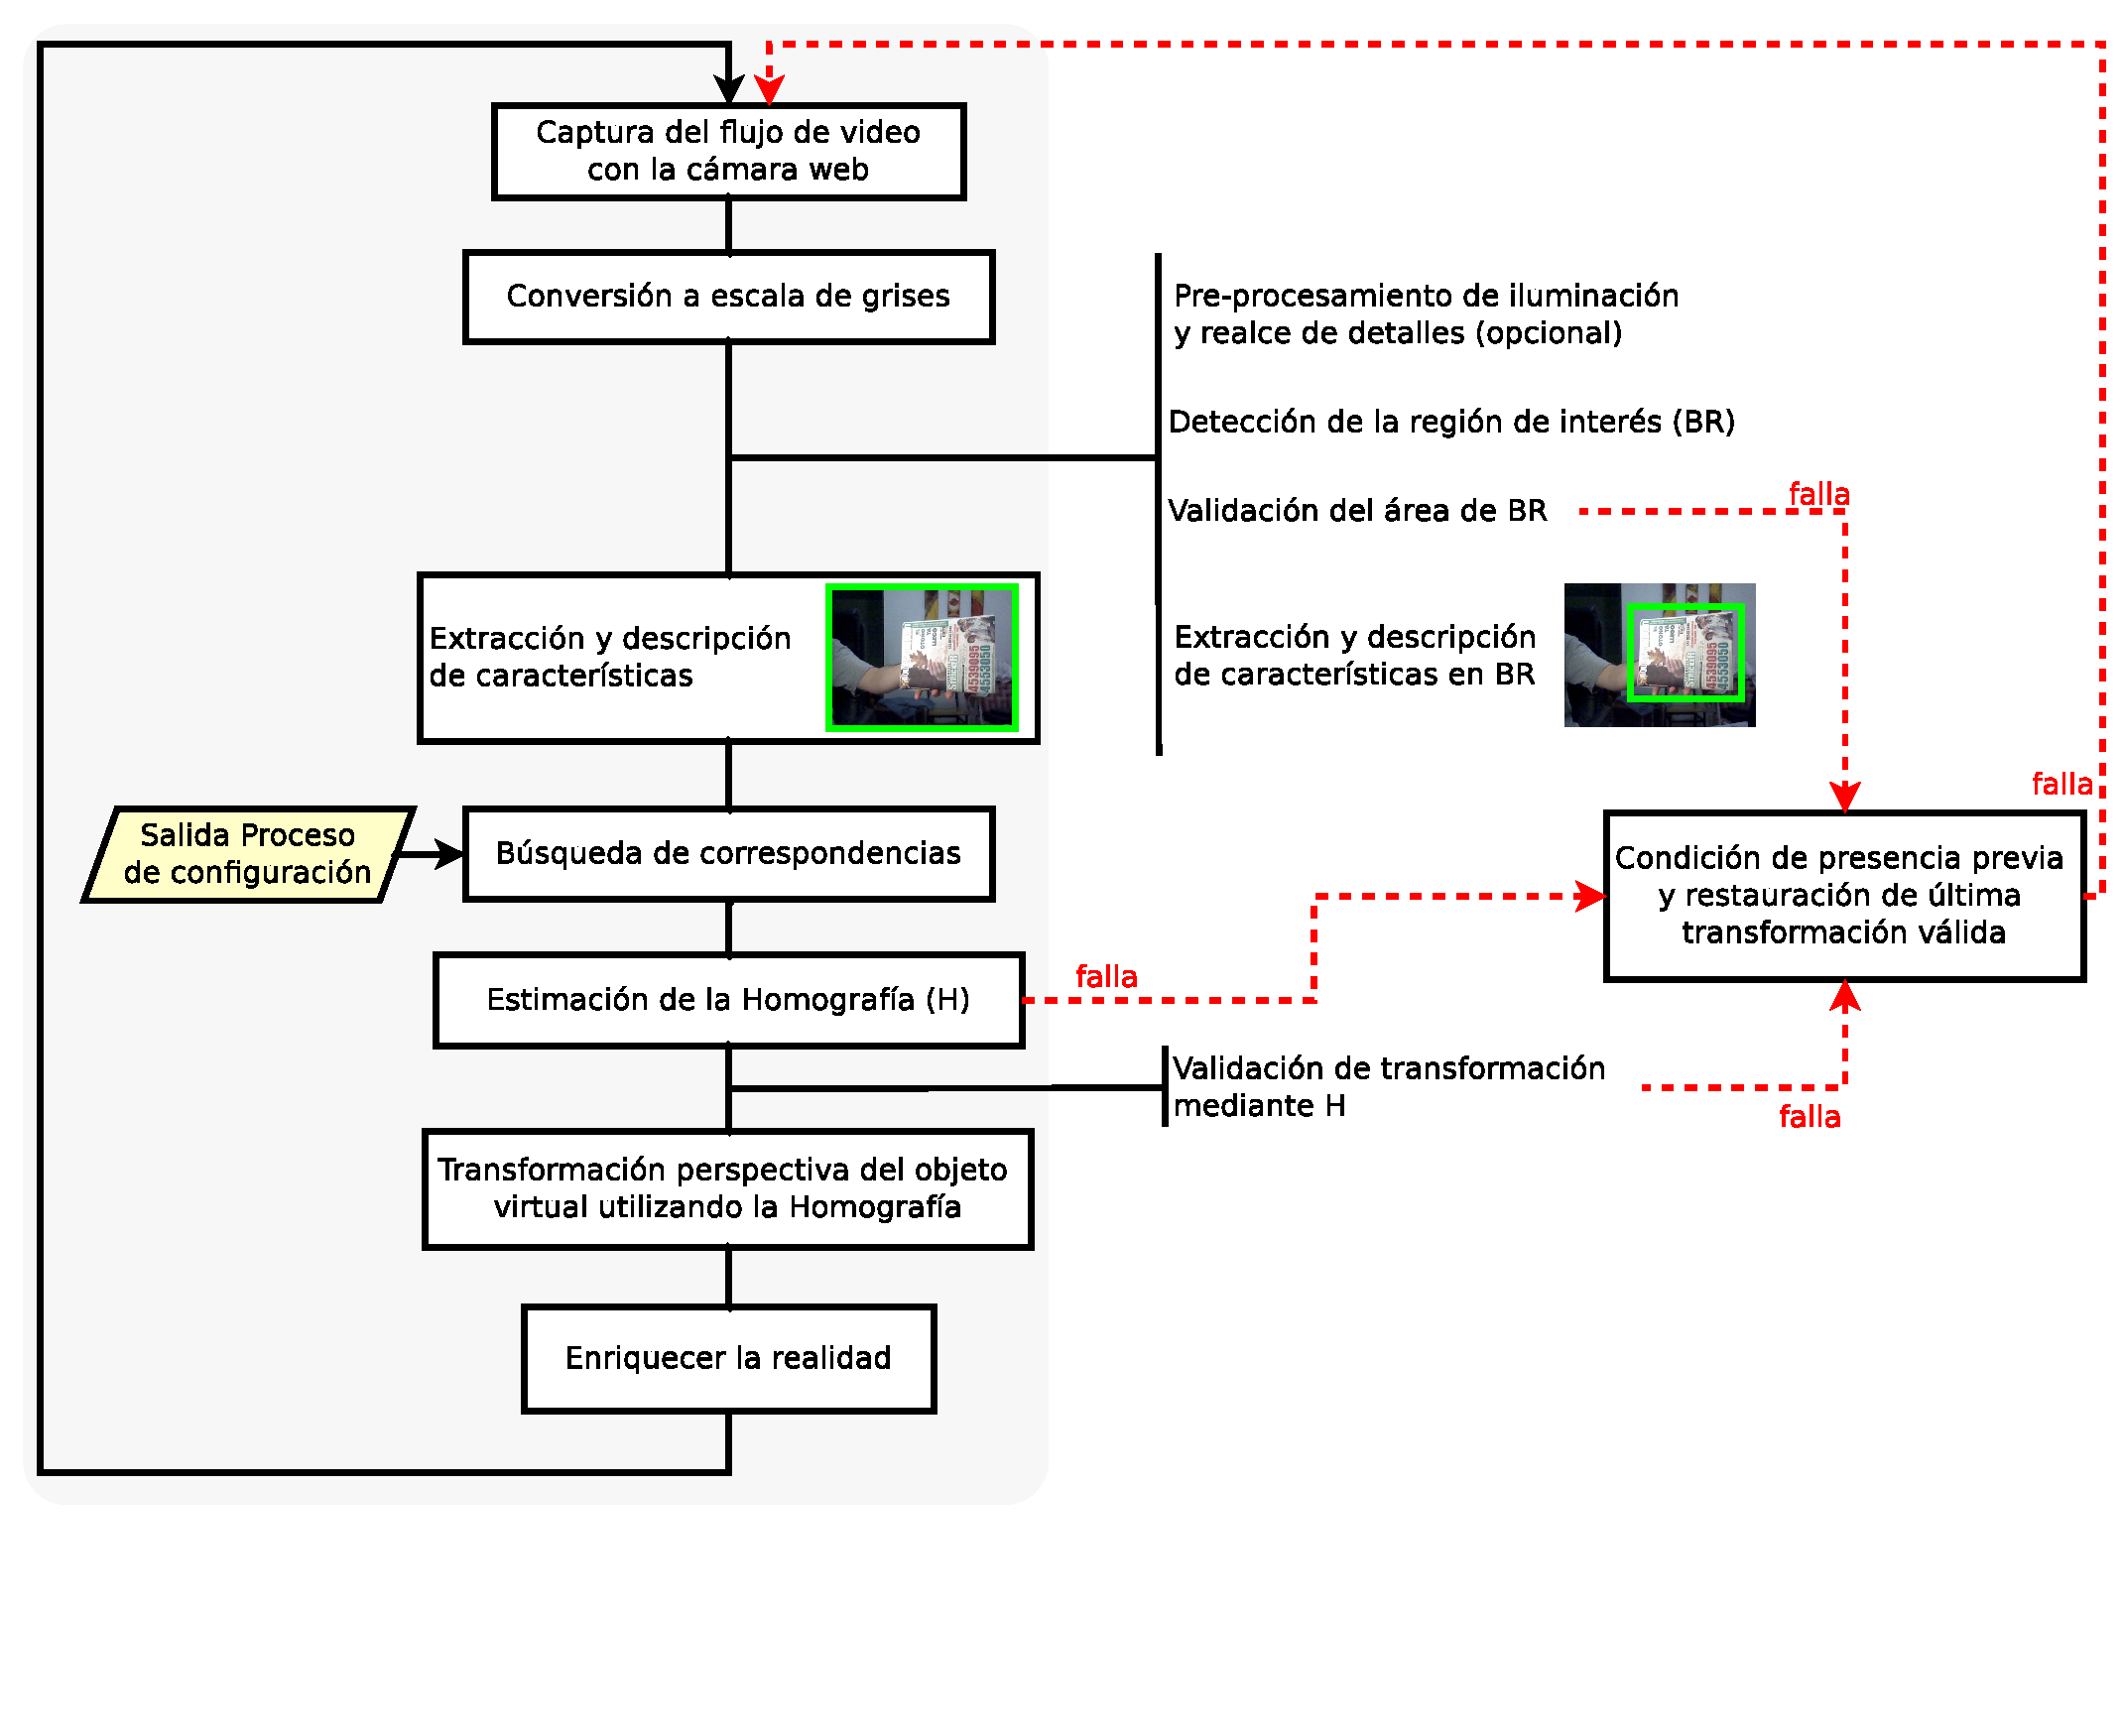
\includegraphics[scale=0.2]{../../figs/proceso_completo_presentacion}
%     \framezoom<1><1>[border](0cm, 0cm)(2.5cm, 3.4cm)
% \end{frame}
% \begin{frame}{Etapa de ejecución}
%     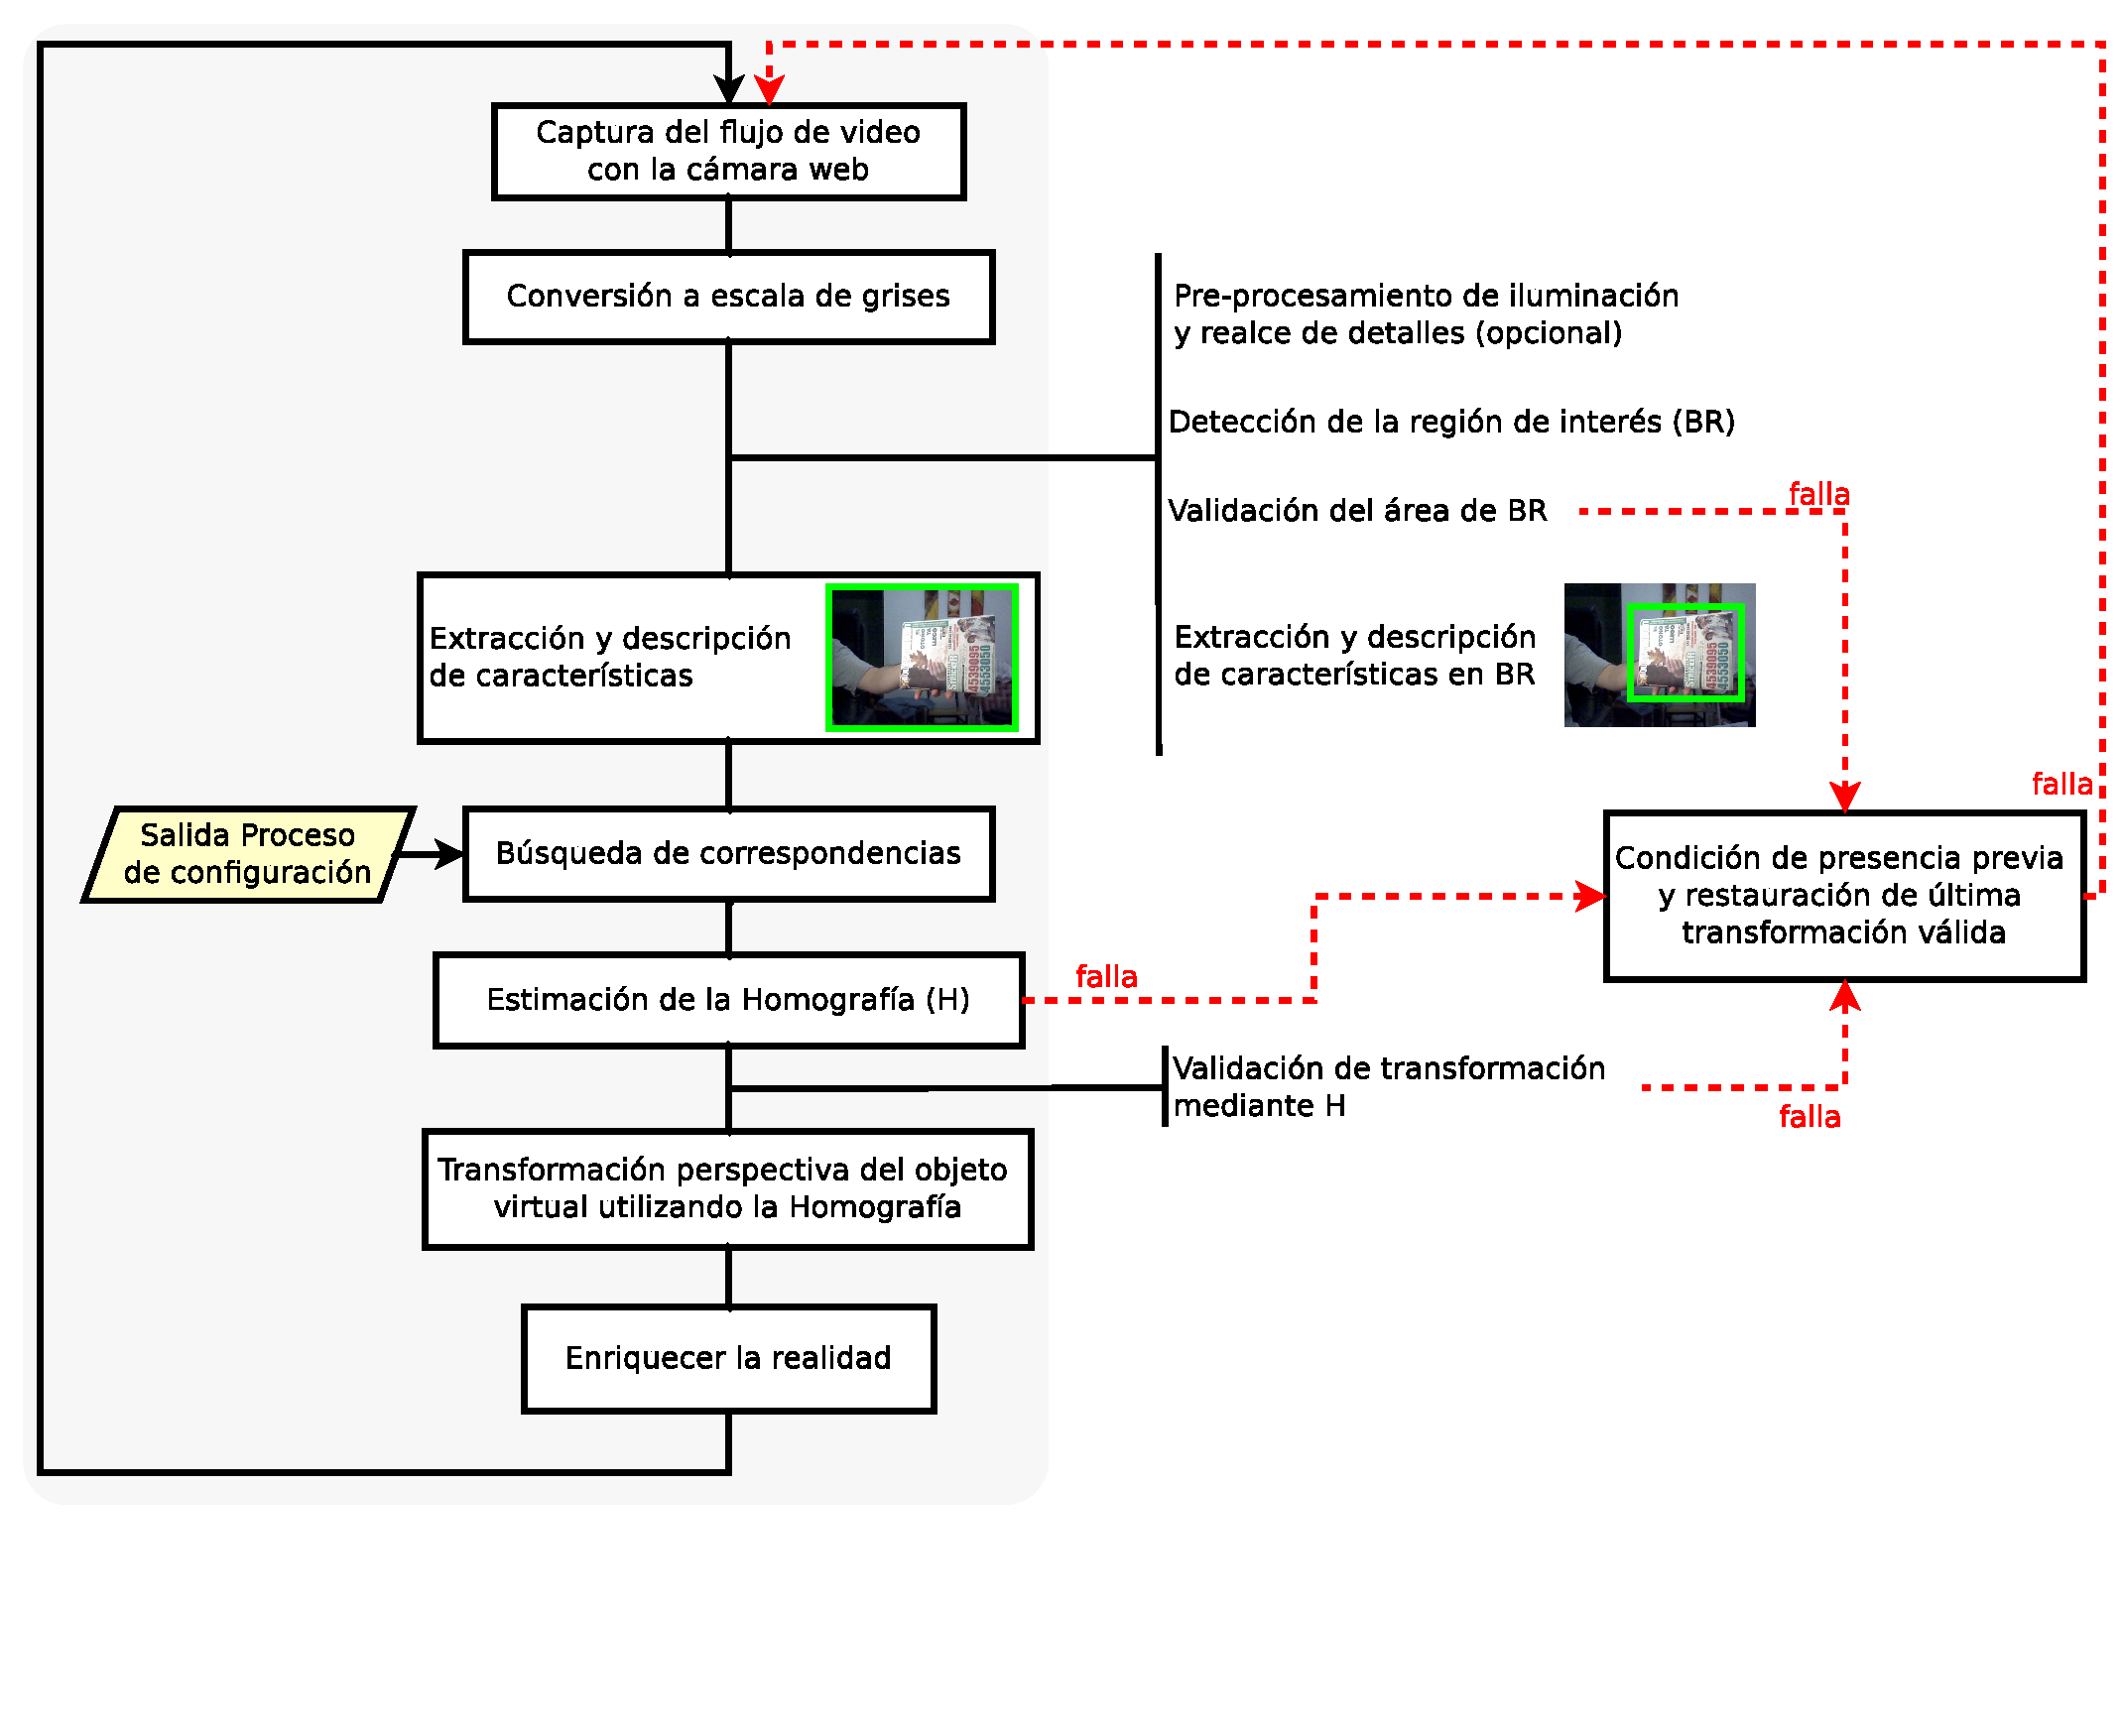
\includegraphics[scale=0.2]{../../figs/proceso_completo_presentacion}
%     \framezoom<2><1>[border](0cm, 3.4cm)(3cm, 3.4cm)
% \end{frame}

\subsection*{}
\begin{frame}{Conversión a escala de grises}
	Formula perceptualmente ponderada:
	\begin{equation*}
	  \label{eq:formula_conv_grises}
	  I=0.299R+0.587G+0.114B.
	\end{equation*}
\end{frame}

\begin{frame}{Pre-procesamiento de realce de detalles y mejora en iluminación}
    \begin{itemize}
      \item Transformación logarítmica 
	$\hspace{0.2cm}
	  s=\;log(1+r) 
	  \label{eq:logaritmo}
	$.
	\note[item]{utilizada cuando la imagen de entrada tiene un rango dinámico grande, expande las intensidades oscuras y comprime las intensidades claras... Los oscuros se ven mas claros y los claros aún mas claros}
      \item Ecualización del histograma.
	\note[item]{Es una función que describe de manera global la apariencia de una imagen. Puede interpretarse como el número de píxeles en función de las intensidades de grises.}
	\note[item]{Pretende obtener el mismo número de píxeles para cada nivel de gris (distribución que se aproxima a la uniforme).}
	\note[item]{Se obtiene una expansión en el rango dinámico de la imagen - aumento del contraste.}
      \item Filtrado pasa altos: \note[item]{realza las altas frecuencias - realza los detalles}
	\note[item]{puede ser aplicado mediante la convolución de la imagen con un kernel pasa altos. Si la suma de los coeficientes del kernel es 1, se realzan las altas frecuencias conservándose el brillo medio de la imagen sobre la cual se aplica el filtro.}
	\small{
	\begin{equation*}
	  g(x,y)=\sum_{s=-a}^{a}\sum_{\; t=-b}^{a}w(s,t)f(x+s,y+t)\label{eq:ec_convolucion}
	  \hspace{0.2cm}
	  w=\begin{bmatrix}
	  \quad0 & -1 & \quad0\\
	  -1 & \quad5 & -1\\
	  \quad0 & -1 & \quad0
	  \end{bmatrix}
	\end{equation*}}
	 \item Filtrado de alta potencia: 
	      \note[item]{se obtiene entre una versión amplificada de la imagen original y una versión suavizada de la misma}
	      \small{\begin{equation*}
		\label{eq:form_alta_potencia}
		g(x,y)=(A-1)f(x,y)+PA(f(x,y)) \hspace{0.2cm} \textrm{con} \hspace{0.2cm} A=2;
		\hspace{0.2cm} kernel=\begin{bmatrix}
		-1 & -1 & -1\\
		-1 & \quad8 & -1\\
		-1 & -1 & -1
		\end{bmatrix}
	      \end{equation*}
	    }
	    \note[item]{Formula equivalente: Af\-PB(f)}
      \item Ecualización del histograma y posteriormente filtrado de alta potencia.
	  \note[item]{Realzar el contraste y luego mejora los detalles}
    \end{itemize}
  \end{frame}
  
\subsection{Detección de movimiento}
\begin{frame}{Detección de la región de interés}
  Determinación de una zona de interés para realizar la extracción de características. 
    \note[item]{La región de interés es la parte cambiante del flujo de video}
	\begin{itemize}
		\item Diferencia de imágenes ($F$: cuadro del flujo de video).
		\begin{equation*}
		  D(x,y)=|F_{t}(x,y)-F_{t-1}(x,y)|\;\forall\; x,y\;\in F.
		  \label{eq:diferencia_absoluta}
		\end{equation*} \note[item]{La diferencia no es exacta, y aparece ruido y patrones speckle en la imagen}
		\item Umbral Binario.
		  \note[item]{Marcelo: no explicar umbral de binarización}
		  \note[item]{r y s son variables que denotan el nivel de gris.}
% 		$s=T(r)$
% 		\begin{equation*}
% 		  \label{eq:equation_umbral_binario}
% 		  s= 
% 		  \begin{cases} 0 & \text{para $r<50$,}
% 		  \\
% 		  255 &\text{para $r>=50$}
% 		  \end{cases} \textrm{con } 0 \leq r \leq 255% \textrm{ y } 0 \leq u \leq r_{max}.
% 		\end{equation*}
		\item Erosión $\times$ 2 $\rightarrow$ eliminar puntos aislados. \note[item]{eliminar detalles irrelevantes de una imagen binaria. El tamaño de los objetos se ve reducido y el ruido o detalles irrelevantes es eliminado.}
		\item Dilatación $\times$ 2 $\rightarrow$ recuperar eliminación de objetos de interés. \note[item]{los objetos crecen en su tamaño y algunos de los espacios dentro de ellos son rellenados}
		\item Rectángulo delimitador mínimo (BR).
		    \note[item]{$\rightarrow$ rectángulo más pequeño que encierra todos los puntos con valor diferente de 0.}
		\item Umbral sobre el área de BR
	\end{itemize}
\end{frame}

% \begin{frame}{Erosión y dilatación}
% 	\begin{itemize}
% 		\item Erosión $\rightarrow$ En una imagen erosionada, el tamaño de los objetos se ve reducido y el ruido o detalles irrelevantes (aislados) es eliminado
% 		\item Dilatación $\rightarrow$ los objetos crecen en su tamaño y algunos de los ``espacios'' dentro de ellos son rellenados (complementaria a la Erosión)
% 	\end{itemize}
% 		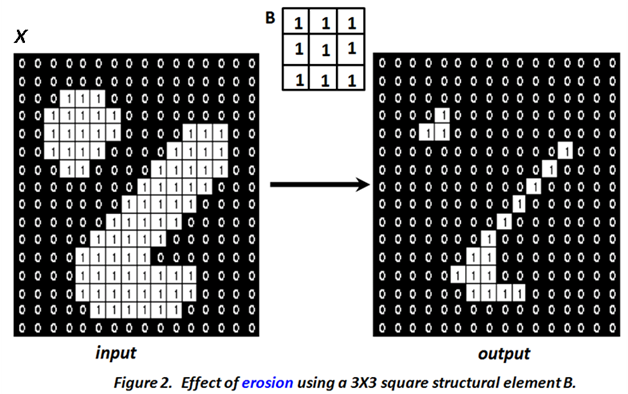
\includegraphics[width=5cm]{./img1/erosion}\qquad
% 		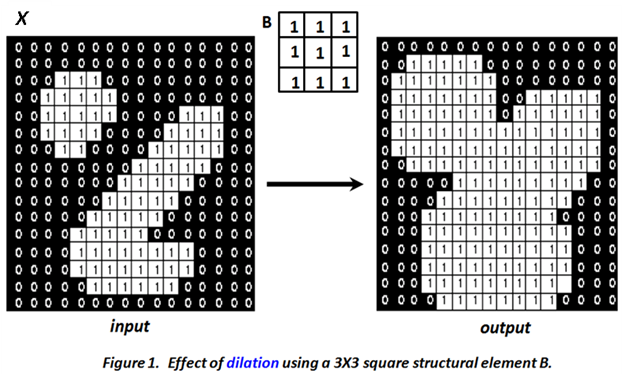
\includegraphics[width=5cm]{./img1/dilation}
% \end{frame}

\begin{frame}{Detección de la región de interés}
  \begin{figure}[tbhp]
    \centering
    \subfloat[][\small{Frame Previo}]{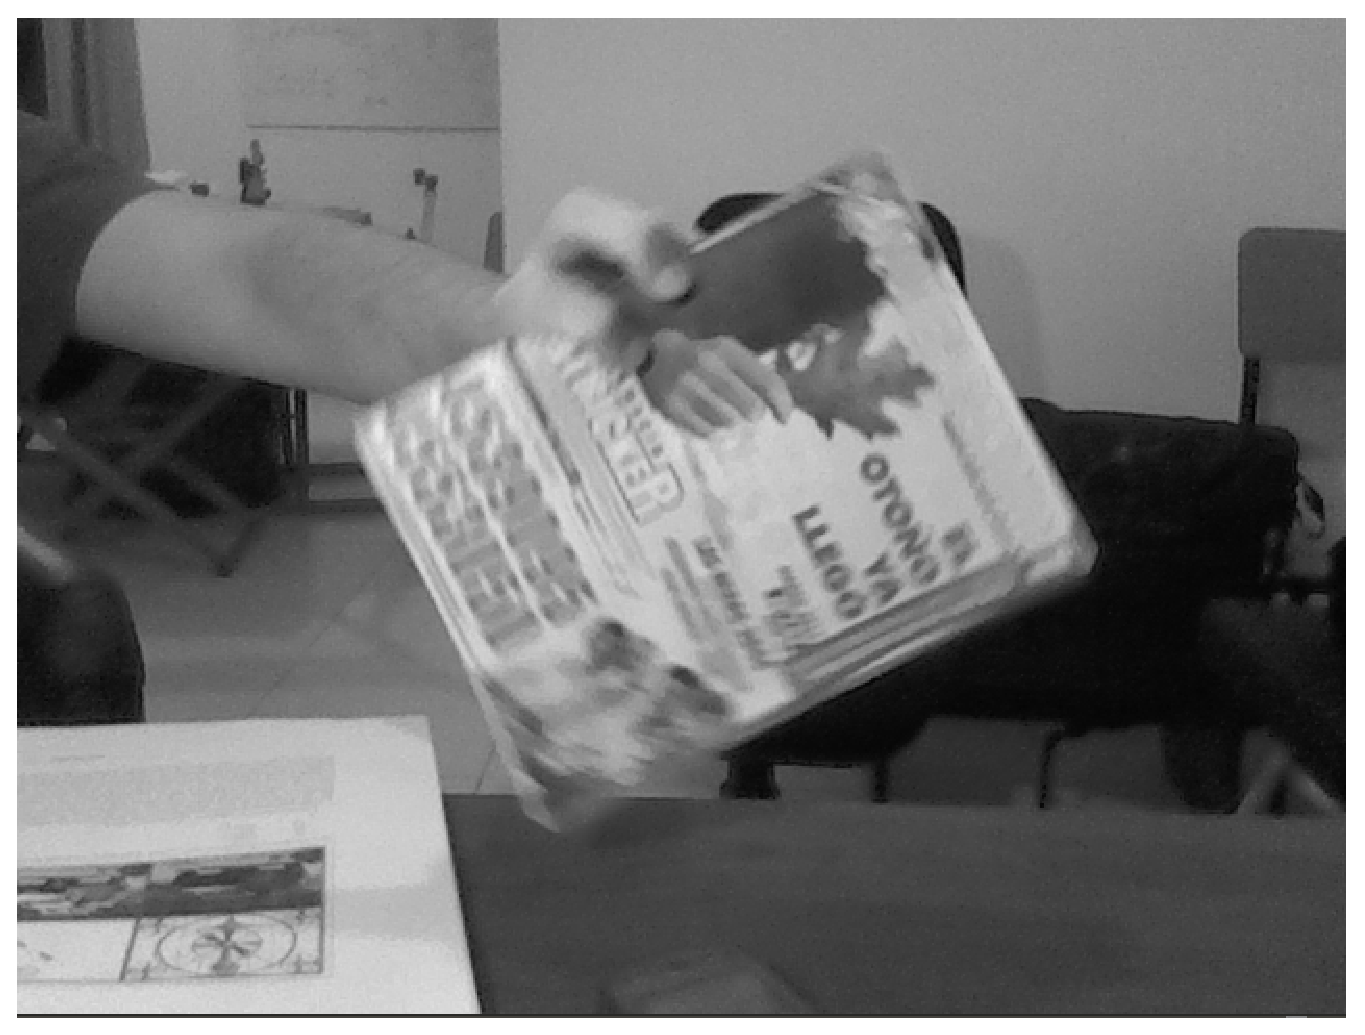
\includegraphics[width=0.27\textwidth]{../../figs/preprocess/srcPrev} \label{fig:deteccion_movimietno-srcprev}}
    \subfloat[][\small{Frame Actual}]{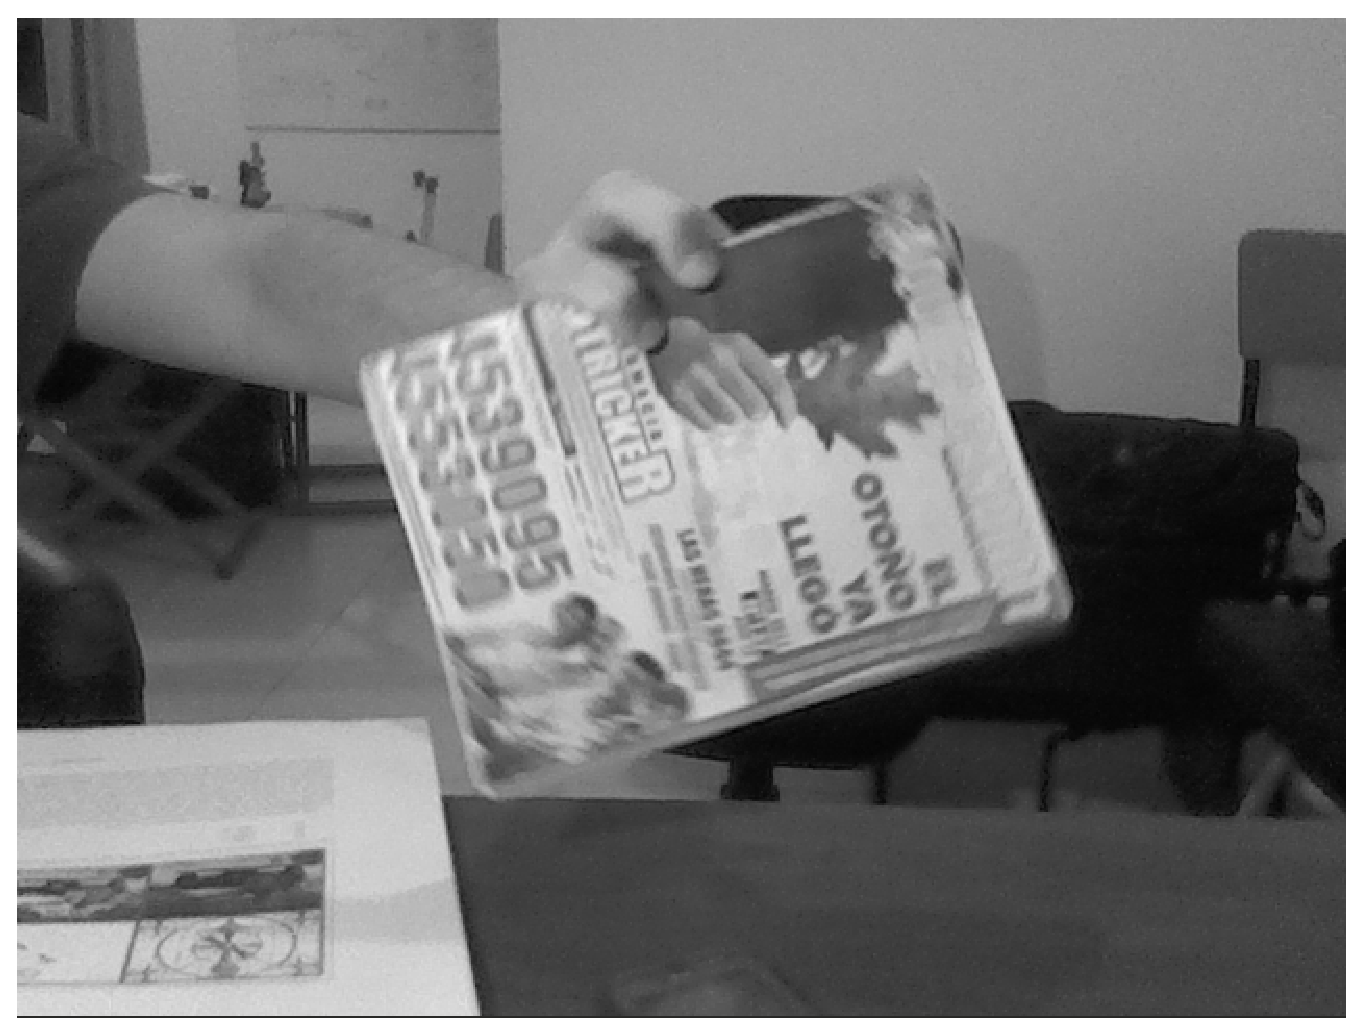
\includegraphics[width=0.27\textwidth]{../../figs/preprocess/src} \label{fig:deteccion_movimietno-src}}
    \subfloat[][\small{Diferencia absoluta}]{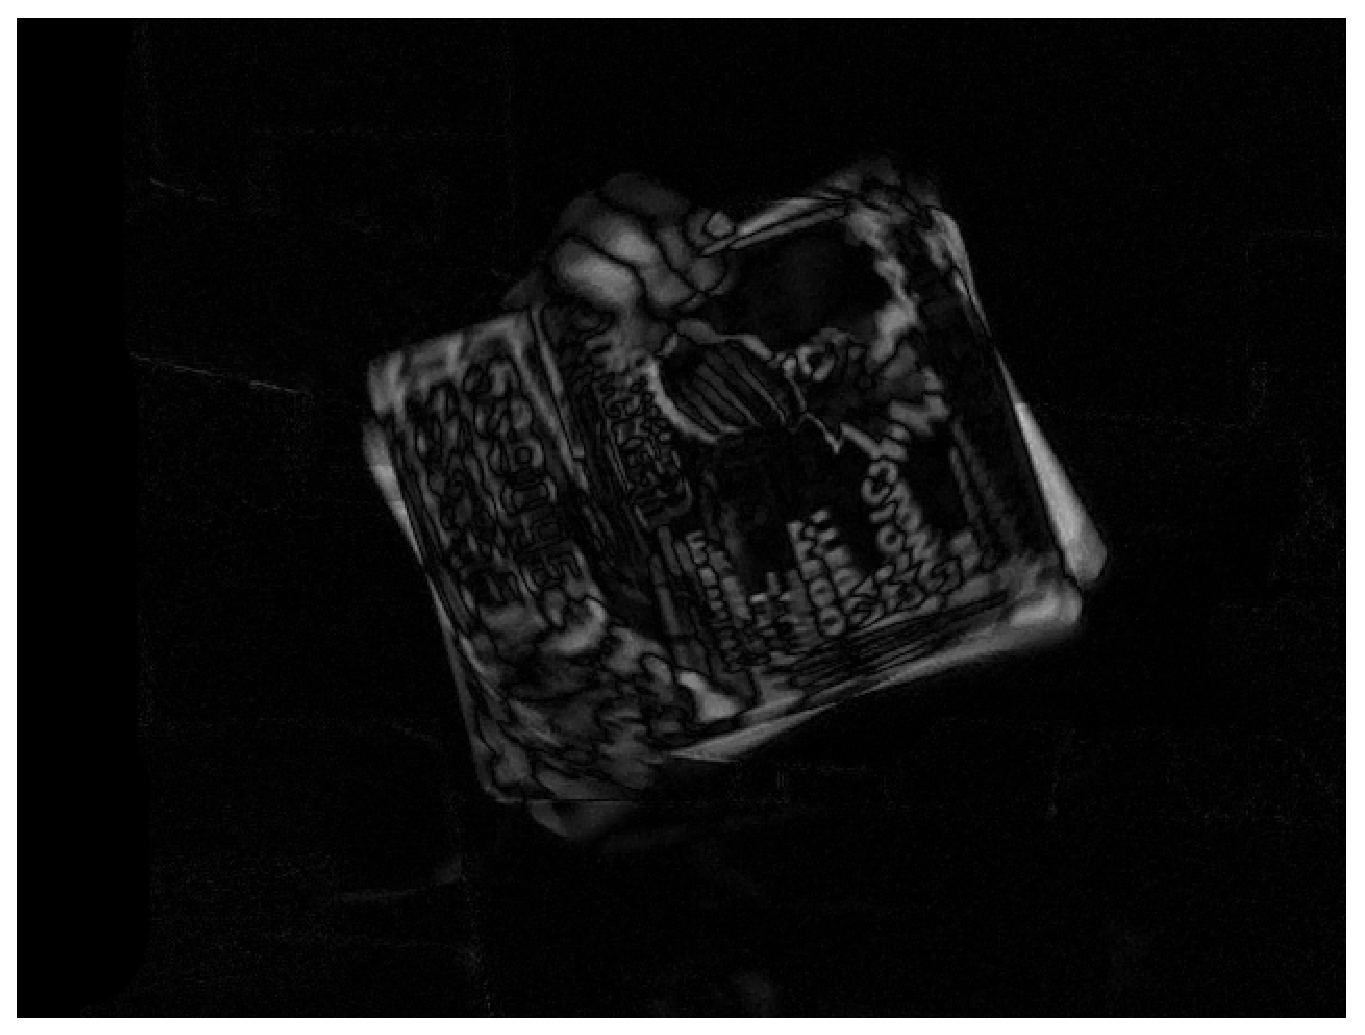
\includegraphics[width=0.27\textwidth]{../../figs/preprocess/absDiff} \label{fig:deteccion_movimietno-absdiff}}
    \subfloat[][\small{Umbral binario}]{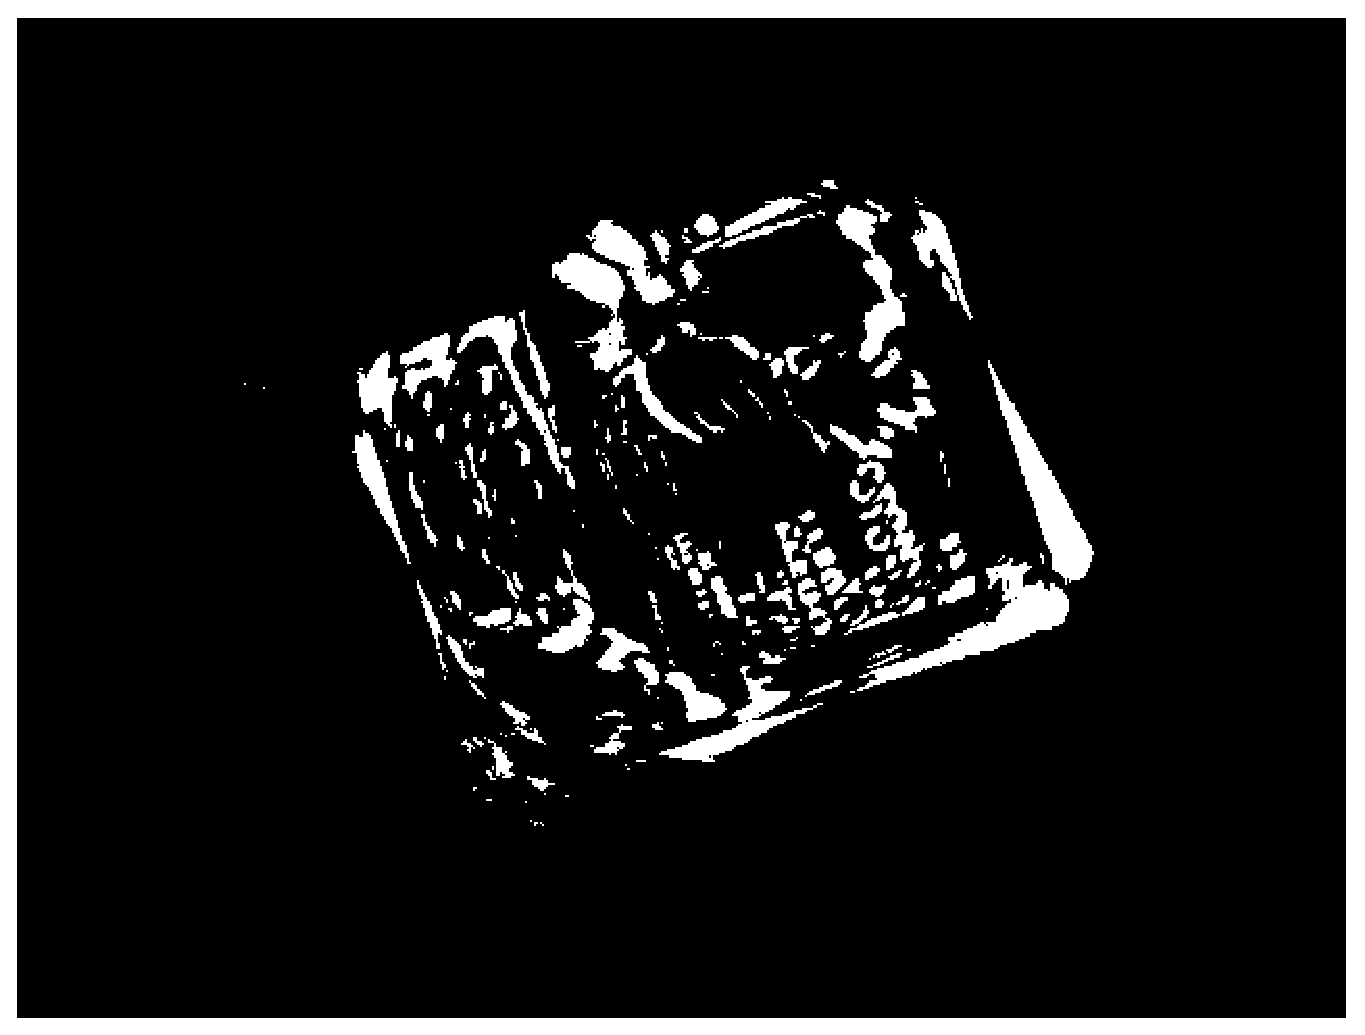
\includegraphics[width=0.27\textwidth]{../../figs/preprocess/threshold} \label{fig:deteccion_movimietno-umbral}}\\
    \subfloat[][\small{Erosión $\times2$}]{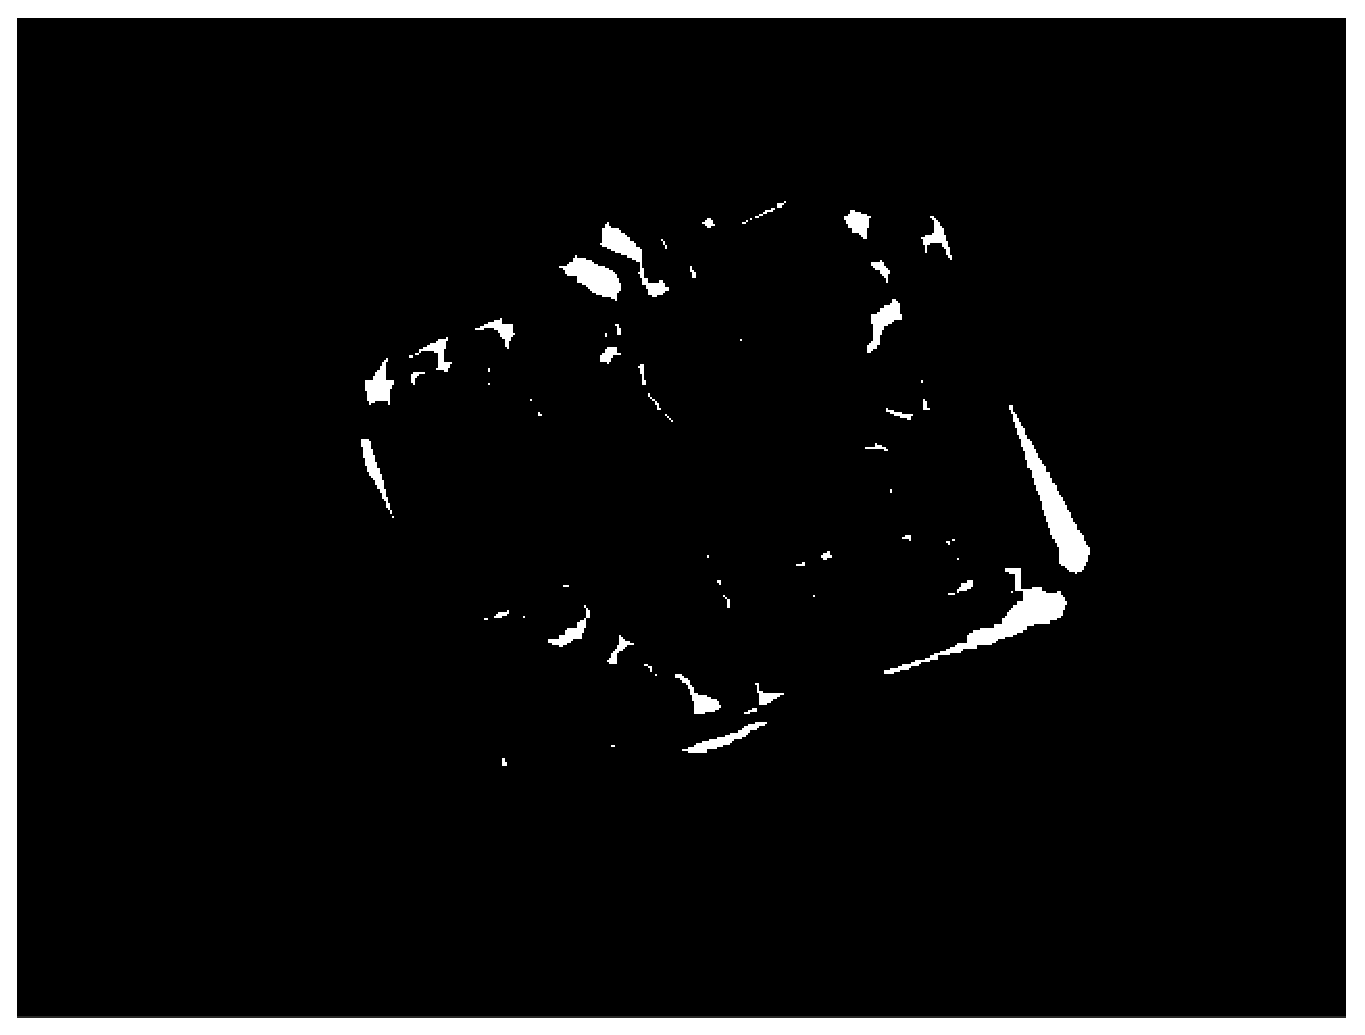
\includegraphics[width=0.27\textwidth]{../../figs/preprocess/erode} \label{fig:deteccion_movimietno-erode}}
    \subfloat[][\small{Dilatación $\times2$}]{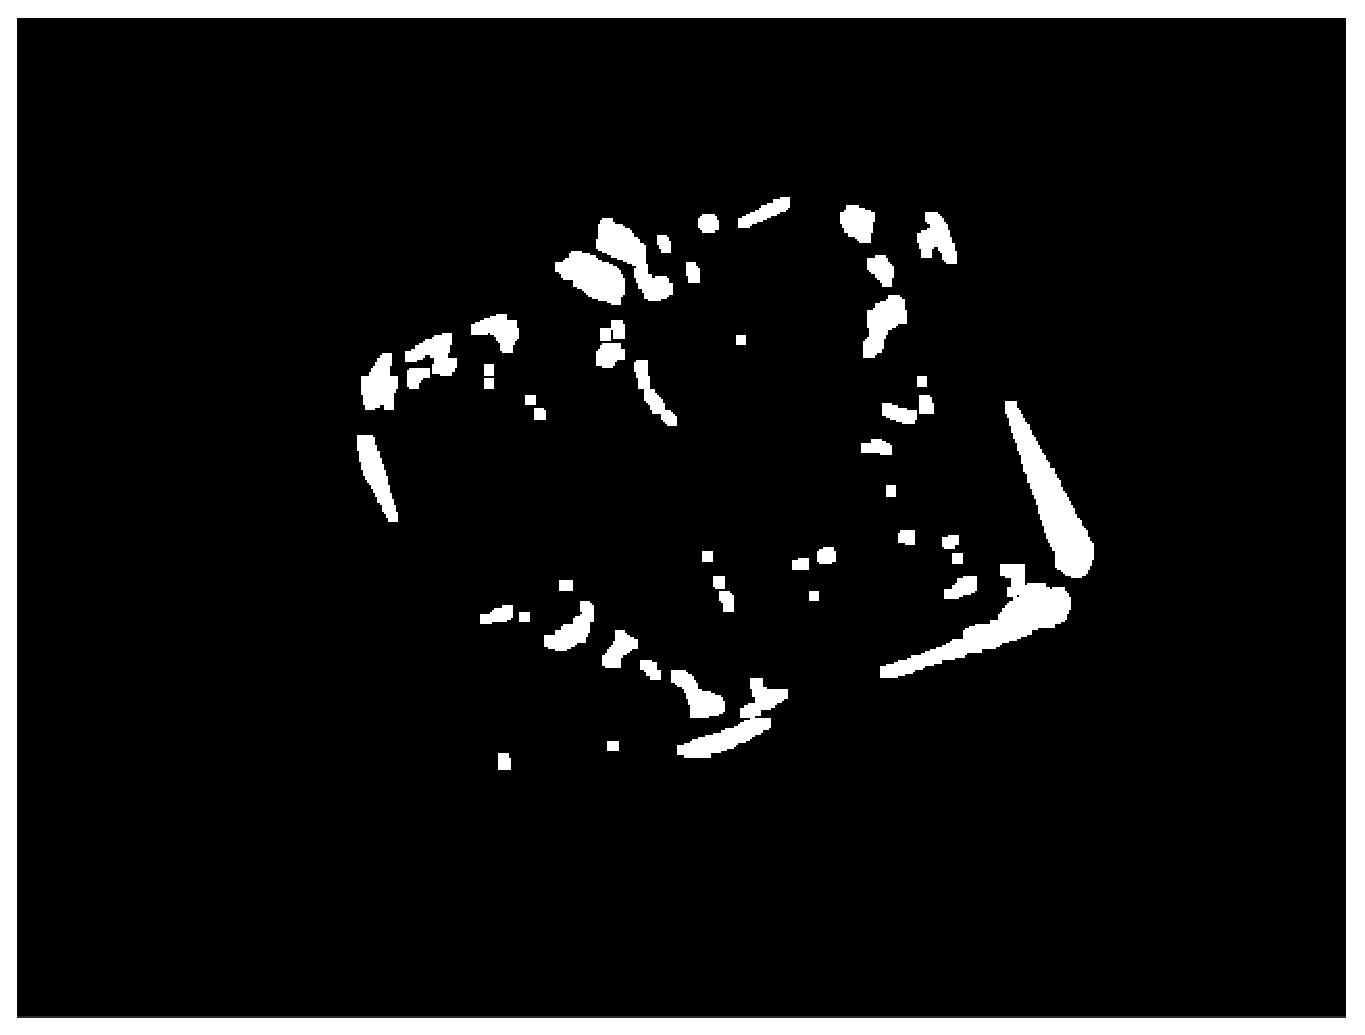
\includegraphics[width=0.27\textwidth]{../../figs/preprocess/dilate} \label{fig:deteccion_movimietno-dilate}}
    \subfloat[][\small{BR}]{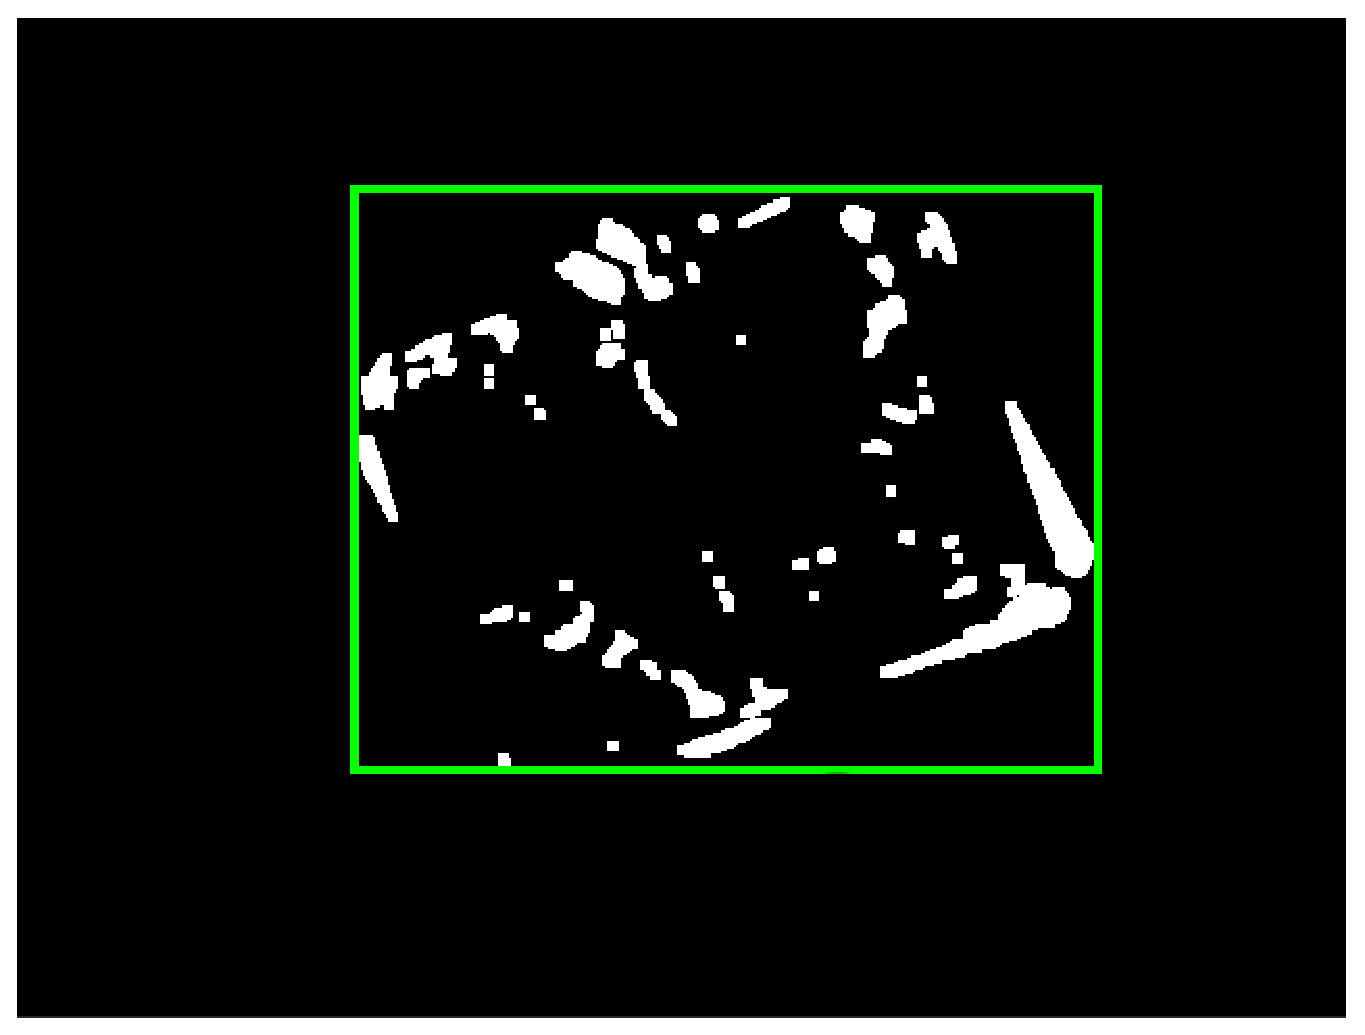
\includegraphics[width=0.27\textwidth]{../../figs/preprocess/boundingrect} \label{fig:deteccion_movimietno-boundingrect}}
    \caption[\small{Detección de movimiento}]{\small{Resultado de los procesos aplicados para la detección de movimiento.}}
    \label{fig:deteccion_movimiento}               %% Etiqueta para la figura entera
  \end{figure}
\end{frame}

% ver si pongo esto o no!!??
% \begin{frame}{Área de BR}
%  Si el area de BR > 10000 píxeles se continua con el proceso, sino se deriva
% \end{frame}

\subsection{Extracción de Características}
  %ver el tema de noctaves, noctaveLayers y hessianThreshold -> como no lo pongo me parece que lo debería mencionar
  \begin{frame}{Detección de puntos claves y descriptor}
      \begin{block}{\textbf{SURF} (Detector rápido de características robustas)}
	\begin{itemize}
	      \item Detector y descriptor de puntos claves.
		  \note[item]{blob detection refers to mathematical methods that are aimed at detecting regions in a digital image that differ in properties, such as brightness or color, compared to areas surrounding those regions. Informally, a blob is a region of a digital image in which some properties are constant or vary within a prescribed range of values; all the points in a blob can be considered in some sense to be similar to each other.}
	      \item Basado en \textbf{SIFT} (Transformación de características invariante a la escala).
	      \item Gran velocidad de cálculo (más rápido que SIFT) con tolerable pérdida de robustez. %(No está basados en kernels de punto flotante)
	\end{itemize}
      \end{block}
  \end{frame}
 %
 \begin{frame}{El problema de cambio de escala en correspondencias de puntos}
    \begin{itemize}
      \item Los objetos fotografiados a diferentes distancias, aparecen de diferente tamaños.
	  \note[item]{Si tomamos varias fotografias de un objeto a diferentes distancias, el objeto aparecerá de diferente tamaño}
      \item Buscar correspondencias utilizando un número fijo de píxeles vecinos $\rightarrow$ las intensidades no coincidirán.
	  \note[item]{Luego, si se tratan de buscar correspondencias entre las imágenes del objeto usando un tamaño FIJO de píxeles vecinos, la intensidad no coincidirá debido al cambio de escala presenten en las mismas y por lo tanto el reconocimiento fallará.}
      \item Definir un área vecina al punto clave con la misma información visual.
	  \note[item]{La escala define un área vecina con la misma información visual.
		  La motivación de generar una representación espacio escala se origina en que los objetos reales están compuestos por diferentes estructuras a diferentes escalas. Dependiendo de la escala de observación aparecen de diferentes tamaños. Por ejemplo el concepto de un árbol es apropiado a la escala de metros, pero el concepto de hojas o moléculas son apropiados para escalas más finas.}
    \end{itemize}
	    \note[item]{Si la escala del filtros gaussiano es muy pequeña, el resultado incluye muchos puntos redundantes de detalles innecesarios}
		\note[item]{Contrariamente, si la escala es muy grande, los puntos de regiones con soporte pequeño tienen a desaparecer con el borroneado}
		\note[item]{Para solucionar los problemas existentes en el filtrado gaussiano con escalas fijas, se han propuesto procedimientos espacio-escala basados en la representación de la curvatura discreta multi escalar}
 \end{frame}

 \begin{frame}
      \begin{block}{SURF}
	\begin{itemize}
	      \item Invariante a escala: asigna un factor de escala a cada punto clave.
		\note[item]{mediante el calculo del laplaciano usando filtros gaussianos a diferentes escalas.}
		\note[item]{La localización de los puntos se realiza mediante una interpolación con una función cuadrática. Esto se hace porque en filtros de tamaños grandes, el muestreo es grande y esto en la imágen representan a largas distancias respecto de la imagen base por asi decirlo}
	      \item Invariante a rotación: asigna una orientación a cada punto clave.
		  \note[item]{Asigna una orientación a cada punto detectado}
	      \item Determinante de la matriz hessiana para la determinación de la localización y escala de los puntos $\rightarrow$ umbral
		  \note[item]{puntos que superan un umbral son extraídos}
	      \item Vector descriptor $N$ dimensional (64 elementos) para cada punto clave.
		  \note[item]{La región es dependiente de la escala en que fue detectado el punto!!!}
		  \note[item]{$\rightarrow$ posibles de comparar con una métrica de distancia}
		  \note[item]{Región centrada en el punto clave (de tamaño dependiente de la escala) y en orientada de acuerdo a la orientación detectada anteriormente sobre la que se realizan diversas operaciones}
	      \item Cuanto más similares sean 2 puntos característicos más cercanos serán sus descriptores.
		  \note[item]{describe cómo las intensidades de los píxeles se distribuyen dentro de una vecindad, que es dependiente de la escala de cada punto de interés detectado por el hessiano}
		  \note[item] {Cuando el determinante del hessiano es un máximo local (previa eliminación de mínimos mediante un umbral), se determina un punto clave. El uso del hessiano es alentado por su velocidad de cálculo y precisión.
		  \begin{equation*}
		    H(x,y)=\begin{bmatrix}\frac{\partial^{2}I}{\partial x^{2}} & \frac{\partial^{2}I}{\partial x\partial y}\\
		    & \\
		    \frac{\partial^{2}I}{\partial y\partial x} & \frac{\partial^{2}I}{\partial y^{2}}
		    \end{bmatrix};\; \textrm{con}\; \frac{\partial^{2}I}{\partial x\partial y}=\frac{\partial^{2}I}{\partial y\partial x}.
		    \label{eq:HessianMatrix}
		  \end{equation*}
		  Sea $\mathbf{p}=(x,y)$ un punto en la imagen $\mathit{I}$
		  la matriz hessiana en $\mathbf{p}$ en la escala $\sigma$ viene definida como:
		  \begin{equation*}
		    \mathcal{H}(\mathbf{p},\sigma)=\left[\begin{array}{cc}
		    \mathit{L_{xx}(\mathbf{p},}\sigma)\hphantom{} & \mathit{L_{xy}(\mathbf{p},}\sigma)\\
		    \mathit{L_{xy}(\mathbf{p},}\sigma)\hphantom{} & \mathit{L_{yy}(\mathbf{p},}\sigma)
		    \end{array}\right],
		  \end{equation*}
		  $\mathit{L_{xx}(\mathbf{p},}\sigma)$ es la convolución de la derivada segunda de una gaussiana $\frac{\partial^{2}}{\partial x^{2}}\mathit{g}(\sigma)$ con la imagen $\mathit{I}$ en el punto $\mathbf{p}$
		  }
		  \note[item]{$\mathit{L_{xx}(\mathbf{p},}\sigma)$ es la convolución de la derivada segunda de una gaussiana $\frac{\partial^{2}}{\partial x^{2}}\mathit{g}(\sigma)$ con la imagen $\mathit{I}$ en el punto $\mathbf{p}$}
		  \note[item]{$\mathit{L_{xy}(\mathbf{p},}\sigma)$ es la convolución de la derivada segunda de una gaussiana $\frac{\partial^{2}}{\partial x \partial y}\mathit{g}(\sigma)$ con la imagen $\mathit{I}$ en el punto $\mathbf{p}$}
		  \note[item]{$\mathit{L_{yy}(\mathbf{p},}\sigma)$ es la convolución de la derivada segunda de una gaussiana $\frac{\partial^{2}}{\partial y^{2}}\mathit{g}(\sigma)$ con la imagen $\mathit{I}$ en el punto $\mathbf{p}$.}
	\end{itemize}
      \end{block}
  \end{frame}
% \begin{frame}{SURF}
% % 	  \begin{figure}[tbhp]
% % 	    \centering
% % 		  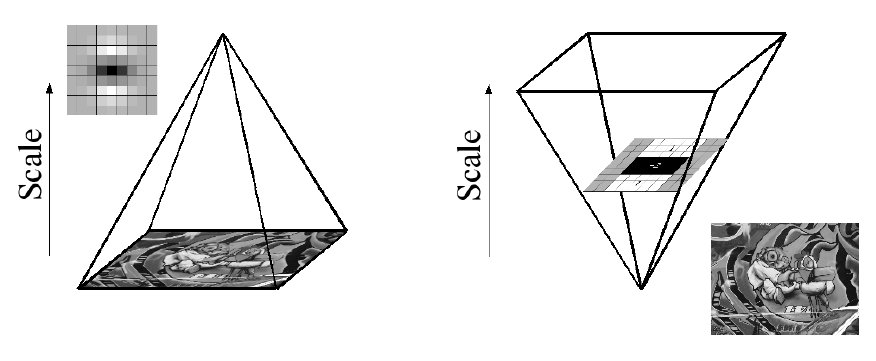
\includegraphics[scale=0.41]{../../figs/pyramidfilters}
% % 	      \caption[Pirámide de escala de imágenes para SIFT y SURF]{Pirámide de escala de imágenes para el método SIFT (izquierda) y el método SURF (derecha).}
% % 	    \label{fig:pyramidfilters}          %% Etiqueta para la figura entera
% % 	  \end{figure}
% 
% 	  %aclarar el tema de los box filters y de las imagenes integrales
% 	       
% 	       \begin{figure}[tbhp]
% 		  \centering
% 		  %%----primera subfigura----
% 		  \subfloat[]{
% 			\label{fig:gaussiankernelsdiscreted_y}         %% Etiqueta para la primera subfigura
% 			\includegraphics[scale=0.3]{../../../img_ent2/gaussiankernelsdiscrete_y}}
% 			\hspace{0.1\linewidth}
% 		  %%----segunda subfigura----
% 		  \subfloat[]{
% 			\label{fig:gaussiankernelsaprox_y}         %% Etiqueta para la segunda subfigura
% 			\includegraphics[scale=0.3]{../../../img_ent2/gaussiankernelsaprox_y}}
% 			\hspace{0.1\linewidth}
% 		  %%----tercera subfigura----
% 		  \subfloat[]{
% 			\label{fig:gaussiankernelsdiscreted_xy}         %% Etiqueta para la segunda subfigura
% 			\includegraphics[scale=0.3]{../../../img_ent2/gaussiankernelsdiscrete_xy}}
% 			\hspace{0.1\linewidth}
% 		  %%----cuarta subfigura----
% 		  \subfloat[]{
% 			\label{fig:gaussiankernelsaprox_xy}         %% Etiqueta para la segunda subfigura
% 			\includegraphics[scale=0.3]{../../../img_ent2/gaussiankernelsaprox_xy}}
% 			\hspace{0.1\linewidth}
% 		\caption[\scriptsize{Derivadas parciales gaussianas discretas y aproximadas}]{\scriptsize{Derivadas parciales gaussianas de segundo orden discretas y sus homólogas aproximadas (también referenciadas como filtros tipo caja). Las regiones grises de la imagen son iguales a cero.}}%% Etiqueta para la figura entera
% 		  \label{fig:gaussiankernels}
%       \end{figure}
%       SURF utiliza filtros aproximados (Box filters) \note[item]{combinado con el uso de imágenes integrales, se calcula más rápidamente}
% 	  \note[item]{Así el determinante de la matriz hessiana (aproximado) usado por SURF queda definido como:}
% 	  \begin{equation*}
% 	    \label{eq:det_happrox}
% 	    \det(\mathcal{H}_{approximado})=D_{xx}D_{yy}-(wD_{xy})^{2} 
% 	  \end{equation*}
% 	  con $w=0.9$ y donde $\mathit{D}_{xx}$, $\mathit{D}_{yy}$ y $\mathit{D}_{xy}$ son las derivadas parciales gaussianas de segundo orden aproximadas.
% 	  \note[item]{ La ponderación relativa $w$ de la respuesta del filtro es usada para balancear la expresión del determinante hessiano. Si bien el mismo varía para diferentes escalas, en la práctica se puede establecer este factor como constante con $w=0.9$, ya que el mismo no tiene un impacto significante en los resultados}
% \end{frame}

% \begin{frame}{SURF}
%   \begin{block}{Puntos claves}
% 	\begin{itemize}
% 	    \item Asigna un factor de escala a cada punto clave detectado.
% 	    \item La escala define un área vecina con la misma información visual
% 	    \item Asigna una orientación a cada punto detectado 
% 	\end{itemize}
%   \end{block}
% 
%   \begin{block}{Descriptores}
%       \begin{itemize}
% 	\item Región centrada en el punto clave (de tamaño dependiente de la escala) sobre la que se realizan diversas operaciones
% 	\item Se crea un vector N dimensional (64 elementos) por cada punto clave $\rightarrow$ posibles de comparar con una métrica de distancia,
% 	\item Cuanto más similares sean 2 puntos característicos más cercanos serán sus descriptores.  
%       \end{itemize}
%   \end{block}
% \end{frame}

% \begin{frame}{El problema de cambio de escala en correspondencias de puntos}
%  \begin{itemize}
%   \item Tener un factor de escala asociado con cada punto detectado.
%   \item Calculo del laplaciano de un punto en una imagen usando filtros gaussianos a diferentes escalas.
%     \note[item]{Si la escala del filtros gaussiano es muy pequeña, el resultado incluye muchos puntos redundantes de detalles innecesarios}
%     \note[item]{Contrariamente, si la escala es muy grande, los puntos de regiones con soporte pequeño tienen a desaparecer con el borroneado}
%     \note[item]{Para solucionar los problemas existentes en el filtrado gaussiano con escalas fijas, se han propuesto procedimientos espacio-escala basados en la representación de la curvatura discreta multi escalar}
%     \note[item]{El esquema está basado en el criterio de estabilidad que establece que la presencia de una esquina debe ocurrir como un máximo de curvatura observable en la mayoría de las escalas} %\cite{springerlink:10.1023/A:1008045108935}
%   \item Mediante las respuestas para diferentes escalas, se obtiene una curva que alcanza un valor máximo en algún valor de $\sigma$ (varianza de la función gaussiana) 	  \note[item]{$\sigma$ define implícitamente la escala en que la derivada es evaluada.}
%   \item Si se extrae este valor para dos imágenes del mismo objeto (tomadas a diferentes esclas), la relación que existe entre los $\sigma$ máximos se corresponderán en relación con las escalas en que fueron tomadas cada una de las fotografías.
%     \note[item]{Esta observación es el núcleo del proceso de extracción de características invariantes a la escala}
%  \end{itemize}
% \end{frame}

% \begin{frame}{Invarianza a escala}  
% 	\begin{center}
% 	    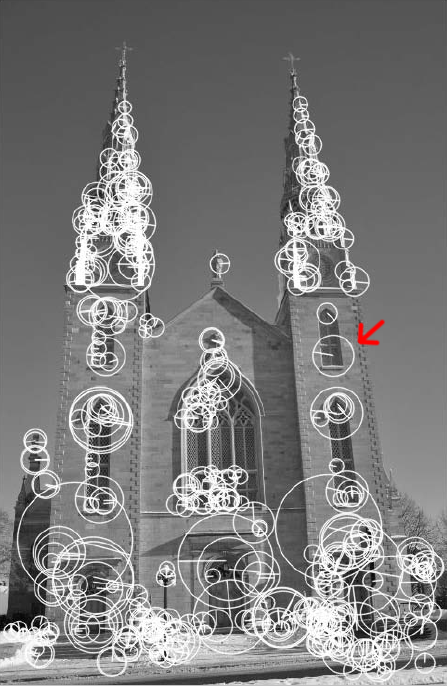
\includegraphics[scale=0.3]{./img1/surfinchurch1} \qquad
% 	    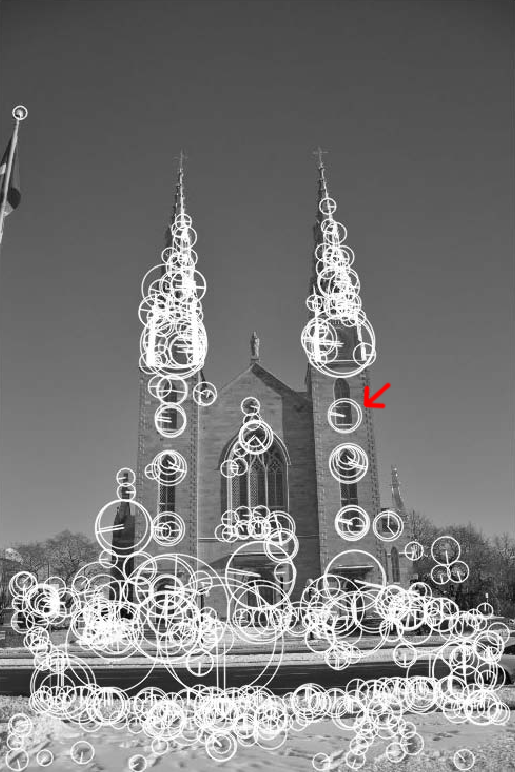
\includegraphics[scale=0.267]{./img1/surfinchurch2}
% 	\end{center}
% \end{frame}

%%%%%%%%%%%%%%%%%%%%%%%%%%%%%%%%%%%%%%%%%%%%%%%%%%%%%%%%%
\subsection{Correspondencia de puntos entre imágenes}
\begin{frame}{Búsqueda de correspondencias}
    \note[item]{calcular un valor que represente el grado de similitud de dos imágenes}
    \begin{block}{Grado de similitud}
    Grado de similitud entre vectores mediante distancia euclídea.
      \begin{itemize}
	\item NNS (Búsqueda del vecino más cercano).
	    \note[item]{Dado un conjunto de puntos $P=\left\{ p_{1,...,}p_{n}\right\}$ en un espacio métrico $M$ y un punto de consulta $q \in M$, encontrar el punto más cercano a $q$ en $P$ de forma eficiente, donde $M$ es un espacio euclídeo d-dimensional y la distancia es medida por ejemplo mediante la distancia euclídea.
	    }
	      \note[item]{$\root{(x_2-x_1)^2+(y_2-y_1)^2}$ - La distancia entre dos puntos es igual al módulo del vector que tiene de extremos dichos puntos.}
	      \note[item]{El módulo de un vector es la longitud del segmento orientado que lo define. $P=(3,4) entonces \root{3^2+4^2})$}
	\item $K$-NN (K vecinos más cercanos).
	  \note[item]{si $K=1$ $\rightarrow$ NNS}	
	\item Búsqueda aproximada mediante $KD$-tree o multiple $KD$-tree aleatorio.
	  \note[item]{Se usan 2 o 4 árboles examinándose todas las hojas (las 64) y buscando los 2 vecinos más cercanos}
	  \note[item]{Búsqueda aproximada del vecino más cercano $\rightarrow$ mejora los tiempos de ejecución con errores de precisión aceptables.}
	  \note[item]{
	    \begin{itemize}
	    \item KD-tree: 
		  \note[item]{Los elementos guardados en el árbol KD-tree, son vectores de altas dimensiones}
		  \note[item]{Para construir el árbol, se compara el vector de entrada con el ``valor de partición'' para determinar a qué mitad del árbol pertenece dicho vector. Cada una de las dos mitades de los datos es dividida de igual manera y en forma recursiva, para lograr crear un árbol binario completamente balanceado.}
		  \begin{itemize}
		      \item Creación de una estructura de árbol para la búsqueda 
			    \note[item]{En la raíz del árbol (primer nivel), los datos son divididos en dos mitades por un hiper plano ortogonal para una dimensión elegida y con un valor de umbral.}
			    \note[item]{Generalmente, esta división se realiza con la media, en la dimensión con la mayor varianza del conjunto de datos (para SIFT y SURF es la medida que presenta el mejor rendimiento)}
		      \item Eficiente con datos de bajas dimensiones
		  \end{itemize}
	    \item Múltiples árboles KD aleatorios \note[item]{Para acelerar la búsqueda}
	    \begin{itemize}
		  \item Búsqueda eficiente con datos de altas dimensiones
		      \note[item]{Los árboles aleatorios son construidos seleccionando la dimensión de división de forma aleatoria sobre las primeras $D=5$ dimensiones en las que los datos poseen mayor varianza.}
		      \note[item]{Cuando se realiza la b\'usqueda en el árbol, una cola con prioridad es mantenida a través de todos los arboles aleatorios, por lo que la búsqueda queda ordenada mediante el incremento de la distancia a cada nodo del borde.}
		      \note[item]{El grado de aproximación, se determina mediante el examen de un número fijo de nodos hoja.}
		      \note[item]{Cuando es alcanzado este número, se termina la búsqueda y se obtienen los candidatos.}
		  \item Se obtiene resultados aproximados
		  \item La cantidad de memoria utilizada aumenta
			\note[item]{Se debe tener en cuenta que la cantidad de memoria utilizada aumenta linealmente con el número de árboles aleatorios, una característica negativa cuya importancia no resulta menor en la sobrecarga del sistema.}
	      \end{itemize}
	    \end{itemize}
	}	
    \end{itemize}
  \end{block}
\end{frame}

\begin{frame}{Búsqueda de correspondencias}
  \begin{itemize}
  \item Cálculo de la distancia euclídea entre los vectores característicos.
    \note[item]{Las correspondencias son buscadas mediante el cálculo de la distancia euclídea entre los vectores característicos asociados a los puntos claves detectados en cada una de las imágenes.}
  \item Aplicación de un umbral para determinar las potenciales correspondencias válidas.
    \note[item]{se usa una relación entre el vecino más cercano y el segundo vecino más cercano}
%   \item Umbral global que se compare con la distancia a la característica más cercana no funciona correctamente
%   \note[item]{Usar un valor de umbral global que se compare con la distancia a la característica más cercana no funciona correctamente}
%   \item Se propone comparar la distancia del vecino más cercano ($d_1$) respecto del segundo vecino más cercano ($d_2$).
      \note[item]{$A$ y $B$ dos imágenes sobre las cuales se quieren buscar correspondencias}
      \note[item]{Consideremos $a_i$ con $i=0\ldots n$ un punto del conjunto de puntos claves detectados en $A$}
      \note[item]{$n$ el total de puntos claves detectados en $A$}
      \note[item]{$av_i$ el vector característico asociado al punto $a_i$}
      \note[item]{Para cada $a_i$, se seleccionan los dos mejores puntos claves candidatos $p_1 \in b_i$ y $p_2 \in b_i$ cuyos vectores de características asociados a cada uno representan las distancias euclídeas mínimas $d_1$ y $d_2$ respectivamente respecto a $av_i$}
%   \item Si $\frac{d_{1}}{d_{2}}>0.8$ la coincidencia es rechazada.
      \note[item]{con 0.6 es un poco más rápido pero menos estable}
      \note[item]{se puede interpretar como: si las dos coincidencias más cercanas no difieren por mucho, es un problema porque no sabemos cual de las dos es la correcta}
      \note[item]{Las coincidencias buenas necesitan tener el vecino más cercano, significativamente más cerca que las correspondencia mala}
      \note[item]{Aplicar un umbral global no funciona correctamente ya que algunos descriptores son más descriminativos que otros. Una medida más efectiva es usar la que usamos aquí: Muchas características de la imagen no tiene la correspondencia correcta en la imagen de entrenamiento ya que surgen de objetos del fondo por ejemplo. La idea es eliminar las características que no tienen una buena correspondencia.}
      \note[item]{El valor de $\varepsilon=0.8$ fue seleccionado de acuerdo al estudio llevado a cabo por Lowe que afirma que se alcanzan a eliminar un 90\% de falsas coincidencias mientras se descartan sólo un 5\% de buenas coincidencias, resultando en el valor más apropiado. Valores de $\varepsilon=0.6$ a $0.9$ también son apropiados.}
  \item Reducción de correspondencias espurias.
      \note[item]{Eliminar coincidencias espurias realza la habilidad de buscar la homografía correcta mediante la}
  \end{itemize}
\end{frame}
% \begin{frame}{Comparación}
% Encontrar correspondencias entre la imagen patrón y la imagen del flujo de video.
% 	\begin{itemize}
% 		\item Correspondencia de características entre imágenes
% 		\item Patrón buscado presente en imagen capturada? $\rightarrow$ Comparación de vectores característicos de imagen Patrón y Frame del flujo de video.
% 	\end{itemize}
% \end{frame}
% 
% \begin{frame}{Herramientas}
% 	\begin{itemize}	
% 		\item Métrica de distancia (euclídea, manhattan, etc.)
% 		\item Vectores de grandes dimensiones (NNS por fuerza bruta - lento).
% 		\item Variante para reducir tiempos: Multiples árboles aleatorios KD-tree.
% 		\item Retorna los mejores candidatos (aproximados)
% 	\end{itemize}
% \end{frame}
%%%%%%%%%%%%%%%%%%%%%%%%%%%%%%%%%%%%%%%%%%%%%%%%%%%%%%%%%

\subsection{Transformación y RA}
\begin{frame}{Transformación proyectiva - Homografía}
\note[item]{Marcelo: Transformación proyectiva !ojo! no es lo mismo imagen que el objeto y los puntos del objeto son los que buscamos.
}
 \begin{itemize}
  \note[item]{cvFindHomografphy: Se busca la transformación perspectiva entre dos planos}
  \item Relación proyectiva entre dos imágenes de una misma escena tomadas desde diferentes puntos de vista.
      \note[item]{Al tomar dos imágenes de una misma escena desde diferentes puntos de vista, existe una importante relación proyectiva entre éstas y la escena.}
      \note[item]{Una transformación proyectiva (también conocida con los términos equivalentes: colineación u homografía) es un mapeo invertible $h$ de $\mathbb{P}^2$ a sí mismo, de tal manera que tres puntos $x_1, x_2, x_3$ están sobre la misma línea si y solo si $h(x_1), h(x_2), h(x_3)$ también lo están. }
      %     \begin{block}{Transformación proyectiva}
      %       Un mapeo $h$: $\mathbb{P}^2 \rightarrow \mathbb{P}^2$ es una transformación proyectiva si y solo si existe una matriz de $3 \times 3$ ($\textit{H}$) tal que para cada punto en $\mathbb{P}^2$ representado por un vector $\mathbf{x}$ se cumple que $h(\mathbf{x})=\textit{H}(\mathbf{x})$. 
      %     \end{block}
      
  \item La relación entre las dos imágenes es una homografía si se cumple la ecuación $\textbf{x'}=H\textbf{x}$: 
      \note[item]{Si consideramos el conjunto de puntos $(x_i,y_i,z_i)$ perteneciente a una primer imagen y sabemos que mapean a un conjunto de puntos $(x'_i, y'_i, z'_i)$ en la segunda imagen (ambos en coordenadas homogéneas), la relación entre las dos imágenes es una homografía si se cumple la ecuación} %\eqref{eq:eq_cumple_homografia}.
      \begin{equation*}
	\begin{bmatrix}
	x'_i\\
	y'_i\\
	z'_i
	\end{bmatrix}=\textit{H}
	\begin{bmatrix}
	x_i\\
	y_i \\
	z_i
	\end{bmatrix}\Longrightarrow
      \begin{bmatrix}
	x'_i\\
	y'_i\\
	z'_i
	\end{bmatrix}=
	\begin{bmatrix}
	h_{11} & h_{12} & h_{13}\\
	h_{21} & h_{22} & h_{23}\\
	h_{31} & h_{32} & h_{33}\\
	\end{bmatrix}
      \begin{bmatrix}
	x_i\\
	y_i \\
	z_i
	\end{bmatrix}.
	\label{eq:eq_cumple_homografia}
      \end{equation*}
      \item Los puntos en una vista pueden ser convertidos a la segunda vista mediante $H$.
	\note[item]{Una vez que se a logrado obtener $\textit{H}$, todos los puntos en una vista pueden ser convertidos a la segunda vista usando esta relación.}
	\note[item]{Dos Fotografías de diferentes puntos de vista (imagen patrón y frame de flujo de video).}
	\note[item]{En qué lugar un punto en una fotografía se encuentra en la otra $\rightarrow$ Matriz homográfica.}
	\note[item]{Busca la transformación perspectiva entre dos planos. $x'=Hx$}
  \end{itemize}
\end{frame}

\begin{frame}{Estimación de $H$}
\note[item]{La homografía transformación proyectiva u homografía, es la proyección perspectiva entre dos imágenes y es derivada de las posiciones de los puntos claves en la imagen patrón y los puntos coincidentes detectados en la imagen objetivo.}
  \begin{itemize}
  \item Se pueden tener pares de correspondencias que no son válidos o tener más de 4 pares de correspondencias necesarios para calcular $H$.
      \note[item]{Un punto $2D$ $(x,y)$ en una imagen es representado por un vector $3D$ $\textbf{x}=(x_1,x_2,x_3)$ donde $x=\frac{x_1/x_3}$ y $y=\frac{x_2/x_3}$. Esto es llamado representación homogénea de un punto y se encuentra sobre el plano proyectivo $P^2$. Se debe notar que $H$ puede cambiar multiplicandose por una constante arbitraria no cero sin alterar la transformación proyectiva. Es decir que $H$ es considerada una matriz homogénea y tiene solo 8 grados de libertad a persa de contener 9 elementos. Es decir que hay 8 incógnitas que se tienen que resolver.}
      \note[item]{La transformación proyectiva u homografía es una transformación lineal no singular de coordenadas homogéneas: transformación lineal que tiene inversa}
      \note[item]{¿¿Cuáles pares coinciden con la estimación?}
      \note[item]{Cuatro pares son necesarios para estimar la homografía}
      \note[item]{en cuyo caso la matriz $\textit{H}$ puede resultar incorrecta}
  \item Se procede mediante una estimación de la homografía.
      \note[item]{Determinar la ``mejor'' transformación a partir de los datos, lo cual se convierte en la búsqueda de la transformación $\textit{H}$ que minimice una función de costo.}
  \item RANSAC (\textit{random sample consensus}) puede hallar la mejor solución aproximada minimizando el error y depurando coincidencias válidas y espurias iterativamente.
      \note[item]{Además usa más de cuatro correspondencias lo que logra una mejor estimación. Minimiza el error de reproyección creo que 5 píxeles de error?}
      \note[item]{No se utiliza LMEDS porque necesita tener certeza que hay 50\% de valores exactos}
      \note[item]{Las correspondencias deben ser lo suficientemente buenas.}
      \note[item]{Aplicación de la Matriz homográfica a la imagen a sobre imponer sobre el objeto detectado (RA)}
  \end{itemize}
\end{frame}

% \begin{frame}{Homografía}  
%   \begin{figure}[tbhp]
%     \centering
% 	  \includegraphics[scale=0.5]{../../figs/transfperspectiva}
%       \caption[Esquema de transformación perspectiva]{Esquema de transformación perspectiva utilizando la homografía $H$.}
%     \label{fig:transf_pespectiva}
%   \end{figure}
% \end{frame}

% \begin{frame}{Homografía - Detección}
%   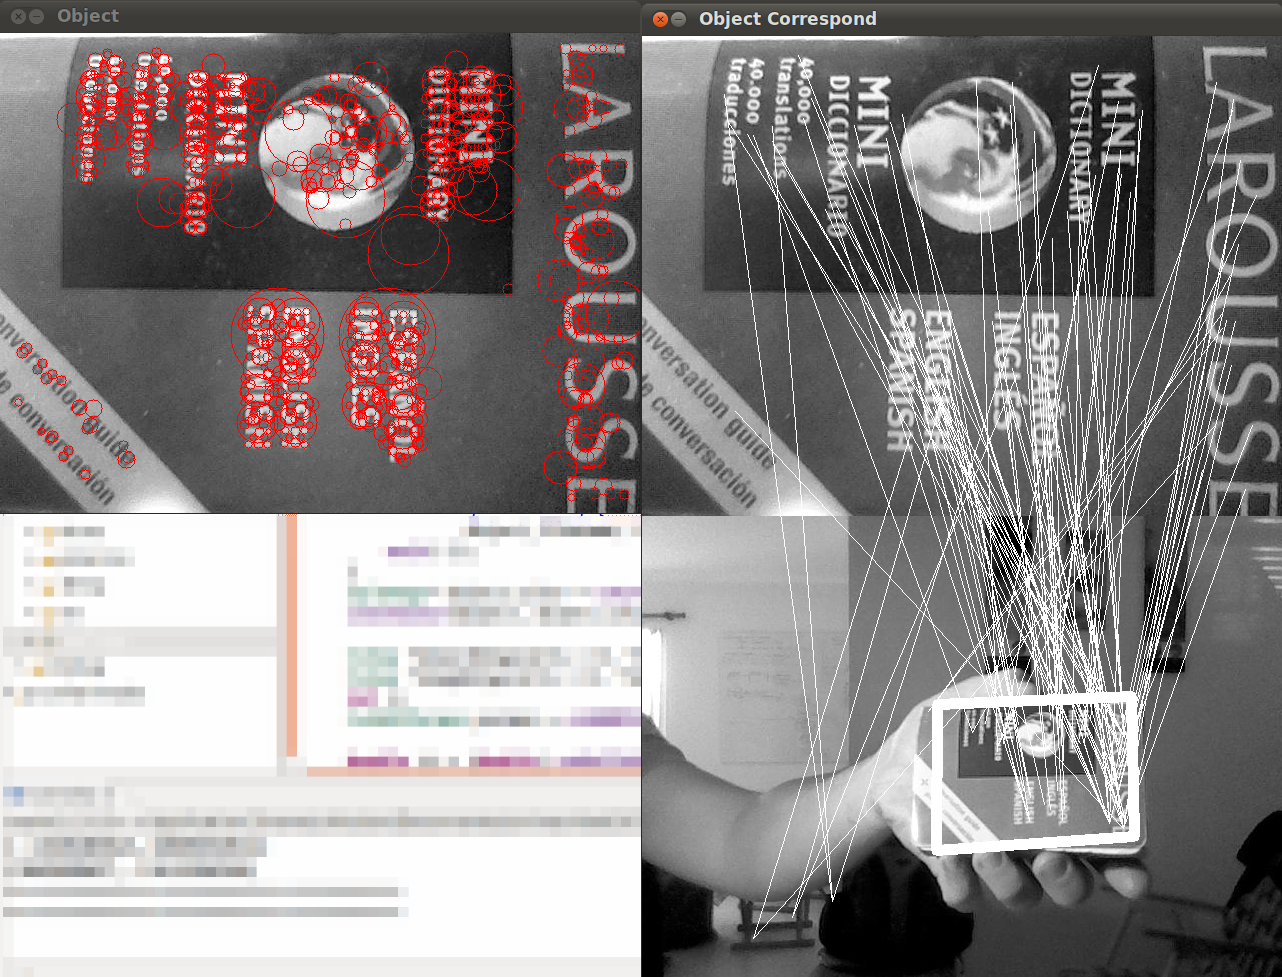
\includegraphics[scale=0.2]{./img1/correspo1}
% \end{frame}

\begin{frame}{Homografía - Detección}
  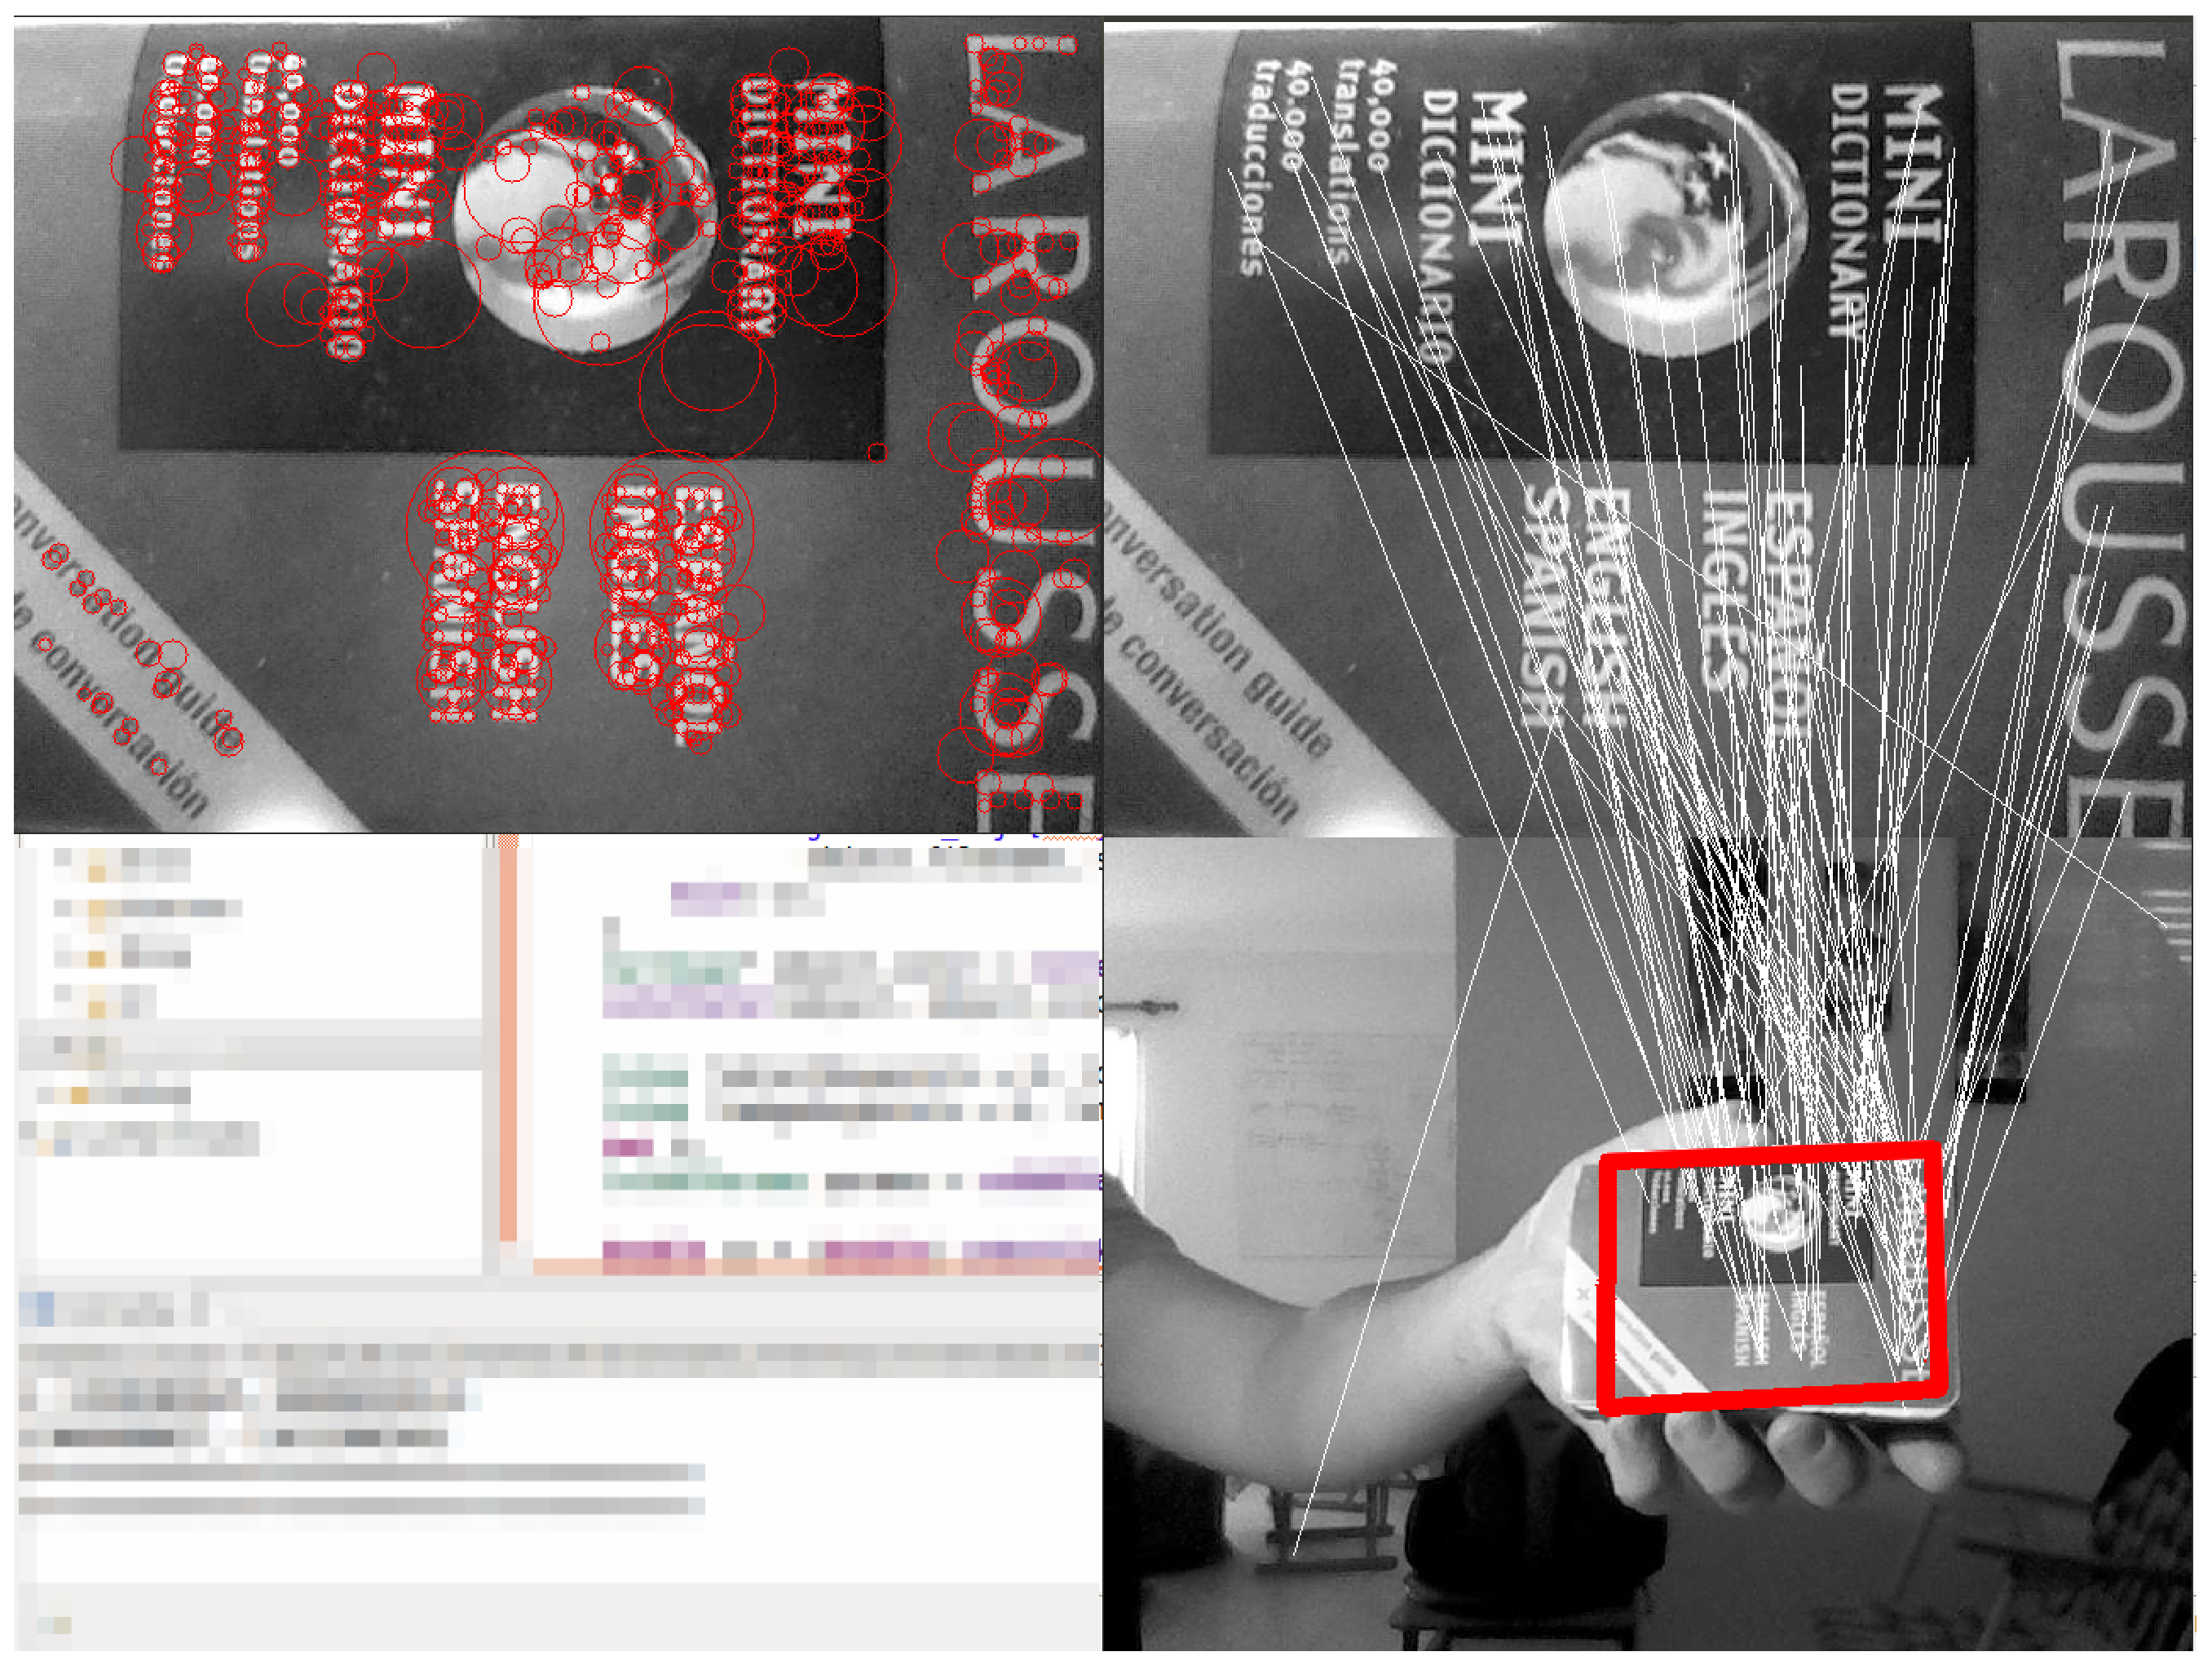
\includegraphics[scale=0.2]{./img1/correspo2_color}
    \note[item]{Explicar lo que es el recuadro rojo.}
    \note[item]{Marcelo: explicar que es lo que se vé en la imagen}
    \note[item]{Marcelo: Decir que son los círculos rojos}
\end{frame}

\begin{frame}{Homografía - Detección fallida}
  \note[item]{Explicar lo que es el recuadro rojo.}
  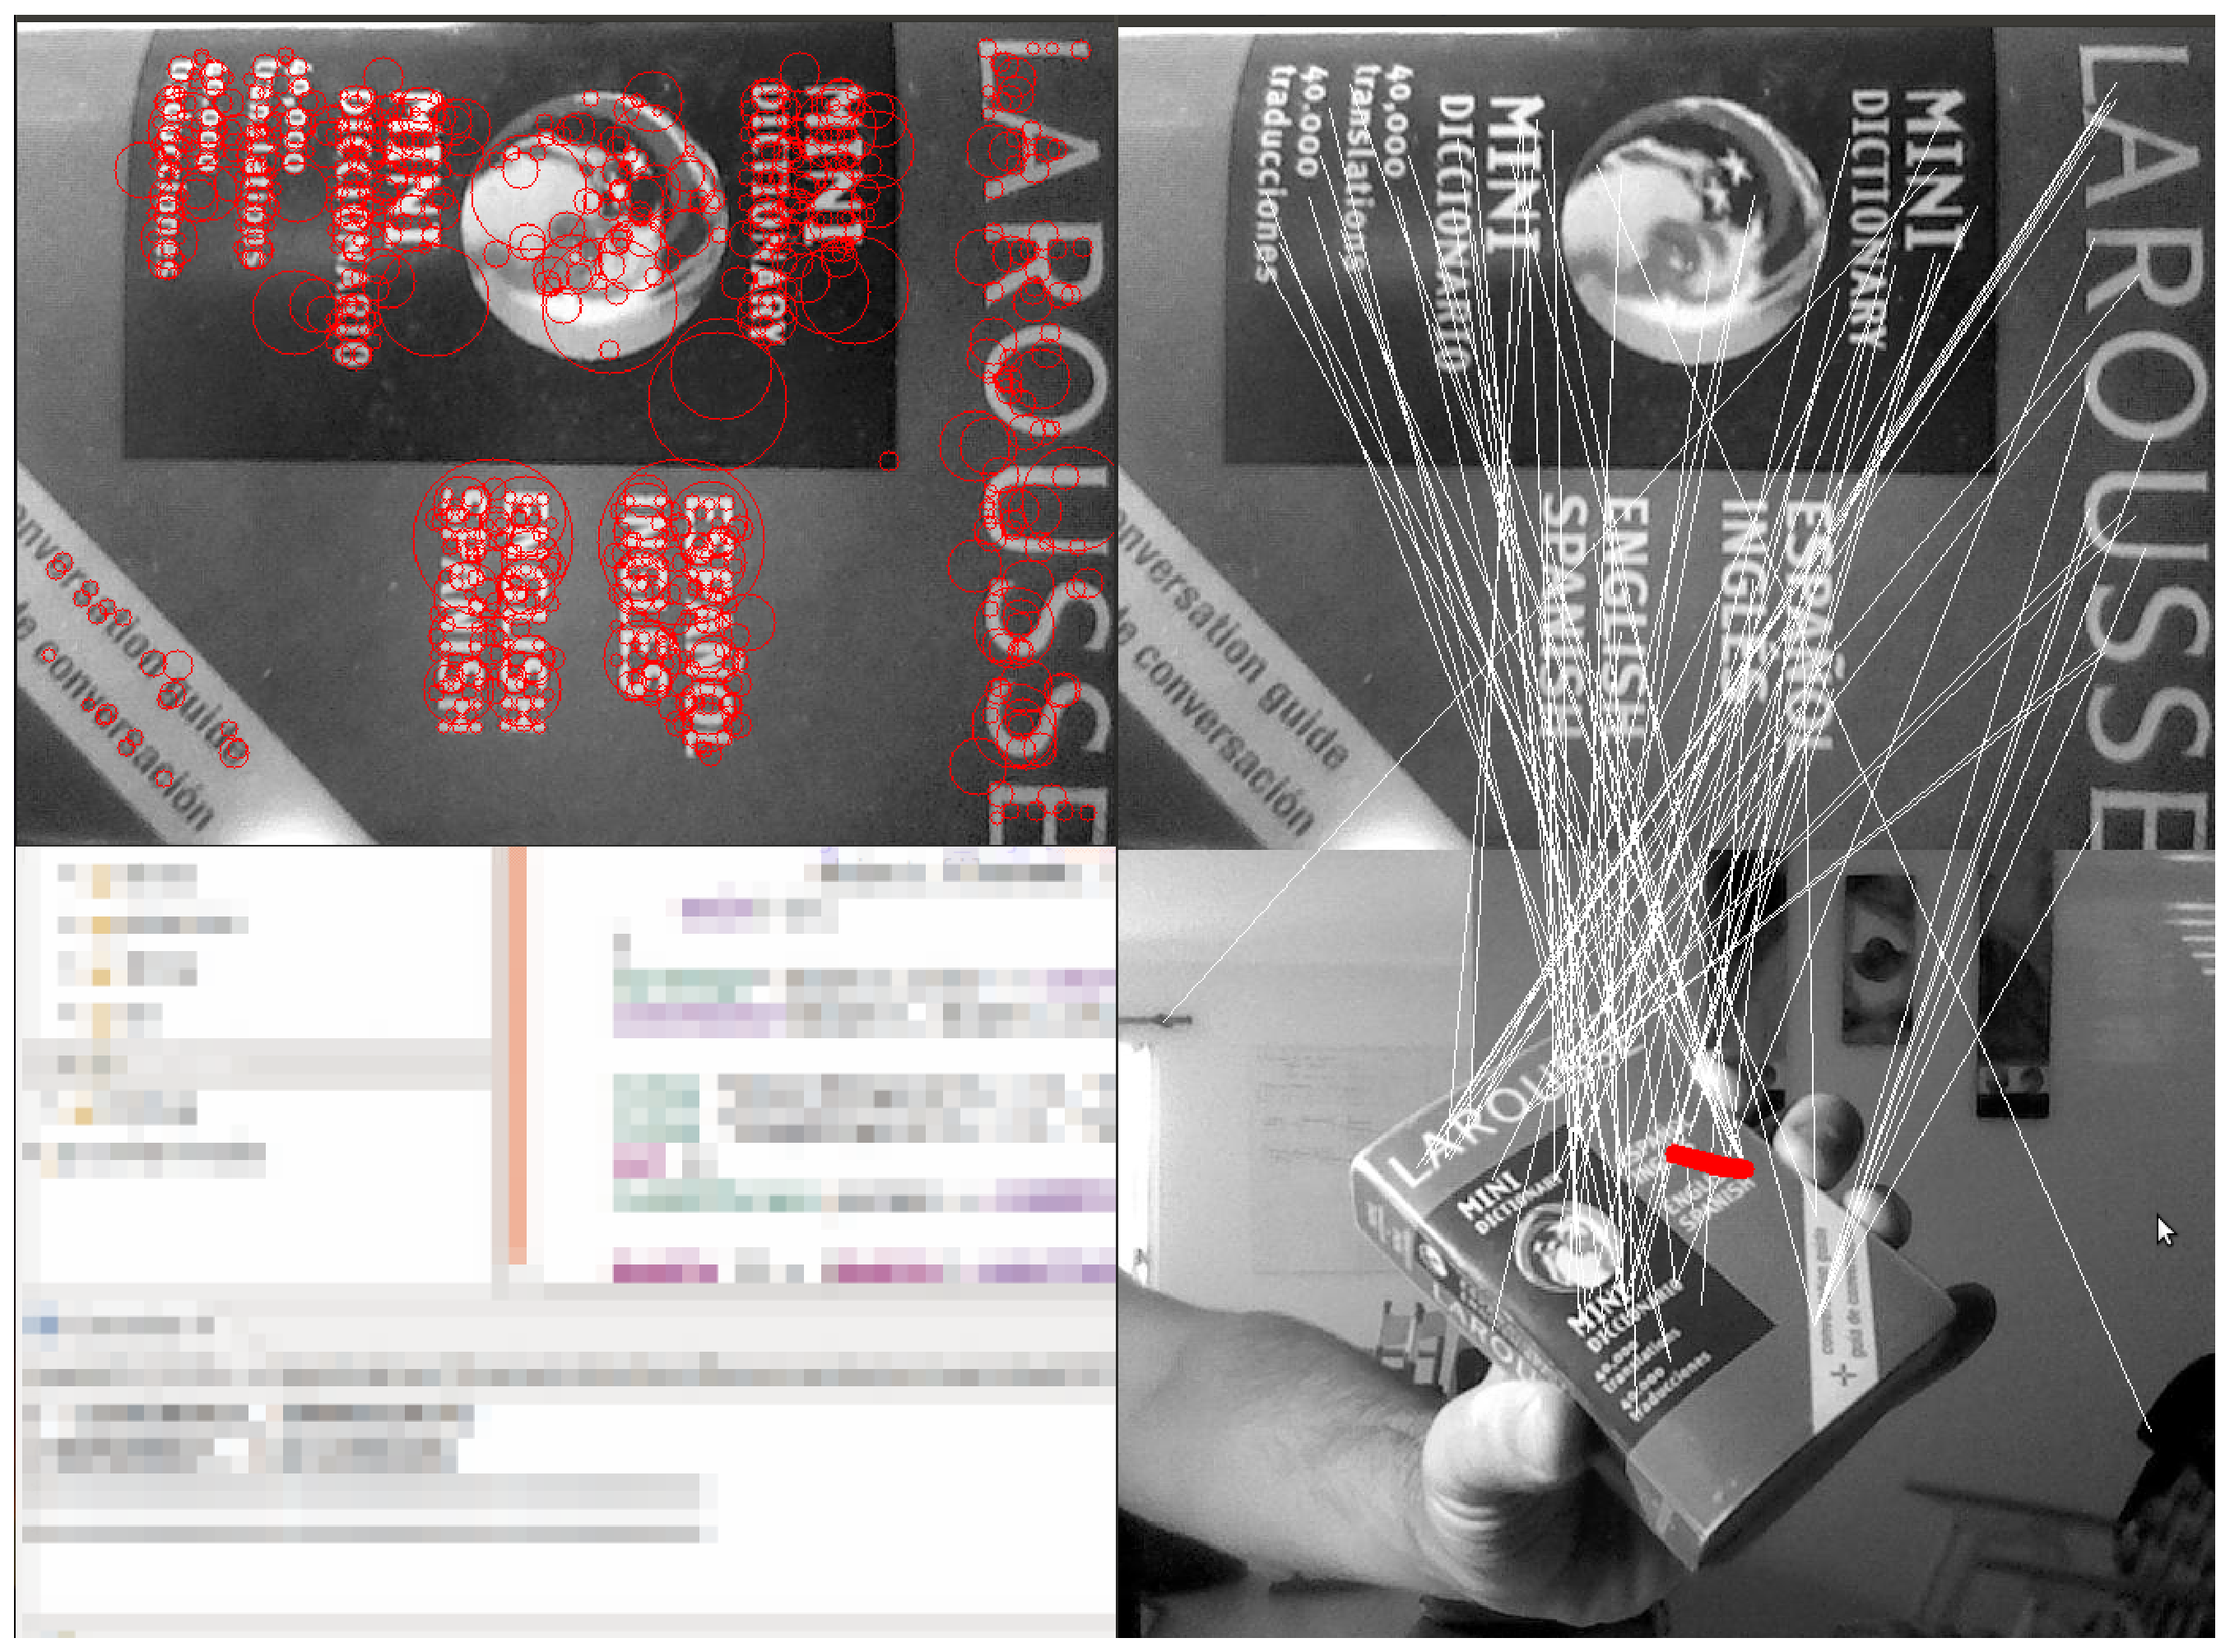
\includegraphics[scale=0.2]{./img1/correspo3_color}
\end{frame}

%%%%%%%%%%%%%%%%%%%%%%%%%%%%%%%%%%%%%%%%%%%%%%%%%%%%%%%%%
\subsection*{Validaciones}
\begin{frame}{Validación de transformaciones con $H$}
Rechazar transformación fallida
  \note[item]{ con la homografía cuando presenta una morfología inválida.}
  \begin{itemize}
      \item Comprobar convexidad. \note[item]{Se verifica convexidad del polígono generado por la transformación}
      \item Distancia entre vértices: \note[item]{(Si se satisface la condición se descarta la transformación).}
	\note[item]{Se comprueba que las esquinas opuestas en x e y no estén a menos de 20 píxeles que son las formas raras que se presentaban}
	\note[item]{
	  \begin{itemize}
	    \item $x$ y $y$ coordenadas del píxel en la imagen para el eje de las abscisas y ordenadas respectivamente
	    \item $\alpha(x,y)$, $\beta(x,y)$, $\gamma(x,y)$ y $\lambda(x,y)$ son las coordenadas de los vértices del polígono resultante de la transformación homográfica, con $\alpha$ opuesto a $\gamma$ y $\beta$ opuesto a $\lambda$,
	    \item $\Delta X=20$ y $\Delta Y=20$ es la cantidad de píxeles a comprobar entre vértices opuestos en el eje de las abscisas y ordenadas respectivamente,
	  \end{itemize}
	}
  \end{itemize}
  \small{\begin{equation*}
	  (| \alpha_x - \gamma_x| < \Delta X) \;\;\vee \;\;(| \beta_x - \lambda_x | < \Delta X) \;\;\vee \;\;(| \alpha_y - \gamma_y | < \Delta Y) \;\;\vee \;\;(|\beta_y - \lambda_y |< \Delta Y)
	  \label{eq:expresion_validacion_vertices}
	\end{equation*}}
  \begin{figure}[tbhp]
	      \centering
	      %%----primera subfigura----
	      \subfloat[\scriptsize{Polígono cóncavo}][\scriptsize{Polígono cóncavo}]{
		\includegraphics[scale=0.42]{../../figs/validaciones_poligono/concavo_invalido} 
		\label{fig:poligono_concavo_invalido}
	      }
	      \hspace{0.1\linewidth}
	      %%----segunda subfigura----
	      \subfloat[\scriptsize{Polígono convexo}][\scriptsize{Polígono convexo}]{
		\includegraphics[scale=0.42]{../../figs/validaciones_poligono/convexo_invalido}
		\label{fig:poligono_convexo_invalido}
	      }
	      %%----tercera subfigura----
% 	      \subfloat[\scriptsize{Polígono convexo fuera del área de visualización de la ventana}][\scriptsize{Polígono convexo fuera del área de visualización de la ventana.}]{
% 		\includegraphics[scale=0.37]{../../figs/validaciones_poligono/poligoto_fuera_viewport_valida}
% 		\label{fig:poligono_valido_viewport_fuera}
% 	      }
	      \caption[\scriptsize{Transformaciones fallidas con la matriz $H$.}]{\scriptsize{Transformaciones fallidas con la matriz $H$.}}
	      % : En la figura se puede observar el resultado de aplicar la homografía, dando como resultados tres polígonos de los cuales solo uno (\ref{fig:poligono_valido_viewport_fuera}) es considerado como válido.
	      \label{fig:analisis_poligonos}                %% Etiqueta para la figura entera
      \end{figure}
\end{frame}
  
% \begin{frame}{Transformaciones fallidas}
%       \begin{figure}[tbhp]
% 	      \centering
% 	      %%----primera subfigura----
% 	      \subfloat[\scriptsize{Polígono cóncavo}][\scriptsize{Polígono cóncavo}]{
% 		\includegraphics[scale=0.45]{../../figs/validaciones_poligono/concavo_invalido} 
% 		\label{fig:poligono_concavo_invalido}
% 	      }
% 	      \hspace{0.1\linewidth}
% 	      %%----segunda subfigura----
% 	      \subfloat[\scriptsize{Polígono convexo}][\scriptsize{Polígono convexo}]{
% 		\includegraphics[scale=0.45]{../../figs/validaciones_poligono/convexo_invalido}
% 		\label{fig:poligono_convexo_invalido}
% 	      }
% 	      %%----tercera subfigura----
% % 	      \subfloat[\scriptsize{Polígono convexo fuera del área de visualización de la ventana}][\scriptsize{Polígono convexo fuera del área de visualización de la ventana.}]{
% % 		\includegraphics[scale=0.37]{../../figs/validaciones_poligono/poligoto_fuera_viewport_valida}
% % 		\label{fig:poligono_valido_viewport_fuera}
% % 	      }
% 	      \caption[\scriptsize{Polígonos resultantes de la transformación con la matriz H.}]{\scriptsize{Polígonos resultantes de la transformación con la matriz H.}}
% 	      % : En la figura se puede observar el resultado de aplicar la homografía, dando como resultados tres polígonos de los cuales solo uno (\ref{fig:poligono_valido_viewport_fuera}) es considerado como válido.
% 	      \label{fig:analisis_poligonos}                %% Etiqueta para la figura entera
%       \end{figure}
% \end{frame}

\begin{frame}{Condición de presencia previa}
  \note[item]{Marcelo: Decir cuales son las ventajas de aplicar esto: no flickr, oclusiones, etc.}
  \note[item]{Area(BR) no supera el umbral: la región es demasiado pequeña y se deriva a la condición de presencia previa}
  \note[item]{La homografía no es detectada o la transformación no es adecuada (comprobación de contorno convexo y vértices válidos)}
  
  \begin{itemize}
    \item Restauración de la última transformación válida sobre las últimas tres imágenes procesadas.
    \item Ante la no detección de una transformación durante tres frames consecutivos, se deja de superponer el objeto.
  \end{itemize}

  \begin{figure}[tbhp]
    \centering
	  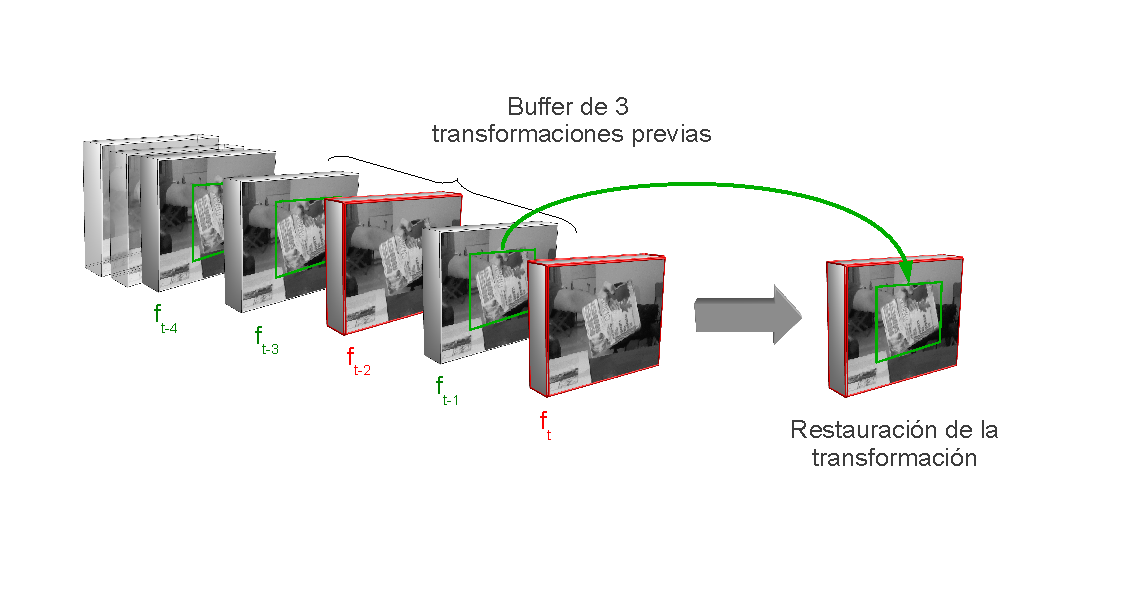
\includegraphics[scale=0.6]{../../figs/restauracion_transfromacion}
       \caption[\small{Esquema de restauración de la última transformación válida}]{\small{Esquema de restauración de la última transformación válida.}}
    \label{fig:restauracion_transformacion} 
  \end{figure}
\end{frame}
\subsection*{}
\begin{frame}{RA en el flujo de video}
  \begin{itemize}
    \item Se utiliza $H^{-1}$ para superponer la imagen virtual en la perspectiva correcta en el flujo de video.
      \note[item]{plane (usually the imager plane) by the following simple eqns: 
      p_dest = H * p_src,  p_src = H^ -1 * p_dest 
      In this case, p_dest is the image plane, p_src is the world plane. To solve for the world pts, use the 2nd equn above}
      \note[item]{H mapea puntos de una primer imagen a puntos en una segunda imagen}
    \item Existe una interpolación debido a la transformación de píxeles.
  \end{itemize}

  \begin{figure}[tbhp]
   \centering
        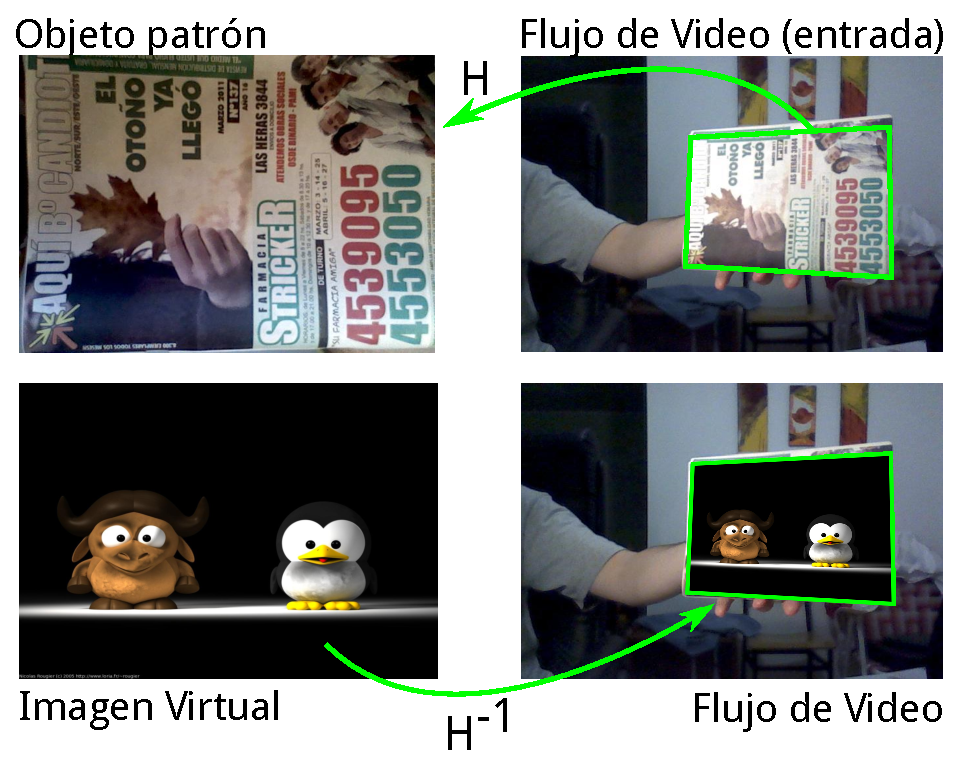
\includegraphics[scale=0.4]{../../figs/transfperspectiva_presentacion}
    \caption[\small{Esquema de transformación perspectiva}]{\small{Esquema de transformación perspectiva utilizando la homografía $H$.}}
   \label{fig:transf_pespectiva}
  \end{figure}
\end{frame}
     \section{Experimentos y Resultados}
\subsection{Entorno de pruebas e imágenes} %(prototipos) para realizar las pruebas
    \begin{frame}{Definición de imágenes}
      \begin{itemize}
	\item<1-> \textbf{Imagen patrón}: detectar y seguir en cada fotograma del flujo de video. En su lugar se superpone el objeto de realidad aumentada.
	Restricciones prácticas:
	  \begin{enumerate}
	  \item \small tamaño de $640 \times 480$ píxeles,
	  \item \small condiciones de iluminación adecuadas,
	  \item \small imagen debe ser rica en detalles,
	  \item \small plano de la imagen perpendicular al lente de la cámara al momento de la captura.
	  \end{enumerate}

	\item<2-> \textbf{Imagen objetivo}: es un fotograma del flujo de video, adquirido con la cámara web en tiempo real.
	
	\item<3-> \textbf{Objeto de realidad aumentada}: imagen, video, texto, etc. \note[item]{no visual: sonido, plano de un objeto 3d}
      \end{itemize}
    \end{frame}
    
    \begin{frame}{Herramientas}
      \begin{block}{Software}
	\begin{itemize}
	 \item OpenCV 2.3.1.
	 \item C$\slash$C++.
	\end{itemize}
      \end{block}
      \begin{block}{Hardware}
	\begin{itemize}
	  \item Webcam: Resolución de $640 \times 480$ píxeles.
	  \item Procesador Intel® Core 2 Duo 2.2 Ghz., 4Gb. RAM.
	\end{itemize}
      \end{block}
    \end{frame}

    \begin{frame}{Imagen patrón y condiciones de iluminación}
      \begin{itemize}
	\item Imagen patrón: tapa de una revista de $22 \times 17$ cm.
	\item Tres condiciones de iluminación diferentes:
	\begin{enumerate}
	  \item<1-> \textbf{Iluminación normal $(B_{N})$}: 
		\begin{itemize}
		  \item lámpara de bajo consumo de 18 W (90 W. de una lámpara incandescente).
		\end{itemize}
    
	  \item<2-> \textbf{Iluminación alta $(B_{H})$}: 
		  \begin{itemize}
		  \item $(B_{N})$ + iluminación direccional con lámpara incandescente de 60 W.
		  \end{itemize}
	      
	  \item<3-> \textbf{Iluminación baja $(B_{L})$}:
		  \begin{itemize}
		    \item Dificultad para la lectura de un documento.
		    \item Lámparas apagadas.
		  \end{itemize}  
	\end{enumerate}
      \end{itemize}
    \end{frame}
  
  \begin{frame}{Entorno ambiental}
      \begin{figure}[tbhp]
	\centering
	      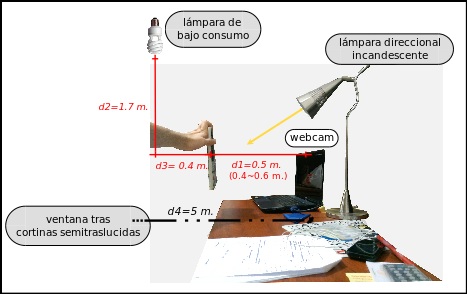
\includegraphics[scale=0.45]{../../figs/entorno/entorno_pruebas_slide}
	  \caption*{Esquema del ambiente en el que se realizaron las pruebas.}
	\label{fig:entorno_pruebas}
      \end{figure}
  \end{frame}
    
\subsection{Experimentos}%Pruebas realizadas
\begin{frame}{Experimentos}
  \begin{block}{Experimento 1: costo computacional y detección de puntos}
  Evaluación del costo computacional y detección de puntos claves bajo las condiciones de iluminación $B_{N}$, $B_{H}$ y $B_{L}$.
  \end{block}
\end{frame}
%%%%%%%%%%%%%%%%%%%%%%%%%%%%%%%%%%%%%%%%%%%%%%%%%%%%%%%%%%%%%%%%%%%%%%%%%%%%%%%%%%%%%%%%%%%%%%%%%%%
\subsubsection*{Experimento 1}
  \label{subsec:paraqumetros_utilizados}
  
  \begin{frame}{Experimento 1}
   \begin{itemize}
  \item Se capturó la imagen patrón en las tres condiciones de iluminación.
      \begin{figure}[H]
      \centering
      \subfloat[\scriptsize{Imagen patrón con condición $B_{N}$.}]{
\includegraphics[width=0.32\textwidth]{../../exp1/train_normal_BN/train_normal} \label{fig:train_normal}}
      \subfloat[\scriptsize{Imagen patrón con condición $B_{H}$.}]{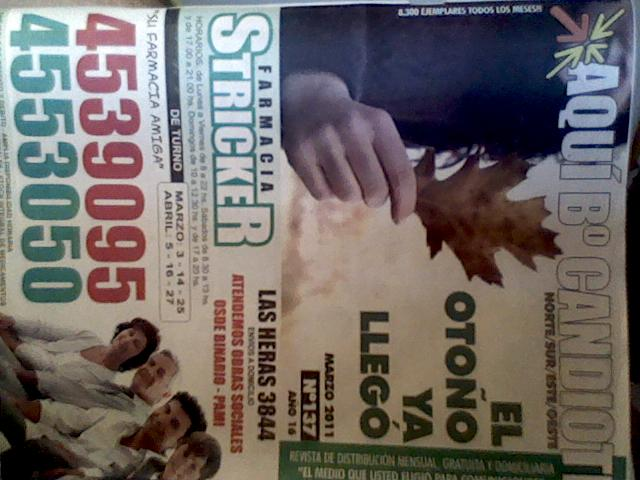
\includegraphics[width=0.32\textwidth]{../../exp1/train_brillante_BH/train_brillante} \label{fig:train_brillante}}
      \subfloat[\scriptsize{Imagen patrón con condición $B_{L}$.}]{
\includegraphics[width=0.32\textwidth]{../../exp1/train_oscura_BL/train_oscura} \label{fig:train_oscura}}
      \caption*{Imágenes obtenidas para condiciones de iluminación diferentes.}
      \label{fig:prueba_iluminacion_realce_detalles_2_imagenes}
    \end{figure}
  \item Se aplicó a cada una de las imágenes operaciones para realce de detalles y mejora en la iluminación.
 \end{itemize}
  \end{frame}
  
  

% \begin{frame}{Condición $B_{N}$}
% \note[item]{\textit{filtrado pasa altos}, \textit{filtro de alta potencia} $\rightarrow$ realza los detalles}
% \note[item]{\textit{ecualización} $\rightarrow$ mejora el contraste}
%   \begin{figure}
%     \centering
%     \subfloat[\tiny{Imagen patrón con Ilum. $B_{N}$}]{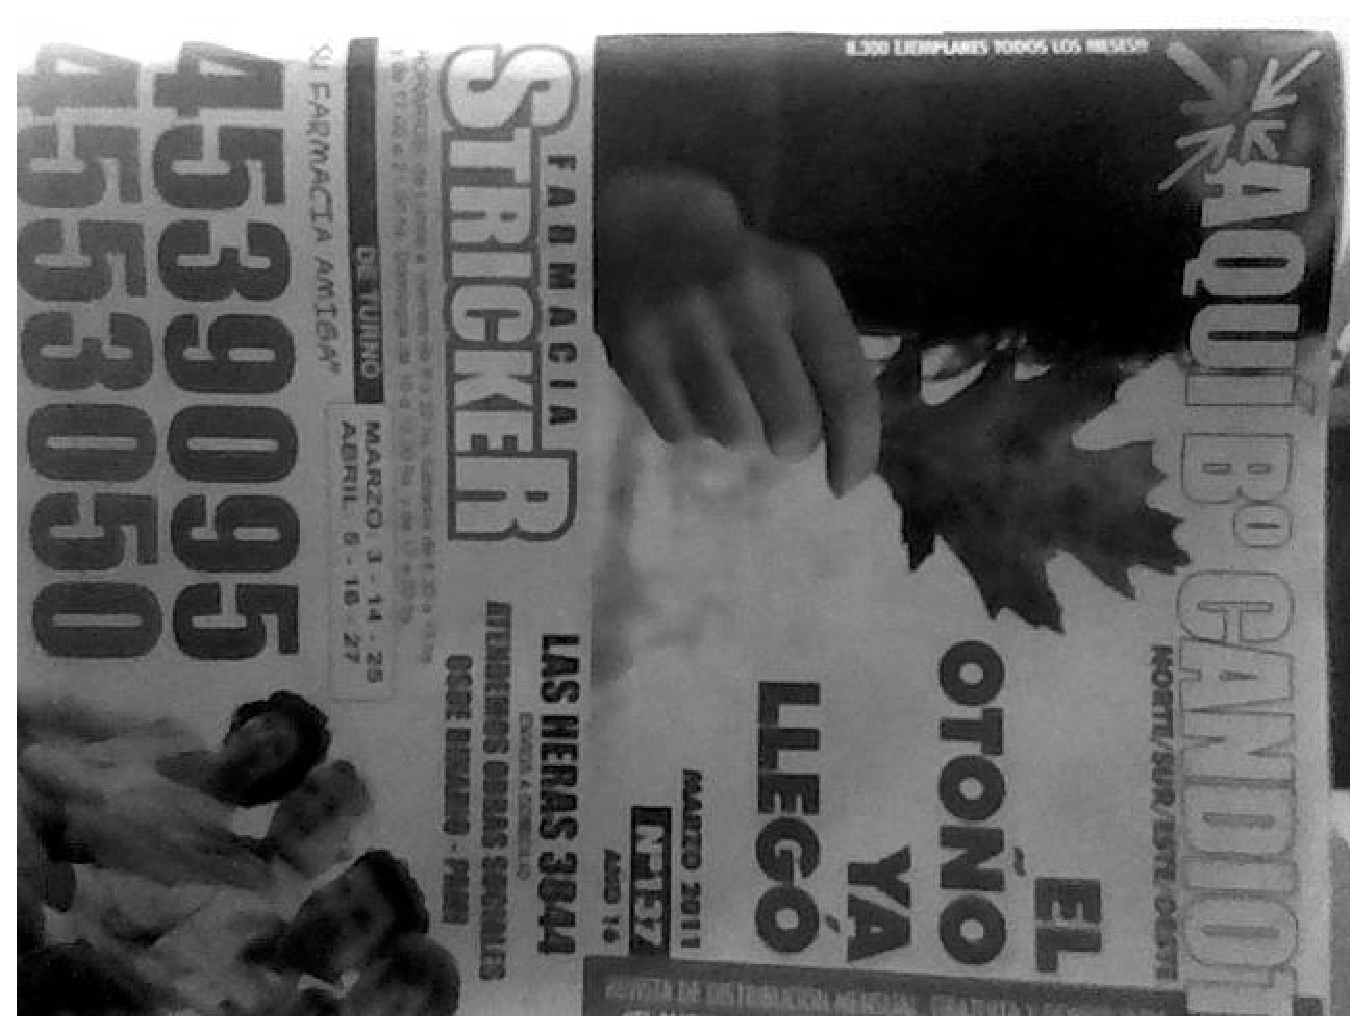
\includegraphics[width=0.32\textwidth]{../../exp1/train_normal_BN/train_normal_grises} \label{fig:iluminacion_BN_original}}
%     \subfloat[\tiny{Transformación logarítmica}]{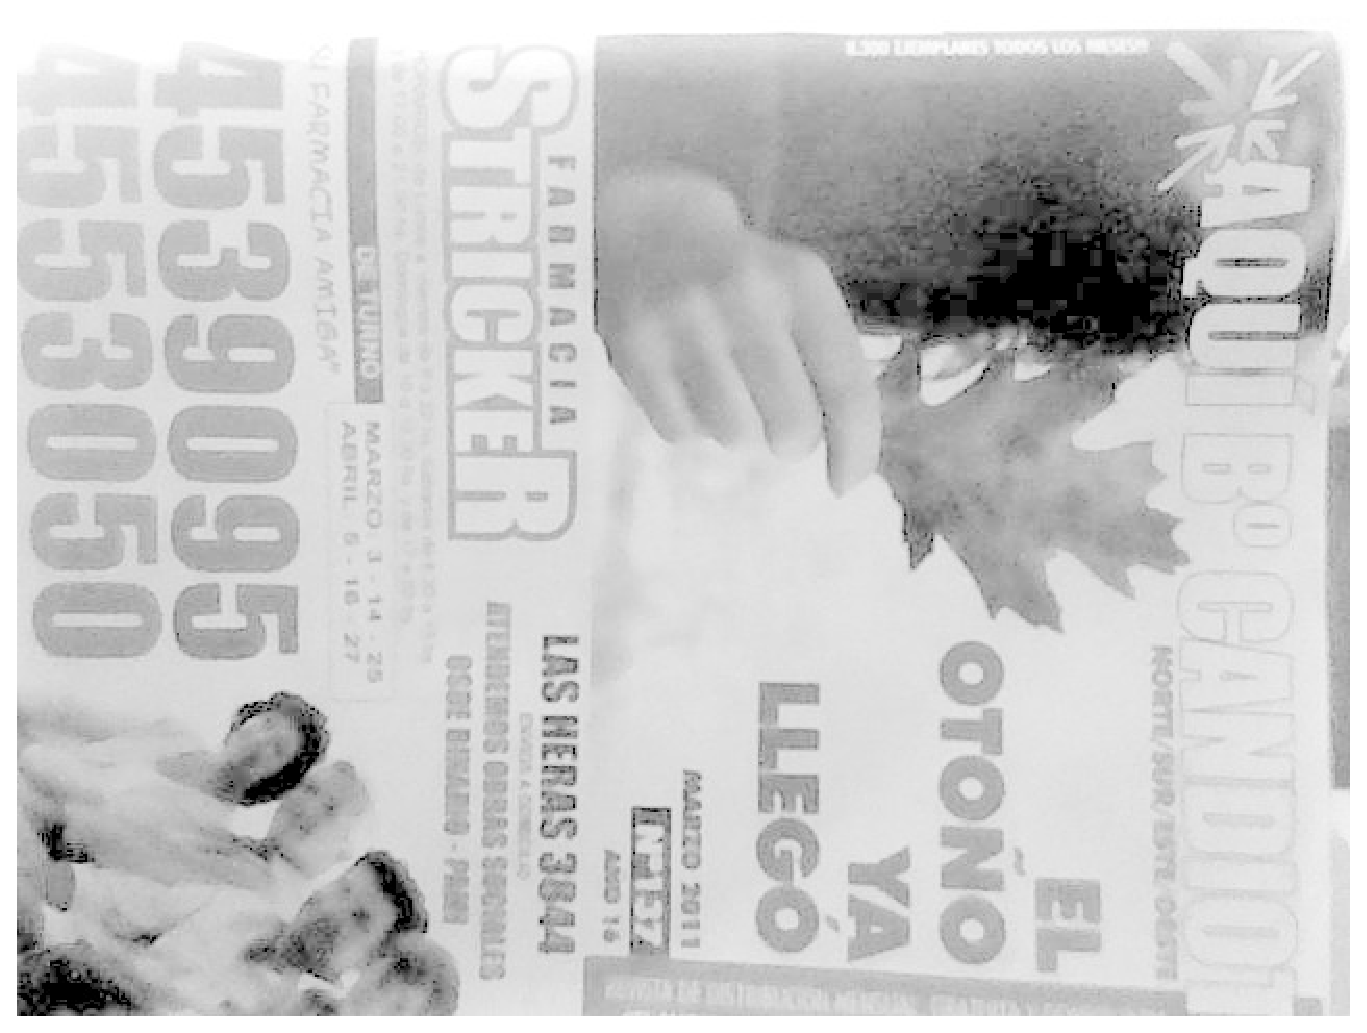
\includegraphics[width=0.32\textwidth]{../../exp1/train_normal_BN/train_normal_515} \label{fig:iluminacion_BN_logaritmica}}
%     \subfloat[\tiny{Ecualización}]{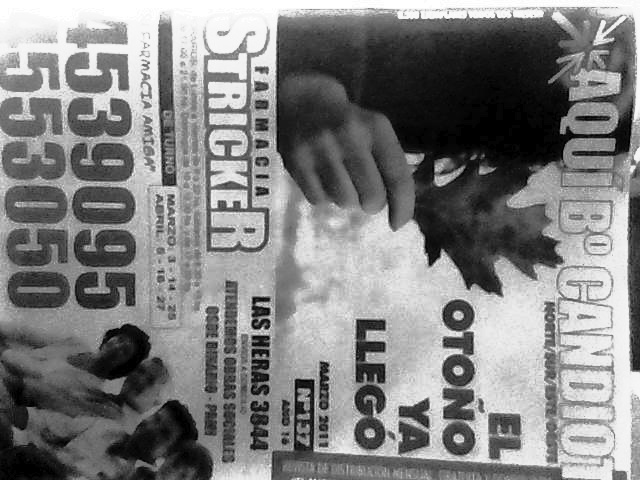
\includegraphics[width=0.32\textwidth]{../../exp1/train_normal_BN/keypoints2} \label{fig:iluminacion_BN_ecualizacion}}\\
%     \subfloat[\tiny{Filtrado pasa altos}]{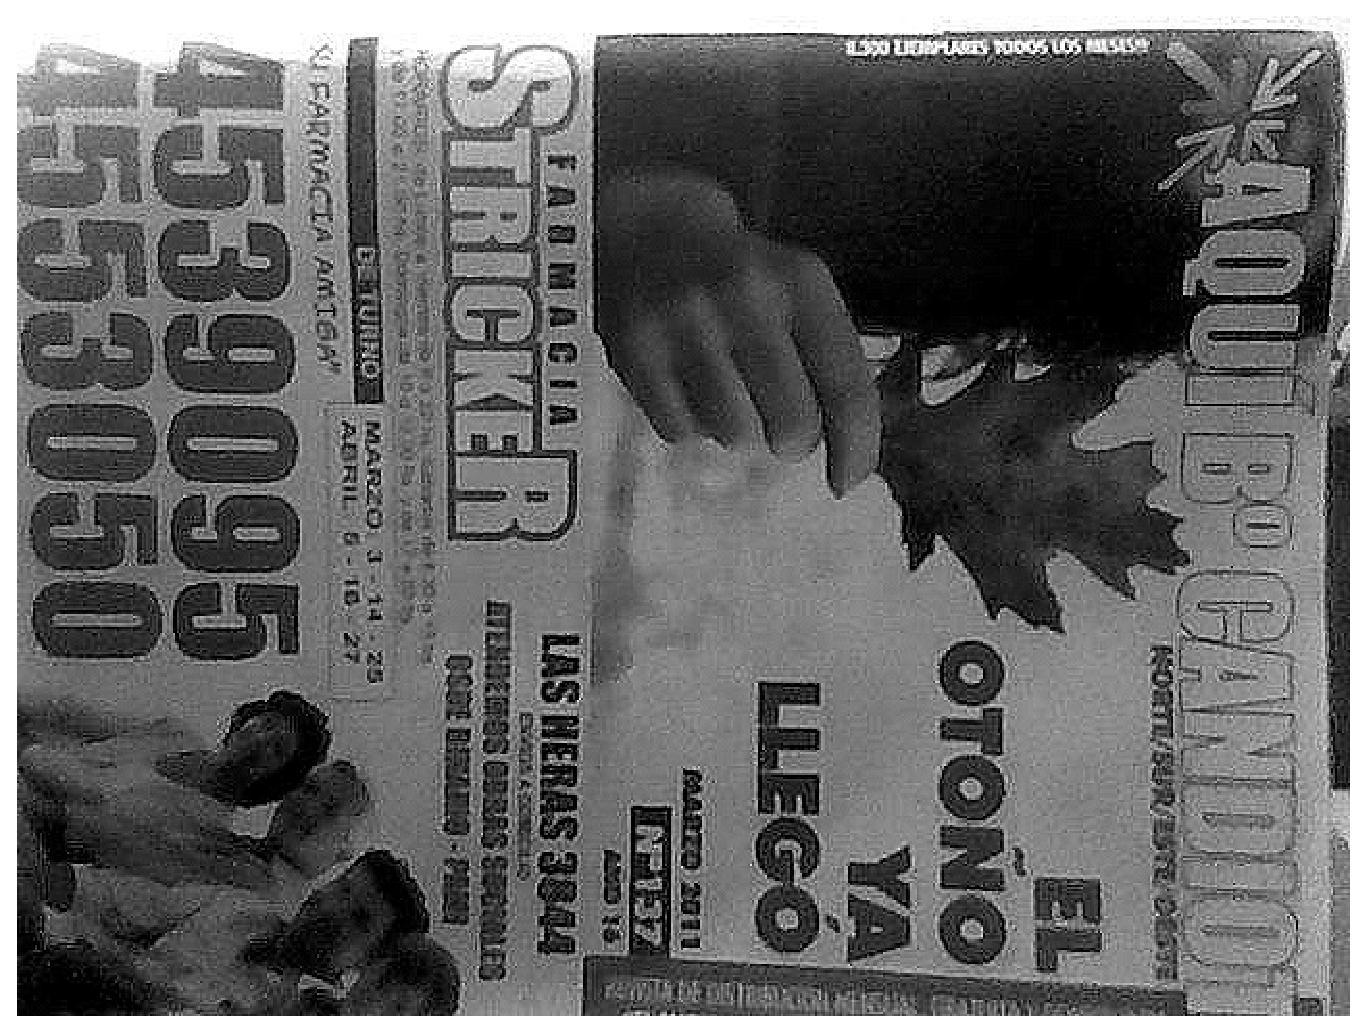
\includegraphics[width=0.32\textwidth]{../../exp1/train_normal_BN/keypoints3} \label{fig:iluminacion_BN_pasaaltos}}
%     \subfloat[\tiny{Filtrado de alta potencia}]{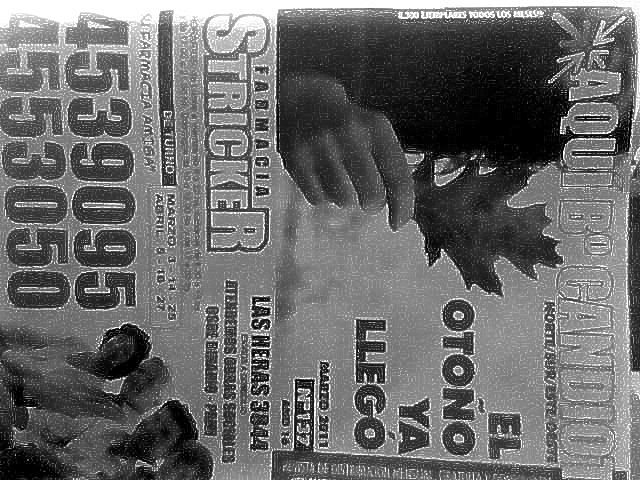
\includegraphics[width=0.32\textwidth]{../../exp1/train_normal_BN/keypoints4} \label{fig:iluminacion_BN_altapotencia}}
%     \subfloat[\tiny{Ecualización + filtrado de alta potencia}]{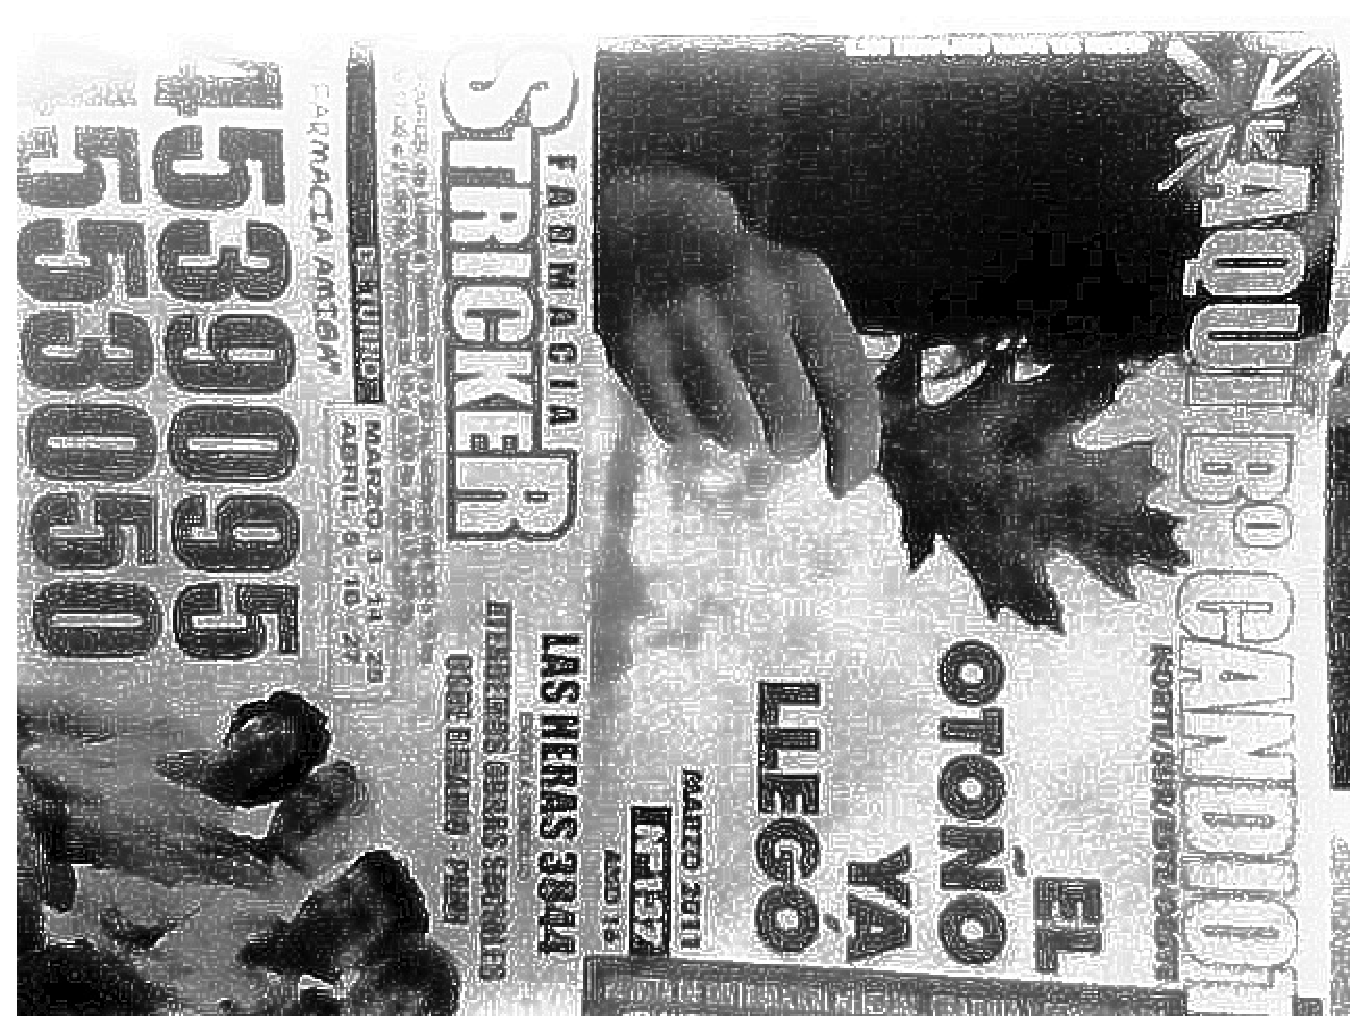
\includegraphics[width=0.32\textwidth]{../../exp1/train_normal_BN/keypoints5} \label{fig:iluminacion_BN_ecyaltapotencia}}\\
% %     \caption*[Resultados de aplicar las técnicas para la mejora en iluminación y detalles en condición $B_{N}$]{Resultados de aplicar las técnicas para la mejora en iluminación y detalles en condición $B_{N}$.}
%     \label{fig:mejoras_iluminacion_normal_BN}               %% Etiqueta para la figura entera
%   \end{figure}
% \end{frame}

% \begin{frame}{Condición $B_{H}$}
%     \begin{figure}
%       \centering
%       \subfloat[\tiny{Imagen patrón con Ilum. $B_{H}$}]{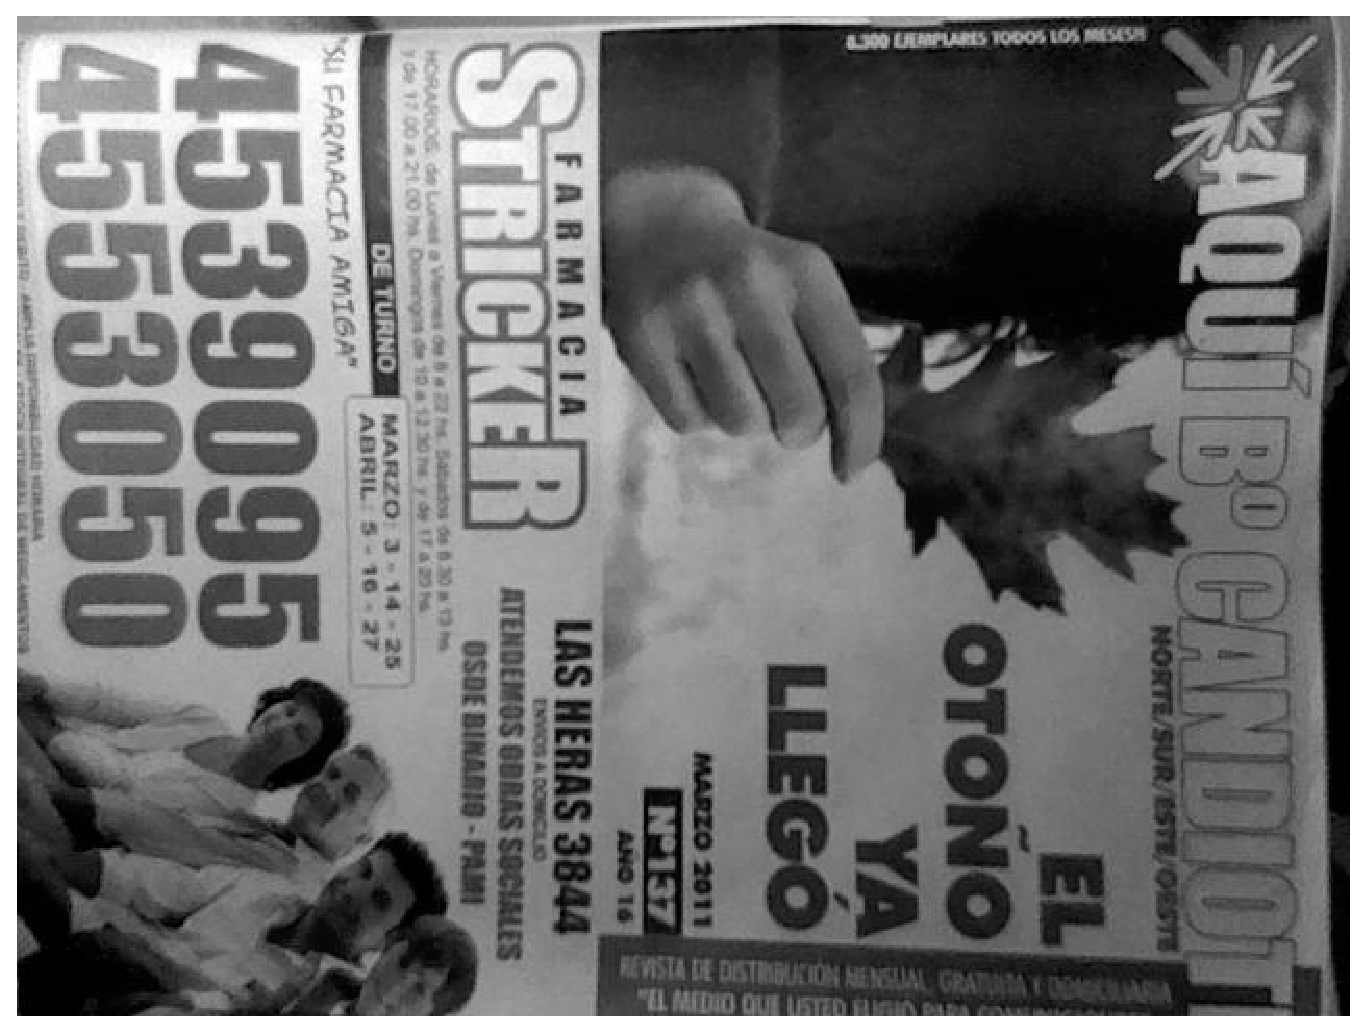
\includegraphics[width=0.32\textwidth]{../../exp1/train_brillante_BH/train_brillante_grises} \label{fig:iluminacion_BH_original}}
%       \subfloat[\tiny{Transformación logarítmica}]{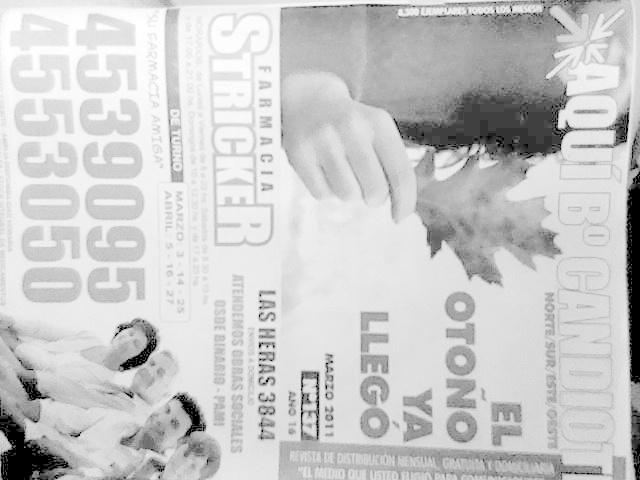
\includegraphics[width=0.32\textwidth]{../../exp1/train_brillante_BH/train_brillante622} \label{fig:iluminacion_BH_logaritmica}}
%       \subfloat[\tiny{Ecualización}]{\includegraphics[width=0.32\textwidth]{../../exp1/train_brillante_BH/keypoints2} \label{fig:iluminacion_BH_ecualizacion}}\\
%       \subfloat[\tiny{Filtrado pasa altos}]{\includegraphics[width=0.32\textwidth]{../../exp1/train_brillante_BH/keypoints3} \label{fig:iluminacion_BH_pasaaltos}}
%       \subfloat[\tiny{Filtrado de alta potencia}]{\includegraphics[width=0.32\textwidth]{../../exp1/train_brillante_BH/keypoints4} \label{fig:iluminacion_BH_altapotencia}}
%       \subfloat[\tiny{Ecualización + filtrado de alta potencia}]{\includegraphics[width=0.32\textwidth]{../../exp1/train_brillante_BH/keypoints5} \label{fig:iluminacion_BH_ecyaltapotencia}}
% %       \caption*[Resultados de aplicar las técnicas para la mejora en iluminación y detalles en condición $B_{H}$]{Resultados de aplicar las técnicas para la mejora en iluminación y detalles en condición $B_{H}$}
%       \label{fig:mejoras_iluminacion_brillante_BH}               %% Etiqueta para la figura entera
%     \end{figure}
% \end{frame}

%%%%%%%%%%%%%%%%%%%%%%%%%%%%%%%%%%%%%%%%%%%%%%%%%%%%%%%%%%%%%%%%%%%%%%%%%%%%%%%%%%%%%%%%%%%%%%%%%%%
\begin{frame}{Condición $B_{L}$}
\note[item]{Mejores resultados para $B_{L}$ $\rightarrow$ \textit{ecualización}: Maximización del contraste y combinación de \textit{ecualización y filtrado de alta potencia}}
  \begin{figure}
  \centering
  \subfloat[\scriptsize{Imagen patrón con Ilum. $B_{L}$}]{\includegraphics[width=0.32\textwidth]{../../exp1/train_oscura_BL/train_oscura_grises} \label{fig:iluminacion_BL_original}}
  \subfloat[\scriptsize{Transformación logarítmica}]{\includegraphics[width=0.32\textwidth]{../../exp1/train_oscura_BL/train_oscura453} \label{fig:iluminacion_BL_logaritmica}}
  \subfloat[\scriptsize{Ecualización}]{\includegraphics[width=0.32\textwidth]{../../exp1/train_oscura_BL/keypoints2} \label{fig:iluminacion_BL_ecualizacion}}\\
  \subfloat[\scriptsize{Filtrado pasa altos}]{\includegraphics[width=0.32\textwidth]{../../exp1/train_oscura_BL/keypoints3} \label{fig:iluminacion_BL_pasaaltos}}
  \subfloat[\scriptsize{Filtrado de alta potencia}]{\includegraphics[width=0.32\textwidth]{../../exp1/train_oscura_BL/keypoints4} \label{fig:iluminacion_BL_altapotencia}}
  \subfloat[\scriptsize{Ecualización + filtrado de alta potencia}]{\includegraphics[width=0.32\textwidth]{../../exp1/train_oscura_BL/keypoints5} \label{fig:iluminacion_BL_ecyaltapotencia}}
%   \caption*[Resultados de aplicar las técnicas para la mejora en iluminación y detalles en condición $B_{L}$]{Resultados de aplicar las técnicas para la mejora en iluminación y detalles en condición $B_{L}$}
  \label{fig:mejoras_iluminacion_oscura_BL}               %% Etiqueta para la figura entera
  \end{figure}
\end{frame}

\begin{frame}{Tiempos y cantidad de características}
    Umbral hessiano: $700$ e igual para las tres condiciones de iluminación. 
	\note[item]{el umbral se estableció empíricamente}
    \begin{table}[htbp]
      \caption*{Tiempo de procesamiento en milisegundos y cantidad de características sobre la imagen patrón en condiciones de iluminación $B_{N}$, $B_{H}$ y $B_{L}$.}
	\begin{tabular}{|l|r|c|c|c|}
	  \hline
	  %& \multicolumn{2}{c|}{\textbf{Iluminación Normal}} \\ \hline
	  & \multicolumn{1}{c|}{\textbf{t [ms]}} & \textbf{$B_{N}$} & \textbf{$B_{H}$} & \textbf{$B_{L}$}\\ \hline
	  \textbf{Sin Proc} & 0,00 &  958 & 1297 & 154\\ \hline
	  \textbf{Logaritmo} & 7,15 & 702 & 950 & 83\\ \hline \note[item]{Tiempo del logaritmo superior, se cree que es por la forma en que fue implementado (openCV trae implementado el log neperiano  y no el en base 10. La compilación de la librería con Intel IPP podría mejorar. Como la cantidad de puntos característicos es menor (excepto cuando hay baja iluminación), no se le dio importancia.)}
	  \textbf{Ecualización} & \textbf{0,70} & 1546 & 1472 & 1233\\ \hline
	  \textbf{F. Pasa Altos} & 1,26 &  1633 & 2006 & 269\\ \hline
	  \textbf{F. Alta Pot.} & 3,10 & 1952 & 2216 & 353\\ \hline \note[item]{F. Pasa altos y alta potencia: Las técnicas que involucran una operación de convolución obtienen tiempos mayores que las demás}
	  \textbf{Ec.+F. Alta Pot.} & 4,31 & \textbf{2704} & \textbf{2443} & \textbf{2002}\\ \hline 
	\end{tabular}
	\note[item]{combinación de ec. y F. de alta potencia resulta mayor por ser la suma de las dos anteriores}
	\note[item]{Tiempos: $\textrm{Sin proc.}<\textrm{Ec.}<\textrm{F. P. Altos}<\textrm{F. Alta pot.}<\textrm{Ec.+F. Alta Pot}<\textrm{log}$}
      \label{tabla:tiempos_realce_iluminacion}
    \end{table}    
\end{frame}

\begin{frame}{Cantidad de características}
% En el gráfico de la Fig. \ref{graph:comparacion_cantptos} se presenta una comparación de la cantidad de puntos detectados para las condiciones $B_{N}$, $B_{H}$ y$B_{L}$ establecidas. Claramente se advierte que cuando se realiza la combinación de \textit{ecualización y filtrado de alta potencia} en el caso de un ambiente en condición $B_{N}$, la cantidad de puntos detectados casi llega a triplicarse, respecto de cuando no se aplica técnica alguna. En tanto que en una condición $B_{H}$, la detección se duplica. Si analizamos lo que pasa en la condición de iluminación $B_{L}$, la cantidad de características posee valores bajos respecto de las otras condiciones de iluminación, ésta diferencia se evidencia aún más cuando no se aplica la ecualización, ya que los \textit{filtros pasa altos y de alta potencia} actúan sobre una imagen oscura sobre la que realzan los detalles, pero la diferencia de grises entre píxeles vecinos resulta insuficiente para una correcta detección.
  \note[item]{Marcelo: Explicar bien el gráfico que es lo que se ve y observa. Cuanto más largas las barras mejor es. En todos los casos se mejora y queda a criterio del usuario usar una u otra. NO EXPLICAR EL LOGARITMO}
  \note[item]{Marcelo: no se entendió la gráfica de tiempos, nombrarla mejor!}
  \begin{figure}[tbhp]
   \centering
        \includegraphics[scale=0.38]{../../pruebas_modif/graph_ptos_realces_presentacion1}
%     \caption*{\tiny{Cantidad de puntos detectados para la imagen con luminosidad normal (Fig. \ref{fig:train_normal}), alta (Fig. \ref{fig:train_brillante}) y baja (Fig. \ref{fig:train_oscura}).}}
   \label{graph:comparacion_cantptos}
  \end{figure}
   \note[item]{En $B_{N}$, la Ec.+filtrado de Alta Pot. la cant. de puntos se triplica. En $B_{H}$ se duplica respecto de Sin Proc.}
   \note[item]{Cant. de caract. detectadas $B_{N}$ y $B_{H}$: $\textrm{Log.}<\textrm{Sin proc.}<\textrm{Ec.}<\textrm{F.P altos}<\textrm{F.A.potencia}<\textrm{Ec.+F.A.potencia}$}
   \note[item]{Cant. de caract. detectadas $B_{L}$: $\textrm{Sin proc.}<\textrm{F.P altos}<\textrm{F.A.potencia}<\textrm{Log.}<\textrm{Ec.}<\textrm{Ec.+F.A.potencia}$}
   \note[item]{Combinacion de ec y filtro de alta pot, es la que mayor cantidad de detecciones de puntos presenta, producto de una iluminación más uniforme y luego el realce de los detalles.}
   \note[item]{Pasa altos y alta potencia realzan las altas frecuencias y discontinuidades. Alta potencia detecta más que el pasa altos porque no afecta las bajas frecuencias.}
   \note[item]{ecualización se obtienen más puntos que sin procesamiento, puede considerarse útil si la prioridad es el tiempo}
   \note[item]{Log solo incrementa puntos en la imagen con condición de iluminación baja. En condiciones de iluminación normal y alta el Log detecta menos características porque poseen intensidades más homogéneas y por lo tanto menor distinción en los detalles. En baja iluminación se incrementa como consecuencia de la expansión del rango dinámico}
\end{frame}

\begin{frame}{Experimento 1: conclusiones}
  \begin{itemize}
   \item En condiciones $B_{N}$ y $B_{H}$ resultados aceptables sin pre-procesamiento de iluminación o realce de detalles.
      \note[item]{Aplicar las técnicas que aumentan la cantidad de características, mejora la cantidad de características pero repercuten en el tiempo de procesamiento}
   \item Aplicar técnicas repercute negativamente en el tiempo de procesamiento pero aumenta la cantidad de puntos detectados.
   \item Determinar técnicas a utilizar y umbral hessiano:
      \begin{itemize}
	\item ¿Qué se desea priorizar: calidad en la detección o velocidad de ejecución?
	\item ¿Cuáles son las condiciones del ambiente? \note[item]{condiciones de iluminación}
      \end{itemize}
   \end{itemize}
\end{frame}

\begin{frame}{Experimento 1: conclusiones}
Prueba en condición de iluminación baja ($B_{L}$).
 \begin{itemize}
    \item En la práctica se presentan casos de detección ``intermitente'' o nula en condición $B_{L}$.
%       \begin{itemize}
% 	\item 
% 	\item condiciones intermedia entre $B_{L}$ y $B_{N}$
%       \end{itemize}
      \note[item]{Obtener mayor cantidad de características no presenta garantías de lograr una mejor detección (existencia de posibles características espurias)(*). SIN EMBARGO!}
  \end{itemize}
   
  \begin{itemize}
    \item La ecualización o ecualización+filtro de alta potencia mejoran la detección.
    \item Aumentar la cantidad de características produce una mejora en la detección. 
	\note[item]{Aumentar en el sentido de aplicar un realce de iluminación y no  de variar el umbral hessiano.}
    \item Una variación del umbral no produce resultados significativamente mejores. 
	\note[item]{No alcanza a detectar las características por ser muy oscura la imagen. Esto no tiene que ver con el umbral hessiano.}
  \end{itemize}
\end{frame}

\subsubsection*{}
\begin{frame}{Experimento 2}
\note[item]{Marcelo: no decir estables! sino que se quería obtener conclusiones en los ambientes donde el método es probable que sea ejecutado en condiciones de iluminación normal y alta}
\begin{block}{Experimento 2: costo computacional del método propuesto}
 Evaluación detallada del costo computacional en etapa de ejecución, considerando los pasos del algoritmo propuesto.
\end{block}
 \begin{itemize}
  \item Tiempos que insumen los procesos del método.
  \note[item]{Condicionales del método que permiten mejorar la detección y minimizar los tiempos de procesamiento}
  \item 2 pruebas en condiciones de iluminación $B_{N}$ y $B_{H}$. \note[item]{no se usa $B_{L}$ por efecto de ``parapadeo'' y se desean obtener conclusiones cuando la detección resulta estable}
  \item Sin técnicas de ``Pre-Procesamiento de iluminación y realce de detalles''. \note[item]{se dejan a criterio del usuario y para las condiciones de iluminación dadas no fue necesario aplicarlas}
  \note[item]{Marcelo: Decir bien ``Pre procesamiento de iluminación y realce de detalles''}
 \end{itemize}
\end{frame}
 
 \begin{frame}{Pruebas}
 \note[item]{Marcelo: Se hicieron pruebas para 2 videos sobre el flujo de video}
 \note[item]{Se realizaron 2 pruebas}
      \begin{block}{Prueba 1 (P1)}
	  \begin{itemize}
	    \item Duración: 1:50 minutos.
	    \item Umbral hessiano: 3500.
	    \item Imagen con condición $B_{N}$.% \ref{fig:train_normal} \footnote{Video de la prueba: \url{http://youtu.be/E8uGptzdEiw}}
	  \end{itemize}
      \end{block}

      \begin{block}{Prueba 2 (P2)}
	  \begin{itemize}
	    \item Duración: 1:35 minutos.
	    \item Umbral hessiano: 5000.
	    \item Imagen con condición $B_{H}.$% \ref{fig:train_brillante} \footnote{Video de la prueba: \url{http://youtu.be/Pkiub9ZXP4k}}
	  \end{itemize}
	  \note[item]{por cuestiones de brevedad se presenta la p1 solamente ya que con esta se obtuvieron resultados similares}
      \end{block}
\end{frame}

% \begin{frame}{Datos computados}
%   \begin{itemize}\small{
%     \item Tiempo de \textit{detección de movimiento},
%     \item Tiempo de \textit{extracción y descripción de las características en BR} *,
%     \item Tiempo de \textit{búsqueda de correspondencias} *,
%     \item Tiempo de \textit{estimación de la homografía} *,
%     \item Tiempo de comprobación \textit{contorno convexo y vértices válidos} *,
%     \item Tiempo de \textit{transformación perspectiva de la imagen de RA utilizando la homografía} *,
%     \item Cuadros por segundo (FPS),
%     \item Total de puntos detectados en la imagen patrón,
%     \item Total de puntos detectados en la imagen objeto,
%     \item Total de coincidencias potencialmente válidas.
%   }
%   \end{itemize}
% \end{frame}

% \begin{frame}{Análisis de 2 procesos}
%     \begin{block}{``Proceso con bifuración en condicionales (\textbf{PCBC})''}
% 	Las operaciones marcadas con (*) pueden ignorarse en el ciclo de ejecución sin impedir que se realice el enriquecimiento de la realidad.
% 	  \note[item]{Las operaciones marcadas con (*) pueden ignorarse.}
% 	  \note[item]{SI la comprobación de contornos convexos y vértices válidos (CCVV) no se cumple, entonces no se calcula la Transformación Perspectiva(TP)}
% 	  \note[item]{si la homografía no es detectada, no se realiza la CCCV y por ende tampoco la TP}
% 	  \note[item]{si no se detecta movimeinto en la escena, ninguno de los procesos es ejecutado}
% 	  \note[item]{Todos estos condicionales produce que el tiempo rpomedio de procesamiento disminuya cuando alguna o todas las operaciones son ignoradas}
%     \end{block}
%     \begin{block}{``Proceso sin bifuración en condicionales (\textbf{PSBC})''}
%     \end{block}
% \end{frame}

\begin{frame}{Tiempos de operación de procesos en P1}
  \note[item]{Marcelo: Aclarar que cuanto menor son las barras mejor es el método}
  \note[item]{Marcelo: Aclarar que existe un método estándar en donde los condicionales no están y el método propuesto por nosotros.}
  \begin{figure}[tbhp]
   \centering
        \includegraphics[scale=0.38]{../../pruebas_modif/3500_sinproc/graph_tiempos_3500_presentacion1}
    \caption*{\tiny{Tiempos promedios de operación por procesos en la prueba 1}}
   \label{graph:graph_tiempos_3500}
  \end{figure}
  \note[item]{+comprobación de área BR, y luego actuación del buffer (condición de presencia previa => mejoran aún más)}
  \note[item]{Tiempos promedios en la fase de ejecución de P1 para el método estándar y el propuesto.}
  \note[item]{Proceso de extracción y descripción de características es el que más tiempo consume a pesar de realizarse en BR: \begin{itemize}
	\item Si BR = 50\% de la imagen patrón de $640 \times 480$ píxeles $\rightarrow$ representa un 42\% del tiempo para procesar toda la imagen
      \end{itemize}
  }
  \note[item]{Segundo aparece la estimación de la homografía por tratarse de un método iterativo que estima la matriz H y refina las coincidencias}
  \note[item]{Tercero queda la transofmración perspectiva que involucra una interpolación}
  \note[item]{Sigue la búsqueda de correspondencias (recordar que es aproximada y se utilizó randomized kdtrees)}
  \note[item]{sigue la detección de movimiento y la CCVV que están compuestas de operaciones triviales}
\end{frame}
% 
% \begin{frame}{P1}
% 
% \end{frame}

\begin{frame}{Conclusiones P1}
% tiempos en los diferentes procesos
%  \begin{itemize}
%   \item extracción y descripción de características es la que más tiempo requiere (a pesar de que se minimizó el procesamiento en un área de la imagen (BR)). Si el área BR en el que se extraen características es del 50\% de la imagen patrón en $B_{N}$} el tiempo de procesamiento representa un 42\% del tiempo total que se requería para extraer las características en la totalidad de la imagen.
%   \item segundo proceso que más tiempo consume es la estimación de la homografía por tratarse de un método iterativo que estima la matriz $H$ y refina las coincidencias
%   \item transformación perspectiva en tercer lugar por involucrar una interpolación,
%   \item les siguen búsqueda de correspondencias, la detección de movimiento y finalmente, la CCVV que está compuesta de operaciones triviales
%  \end{itemize}

%  total de puntos detectados y las potenciales correspondencias válidas
  \begin{block}{Objetivas}
      Tiempos:
      \begin{itemize}
	  \item Método estándar: $6.93$ FPS promedio.
	  \item Método propuesto: $28.35$ FPS promedio.
      \end{itemize}
  \end{block}
  
  \begin{block}{Subjetivas}
      \begin{itemize}
	  \item Eliminación de transformaciones fallidas.
	  \item Reducción de detecciones intermitentes.
	    \note[item]{Marcelo: El objeto virtual se sigue dibujando si se pierde en un frame. si pasa más de 3 frames perdidos, se deja de dibujar}
	    \note[item]{Marcelo: Ver si no me falta alguna conclusión más?}
	  \item Mayor fluidez en la reproducción. \note[item]{Naturalidad}
      \end{itemize}
  \end{block}
 %   \item segundo proceso que más tiempo consume es la estimación de la homografía por tratarse de un método iterativo que estima la matriz $H$ y refina las coincidencias
%   \item transformación perspectiva en tercer lugar por involucrar una interpolación,
%   \item les siguen búsqueda de correspondencias, la detección de movimiento y finalmente, la CCVV que está compuesta de operaciones triviales
%  
%  \begin{exampleblock}{Puntos y coincidencias}
%     \begin{itemize}
% 	\item 192 puntos claves en la imagen patrón
% 	\item en promedio 130 puntos en la imagen del flujo de video
% 	\item en promedio 38 pares de coincidencias potencialmente válidas (máximo de 81 pares)
%     \end{itemize}
%  \end{exampleblock}
\end{frame}

\begin{frame}{Imágenes prueba 1}
%   Umbral hessiano 3500 y la escena se encuentra en condición $B_{N}$ de iluminación.
    \note[item]{Marcelo: Explicar oclusión: en la quinta imagen se puede ver los dedos que están sobre el objeto a detectar y sin embargo se sigue viendo}
    \note[item]{Marcelo: Si la oclusión es por menos de 3 frames sigue funcionando}
    \begin{figure}[tbhp]
    \centering
    \subfloat{\includegraphics[width=0.34\textwidth]{../../pruebas_modif/capturas/usables/train_normal} \label{fig:imagen_patron_ejemplo}}
    \subfloat{\includegraphics[width=0.34\textwidth]{../../pruebas_modif/capturas/usables/pinguino} \label{fig:imagen_objetoar_ejemplo}}
    \subfloat{\includegraphics[width=0.34\textwidth]{../../pruebas_modif/capturas/usables/captured154} \label{fig:imagen_secuencia1_ejemplo}}\\
    \subfloat{\includegraphics[width=0.34\textwidth]{../../pruebas_modif/capturas/usables/captured135} \label{fig:imagen_secuencia2_ejemplo}}
    \subfloat{\includegraphics[width=0.34\textwidth]{../../pruebas_modif/capturas/usables/captured141} \label{fig:imagen_secuencia3_ejemplo}}
    \subfloat{\includegraphics[width=0.34\textwidth]{../../pruebas_modif/capturas/usables/captured207} \label{fig:imagen_secuencia4_ejemplo}}
    \caption*{\tiny{Imagen patrón, objeto de RA y secuencia de imágenes (no sucesivas) con enriquecimiento de la realidad.}}
    \label{fig:secuencia_ejemplo_BN}               %% Etiqueta para la figura entera
    \end{figure}
\end{frame}

% \begin{frame}{Prueba 2}
%   \begin{itemize}
%     \item En $P2$ resultados similares a $P1$
%     \item La cantidad de puntos detectados en la imagen patrón $\uparrow$ a pesar de $\uparrow$ el umbral hessiano $\rightarrow$
%     La imagen sobre la cual se aplicó poseía mayor luminosidad y, por lo tanto mayores detalles apreciables.
%   \end{itemize}
% \end{frame}
%%%%%%%%%%%%%%%%%%%%%%%%%%%%%%%%%%%%%%%%%%%%%%%%%%%%%%%%%%%%%%%%%%%%%%%%%%%%%%%%%%%%%%%%%%%%%%%%%%%%%%%%%%%%%%%%%%%%%%%%%%%%%%%%%%%%%%%%%%%%%%%%%%%%
\subsection{Implementación de prototipos}
  \begin{frame}{Prototipos}
    \begin{itemize}
      \item Se enriquece la realidad mediante una imagen sobre la tapa de una revista.
	  \note[item]{algunos de estos ejemplos los hemos visto en las imágenes a lo largo de la presentación}
      \item Proveer información inherente a un producto comestible de forma publicitaria: video en condición $B_{N}$.
	\note[item]{se mostrará un video al finalizar la presentacion}%\url{http://youtu.be/j1xPZkglJHs}. 
    \end{itemize}
  \end{frame}

  \begin{frame}{Prototipo publicitario}
    \begin{figure}
	\centering
	\subfloat{\includegraphics[width=0.33\textwidth]{../../imgvitina/vitina}\label{fig:prototipo_img_detect}}
	\subfloat{\includegraphics[width=0.33\textwidth]{../../imgvitina/preciosvirtuales}\label{fig:protitpo_img_ar}}
	\subfloat{\includegraphics[width=0.33\textwidth]{../../imgvitina/captured87,000000}\label{fig:first_detect_protitpo}} \\
	\subfloat{\includegraphics[width=0.33\textwidth]{../../imgvitina/captured94,000000}}
	% \subfloat[][]{\includegraphics[width=2.5in]{../imgvitina/captured97,000000}}
	% \subfloat[][]{\includegraphics[width=2.5in]{../imgvitina/captured120,000000}}
	% \subfloat[][]{\includegraphics[width=2.5in]{../imgvitina/captured140,000000}}\\
	\subfloat{\includegraphics[width=0.33\textwidth]{../../imgvitina/captured146,000000}}
	% \subfloat[][]{\includegraphics[width=2.5in]{../imgvitina/captured151,000000}}
	\subfloat{\includegraphics[width=0.33\textwidth]{../../imgvitina/captured176,000000}\label{fig:last_detect_prototipo}}
	\label{fig:ejemplos_protitipos}
    \end{figure}
    \note[item]{Marcelo: Imagen patrón, objeto de realidad aumentada a sobreimprimir en el flujo de video y diferentes capturas en la etapa de ejecución para el prototipo publicitario.}
    \note[item]{si bien se presentaron estos prototipos se pueden llevar a cabo otro tipo de acciones, reproducción de audio, denotar algo en el flujo de video, escribir instrucciones, etc. las posibilidades son infinitas.}
  \end{frame}
%   %mostrar videos:
%   \begin{frame}{Videos}
% %\movie[externalviewer]{placeholder box}{./img1/videos/preproc.mpeg}
% %\hyperlink{./img1/videos/preproc.mpeg}{\beamerbutton{Go somewhere}}
% \href{run:vlc /home/christian/Documentos/universidad/2011/codigo_e_informes/openCV/anteproyecto/tesis/pruebas_modif/3500_sinproc/out.ogv}{\beamerbutton{Prueba P1}}
% \href{run:vlc /home/christian/Documentos/universidad/2011/codigo_e_informes/openCV/anteproyecto/tesis/pruebas_modif/5000_sinproc/out.ogv}{\beamerbutton{Prueba P2}}
% \href{run:vlc /home/christian/Documentos/universidad/2011/codigo_e_informes/openCV/anteproyecto/tesis/pruebas_modif/vitina2-1.ogv}{\beamerbutton{Prototipo publicitario}}
% %\movie[width=3cm,height=2cm,poster]{}{./img1/videos/preproc.mpeg}
% \end{frame}
     \section{Conclusiones}
\begin{frame}{Conclusiones}
 \begin{itemize}
 \item Afianzamiento de los conocimientos en el área de visión computacional.
 \item Se presentó un método para detectar objetos planos (sin marcadores) en un ambiente controlado, mediante la detección de características sobre imágenes obtenidas con una cámara web de computadora,
 \item Introducción de conceptos de RA, detectores de características relevantes y herramientas para detección y seguimiento de objetos,
 \end{itemize}
\end{frame}
%
\begin{frame}{Conclusiones}
 \begin{itemize}
 \item Técnicas simples para realce de detalles e iluminación, de forma que el usuario pueda considerar la aplicación de alguna de ellas de ser necesario,
 \item Aplicación de estrategias y optimización para una correcta detección, sin afectar al tiempo de procesamiento de forma considerable,
 \item Codificación en C++ y utilización de librería OpenCV que permiten la portabilidad a diferentes sistemas operativos,
 \end{itemize}
\end{frame}
%%%%%%%%%%%%%%%%%%%%%%%%%%%%%%%%%%%%%%%%%%%%%%%%%%%%%%%%%%%%%%%%%%%%%%%%%%%%%%%%%%%%%%%%%%%%%%%%%%%%%%%%%%%%%%%%%%%%%%%%%%%%%%%%%%%%%%%%%
\begin{frame}{Trabajos futuros}
\textbf{Corto Plazo:}
\begin{itemize}
 \item GPU y múltiples hilos de procesamiento aplicado al proceso de extracción y descripción de características.
 \item Utilizar para la búsqueda de correspondencias ``nano flann'' en vez de FLANN: eficiencia en tiempo y consumo de memoria.
 \item Selección automática del umbral hessiano para la discriminación de puntos.
\end{itemize}
\end{frame}
%
\begin{frame}{Trabajos futuros}
\textbf{Mediano Plazo:}
\begin{itemize}
 \item Usar otros detectores en el proceso de extracción y descripción de características: MSER, FAST, etc. Comparación en \url{http://bit.ly/hox3gW}.
 \item Investigar e implementar soluciones para el manejo de la oclusión.
\end{itemize}
\end{frame}
%
\begin{frame}{Trabajos futuros}
\textbf{Largo Plazo:}
\begin{itemize}
 \item Implementar una aplicación con interfaz gráfica orientada a un usuario final. Reconocer diferentes imágenes patrón de una BD y llevar a cabo una acción particular para el enriquecimiento de la realidad.
 \item Implementar el sistema en dispositivos móviles (tablets, celulares, etc.).% utilizando ``procesamiento en la nube (cloud computing)''.
\end{itemize}
\end{frame}
     % \begin{frame}[plain]
%  \frametitle{Agradecimientos}
%  
% \end{frame}

\begin{frame}[plain]
  \frametitle{Muchas gracias!}
\begin{center}
\note[item]{Agradecer}
\vspace{-5mm}
  \begin{beamercolorbox}[center,shadow=true,rounded=true]{title}
    Método para detección y seguimiento\\ de objetos con aplicaciones en Realidad Aumentada
  \end{beamercolorbox}
\vs
\footnotesize \emph{Christian Nicolás Pfarher}\\
\scriptsize{\textit{c.pfarher@gmail.com}}\\
\vs
\includegraphics[scale=1.2]{imagenes/sinc}\\
% \hspace{2mm}\includegraphics[height=5.8mm]{imagenes/fichunl}\includegraphics[height=6.2mm]{imagenes/sinc}\\
\vspace{1mm}
{\rmfamily
{\small Centro de {\textcolor{red}{I}}nvestigaci\'on en} {\normalsize {\textcolor{blue}{\bfseries s}}e\~{n}ales}\\[1mm]
{\normalsize sistemas e {\bfseries in}teligencia {\bfseries c}omputacional} \\
}
\vs
{\scriptsize 
Ingeniería en Informática - Universidad Nacional del Litoral
}
\end{center}
\end{frame}
% \title[Método para detección de objetos]{Método para detección y seguimiento de objetos con aplicaciones en Realidad Aumentada}
% \author[Christian Nicolás Pfarher]{
%   \footnotesize \emph{Christian Nicolás Pfarher}\\
%     Director: \emph{Dr. Albornoz, Enrique Marcelo} \\
%     Co-Director: \emph{Dr. Martínez, Cesar}
%   }
% %
% \institute[sinc($i$)-UNL]{
%   {\rmfamily
%   \textbf{Proyecto Final de Carrera}
%   \\
%   \textbf{Ingeniería en Informática}\\
% %     {\small Centro de {\textcolor{red}{I}}nvestigaci\'on en} {\normalsize {\textcolor{blue}{\bfseries s}}e\~{n}ales}\\[1mm]
% %     {\normalsize sistemas e {\bfseries in}teligencia {\bfseries c}omputacional} \\
%   }
%   \vs
% {\scriptsize 
% \emph{Facultad de Ingeniería y Ciencias Hídricas} \\
% \emph{Universidad Nacional del Litoral}\\
% \vs
% }\hspace{2mm}\includegraphics[height=5.8mm]{imagenes/fichunl}\hs\includegraphics[height=6.2mm]{imagenes/sinc}\\
%   \vspace{1mm}
% }
\end{document}